\documentclass[letterpaper,12pt,oneside,final]{book}
%%
%%  Gabarit de mémoire de maîtrise ou thèse de doctorat.
%%  Template for dissertations and theses @ Polytechnique Montreal.

%%  Normalement, il n'est pas nécessaire de modifier ce document
%%  sauf pour établir le langage (français ou anglais) et pour changer les noms des 
%%  fichiers à inclure.
%%  Usually, this document needs to be modified only to set up the language (French or English) 
%%  and to change the names of the files to include.
%%
%%  Version: 2018-07-31
%%
%%  Accepte les caractères accentués dans le document (UTF-8).


\makeatletter
\def\bstctlcite{\@ifnextchar[{\@bstctlcite}{\@bstctlcite[@auxout]}}
\def\@bstctlcite[#1]#2{\@bsphack
 \@for\@citeb:=#2\do{%
   \edef\@citeb{\expandafter\@firstofone\@citeb}%
   \if@filesw\immediate\write\csname #1\endcsname{\string\citation{\@citeb}}\fi}%
 \@esphack}
\makeatother

% LA COMMANDE SUIVANTE ÉTABLIT LE LANGAGE DE LA THÈSE : ÉCRIRE french POUR UNE THÈSE EN FRANÇAIS
% THE NEXT COMMAND DETERMINES THE LANGUAGE OF THE THESIS: WRITE english FOR A THESIS IN ENGLISH
\newcommand\Langue{english}            

\usepackage{ifthen}
\usepackage[utf8]{inputenc}
%%
%% Support pour l'anglais et le français (français par défaut).
%\usepackage[cyr]{aeguill}
\usepackage{lmodern}      % Police de caractères plus complète et généralement indistinguable visuellement de la police standard de LaTeX (Computer Modern).
\usepackage[T1]{fontenc}  % Bon encodage des caractères pour qu'Acrobat Reader reconnaisse les accents et les ligatures telles que ffi.

% le langage par défaut est le dernier de la liste, c'est-à-dire français
\ifthenelse{\equal{\Langue}{english}}{
	\usepackage[french,english]{babel}
}{
	\usepackage[english,french]{babel} 
}

%%
%% Charge le module d'affichage graphique.
\usepackage{graphicx}
\usepackage{epstopdf}  % Permet d'utiliser des .eps avec pdfLaTeX.
%%
%% Recherche des images dans les répertoires.
\graphicspath{{./images/}{./dia/}{./gnuplot/}}
%%
%% Un float peut apparaître seulement après sa définition, jamais avant.
\usepackage{flafter,placeins}
%%
%% Utilisation de natbib pour les citations et la bibliographie.
%\usepackage{natbib}
%%
%% Autres packages.
\usepackage{amsmath,color,soulutf8,longtable,colortbl,setspace,xspace,url,pdflscape,cite}
\usepackage[ruled,vlined]{algorithm2e}
\usepackage{amsfonts}
\usepackage{bm}
\usepackage[labelfont=bf]{caption}
\captionsetup{belowskip=0pt}
\captionsetup[figure]{font=footnotesize}
\usepackage{subcaption}
\usepackage{enumerate}
\let\labelindent\relax
\usepackage{enumitem}
\usepackage{amsmath}
\usepackage{float}
\usepackage{url}
\usepackage{hyperref}
\usepackage{multirow}
%%
%% Support des acronymes.
\usepackage[nolist]{acronym}
\onehalfspacing                % Interligne 1.5.
%%
%% Définition d'un style de page avec seulement le numéro de page à
%% droite. On s'assure aussi que le style de page par défaut soit
%% d'afficher le numéro de page en haut à droite.
\usepackage{fancyhdr}
\fancypagestyle{pagenumber}{\fancyhf{}\fancyhead[R]{\thepage}}
\renewcommand\headrulewidth{0pt}
\makeatletter
\let\ps@plain=\ps@pagenumber
\makeatother
%%
%% Module qui permet la création des bookmarks dans un fichier PDF.
%\usepackage[dvipdfm]{hyperref}
\usepackage{hyperref}
\usepackage{caption}  % Hyperlien vers la figure plutôt que son titre.
\makeatletter
\providecommand*{\toclevel@compteur}{0}
\makeatother
%%
%% Définitions spécifiques au format de rédaction de Poly.
%% Here we define the Poly formatting.
\RequirePackage[\Langue]{MemoireThese}
%%
%% Définitions spécifiques à l'étudiant.
%% -----------------------------------
%% ---> À MODIFIER PAR L'ETUDIANT / TO BE MODIFIED BY THE STUDENT <---
%% -----------------------------------
%%
%% Commandes qui affichent le titre du document, le nom de l'auteur, etc.
\newcommand\monTitre{Risk Awareness in Swarm Robotics}
\newcommand\monPrenom{Samuel}
\newcommand\monNom{Arseneault}
\newcommand\monDepartement{génie informatique et génie logiciel}  % Department
\newcommand\maDiscipline{Génie informatique}
\newcommand\monDiplome{M}        % (M)aîtrise ou (D)octorat / (M)aster or Ph(D)
\newcommand\anneeDepot{2021}    % Year
\newcommand\moisDepot{Décembre}       % Month
\newcommand\monSexe{M}           % "M" ou "F" = Gender
\newcommand\PageGarde{N}         % "O" ou "N" = Yes or No
\newcommand\AnnexesPresentes{O}  % "O" ou "N". Indique si le document comprend des annexes. / If the thesis includes annexes = O or N = No.
\newcommand\mesMotsClef{Swarm Robotics,Information Sharing,Robot Safety,Path Planning for Multiple Mobile Robots or Agents}
%%
%%  DEFINITION DU / OF JURY
%%
%%  Pour la définition du jury, les macros suivantes sont definies:
%%  \PresidentJury, \DirecteurRecherche, \CoDirecteurRecherche, \MembreJury, \MembreExterneJury
%%
%%  Toutes les macros prennent 3 paramètres: Sexe (M/F), Nom, Prénom
%%  All the macros have 3 parameters: Sex (M/F), Last name, First name
\newcommand\monJury{\PresidentJury{M}{Dagenais}{Michel}\\
\DirecteurRecherche{M}{Beltrame}{Giovanni}\\
\CoDirecteurRecherche{M}{Antoniol}{Giuliano}\\
\MembreJury{M}{Cherkaoui}{Soumaya}\\
}


\ifthenelse{\equal{\monDiplome}{M}}{
\newcommand\monSujet{Mémoire de maîtrise}
\newcommand\monDipl{Maîtrise ès sciences appliquées}
}{
\newcommand\monSujet{Thèse de doctorat}
\newcommand\monDipl{Philosophi\ae{} Doctor}
}
%%
%% Informations qui sont stockées dans un fichier PDF.
\hypersetup{
  pdftitle={\monTitre},
  pdfsubject={\monSujet},
  pdfauthor={\monPrenom{} \monNom},
  pdfkeywords={\mesMotsClef},
  bookmarksnumbered,
  pdfstartview={FitV},
  hidelinks,
  linktoc=all
}
%%
%% Il y a un document par chapitre du mémoire.
%%
\begin{document}
% \bstctlcite{IEEEexample:BSTcontrol}

%%
%% Page de titre du mémoire.
\frontmatter
% Compte optionellement la page de garde dans la pagination.
\ifthenelse{\equal{\PageGarde}{O}}{\addtocounter{page}{1}}{}
\thispagestyle{empty}%
\begin{center}%
\vspace*{\stretch{0.1}}
\textbf{POLYTECHNIQUE MONTRÉAL}\\
affiliée à l'Université de Montréal\\
\vspace*{\stretch{1}}
\textbf{\monTitre}\\
\vspace*{\stretch{1}}
\textbf{\MakeUppercase{\monPrenom~\monNom}}\\
Département de~{\monDepartement}\\
\vspace*{\stretch{1}}
\ifthenelse{\equal{\monDiplome}{M}}{Mémoire présenté}{Thèse présentée} en vue de l'obtention du diplôme de~\emph{\monDipl}\\
\maDiscipline\\
\vskip 0.4in
\moisDepot~\anneeDepot
\end{center}%
\vspace*{\stretch{1}}
\copyright~\monPrenom~\monNom, \anneeDepot.
%%
%% Identification des membres du jury.
%%
\newpage\thispagestyle{empty}%
\begin{center}%

\vspace*{\stretch{0.1}}
\textbf{POLYTECHNIQUE MONTRÉAL}\\
affiliée à l'Université de Montréal\\
\vspace*{\stretch{2}}
Ce\ifthenelse{\equal{\monDiplome}{M}}{~mémoire intitulé}{tte thèse intitulée} :\\
\vspace*{\stretch{1}}
\textbf{\monTitre}\\
\vspace*{\stretch{1}}
présenté\ifthenelse{\equal{\monDiplome}{M}}{}{e}
par~\textbf{\mbox{\monPrenom~\MakeUppercase{\monNom}}}\\
en vue de l'obtention du diplôme de~\emph{\mbox{\monDipl}}\\
a été dûment accepté\ifthenelse{\equal{\monDiplome}{M}}{}{e} par le jury d'examen constitué de :\end{center}
\vspace*{\stretch{2}}
\monJury
%%
\pagestyle{pagenumber}%
%% Dédicace
%%
%% La dédicace est un hommage que l'auteur souhaite
%% rendre à une ou plusieurs personnes de son choix.
%%
\ifthenelse{\equal{\Langue}{english}}{
	\chapter*{DEDICATION}\thispagestyle{headings}
	\addcontentsline{toc}{compteur}{DEDICATION}
}{
	\chapter*{DÉDICACE}\thispagestyle{headings}
	\addcontentsline{toc}{compteur}{DÉDICACE}
}

\begin{flushright}
  \itshape
  There is strength in numbers,\\
  but organizing those numbers is one of the great challenges.\\
  ---\textup{John C. Mather}
\end{flushright}
          % Dédicace du document.
% Remerciements / Acknowledgements
%
%  Grâce aux remerciements, l'auteur attire l'attention du lecteur
% sur l'aide que certaines personnes lui ont apportée, sur leurs
% conseils ou sur toute autre forme de contribution lors de la
% réalisation de son mémoire. Le cas échéant, c'est dans cette section
% que le candidat doit témoigner sa reconnaissance à son directeur de
% recherche, aux organismes dispensateurs de subventions ou aux
% entreprises qui lui ont accordé des bourses ou des fonds de
% recherche.
\ifthenelse{\equal{\Langue}{english}}{
	\chapter*{ACKNOWLEDGEMENTS}\thispagestyle{headings}
	\addcontentsline{toc}{compteur}{ACKNOWLEDGEMENTS}
}{
	\chapter*{REMERCIEMENTS}\thispagestyle{headings}
	\addcontentsline{toc}{compteur}{REMERCIEMENTS}
}
I was introduced to Swarm Intelligence research in 2019 when Professors Giovanni Beltrame, David St-Onge and Nicolas Reeves gave me the opportunity to work on the creation of an artistic and technological installation for Chambord Castle's $500^{th}$ anniversary. This sparked my interest for distributed systems and research, and I would like to thank them for their trust which later led me to pursuing a master's degree.

This work and my master's would not have been possible without the great help and guidance from Professor Giovanni Beltrame. Throughout the last two year, he taught me invaluable research and engineering skills. I greatly appreciate his patience and availability to answer all my questions.  

I was lucky enough to work with David Vielfaure on many of my projects, and I thank him for his insights, collaboration and support.

I would also like to thank Jérôme Collin and Benjamin De Leneer for trusting me respectively as their laboratory teacher assistant and their lecturer. Through my passion for teaching, they allowed me to transmit my interest of computer engineering to future generations of engineers.

I must also to thank Polytechnique Montréal, \href{https://www.groupedeschenes.com}{Groupe Deschênes} and the \href{https://www.quebec.ca/en/government/ministere/enseignement-superieur}{Ministry of Higher Education} for providing financial support which allowed me to pursue my master's degree. 

Finally, I want to thank my friends and family for their support and encouragements throughout the last years.
     % Remerciements.
% Résumé du mémoire.
%
\chapter*{RÉSUMÉ}\thispagestyle{headings}
\addcontentsline{toc}{compteur}{RÉSUMÉ}

Le risque est omniprésent dans nos vies; il est impossible de l'ignorer. Nous pouvons soit l'éviter ou l'affronter. Selon la situation, les deux approches peuvent avoir leur mérite. D'une part, en évitant toujours le danger, nous accomplirons forcément bien peu. D'autre part, en le bravant continuellement, nous courrons à notre perte. Nous choisissons donc le meilleur plan d'action selon la gravité de la situation et selon notre tolérance au risque. Or, le risque n'est pas uniquement présent dans notre quotidien, mais aussi dans des domaines d'applications scientifiques. Plus particulièrement, on s'intéresse ici à sa présence dans le domaine de la robotique en essaim, où des collectivités de robots doivent accomplir des missions dans des environnements souvent périlleux. Sachant ce contexte, comment peut-on inculquer à ces robots une politique de gestion de risque équilibrée afin de les rendre plus résilients?

La stratégie adoptée dans ce mémoire pour répondre à la question précédente est de créer une politique de stockage distribué tenant compte du risque ainsi qu'une manière collaborative d'explorer un environnement inconnu sans trop exposer les individus d'un essaim au danger. Ce faisant, on vérifie la pertinence de la gestion de risque dans deux contextes d'intelligence en essaim différents mais reliés. Le premier système développé dans ce mémoire, \textit{\ac{RASS}}, se base sur le potentiel des robots à stocker de l'information sécuritairement ainsi que sur un mécanisme de percolation des données vers un point central. La seconde idée exposée est \textit{\ac{DORA}}, qui optimise des gradients locaux d'information et de risque pour explorer son environnement optimalement.

Afin d'évaluer chaque système conçu, deux phases sont nécessaires. D'abord, des expériences sont réalisées en simulation pour vérifier conceptuellement les systèmes ainsi que leur capacité d'être mis à l'échelle. Puis, des tests sont effectués en environnement physique (sur de vrais robots) pour s'assurer de leur applicabilité en scénarios réels. Pour \ac{RASS} ainsi que pour \ac{DORA}, les résultats montrent que tout comme avec les humains, une prise en considération modérée du risque selon la situation engendre des résultats optimaux.

\ac{RASS} et \ac{DORA} proposent des pistes pour rendre des applications de robotique en essaim plus résilientes. Conséquemment, ils pourront être adaptés et bonifiés pour des scénarios plus diversifiés et complexes que ceux présentés dans les expériences réalisées ici, tel que des scénarios de recherche et de sauvetage élaborés.

% Le résumé est un bref exposé du sujet traité, des objectifs visés,
% des hypothèses émises, des méthodes expérimentales utilisées et de
% l'analyse des résultats obtenus. On y présente également les
% principales conclusions de la recherche ainsi que ses applications
% éventuelles. En général, un résumé ne dépasse pas quatre pages.

% Le résumé doit donner une idée exacte du contenu du mémoire ou de la thèse. Ce ne
% peut pas être une simple énumération des parties du document, car il
% doit faire ressortir l'originalité de la recherche, son aspect
% créatif et sa contribution au développement de la technologie ou à
% l'avancement des connaissances en génie et en sciences appliquées.
% Un résumé ne doit jamais comporter de références ou de figures.
      % Résumé du sujet en français.
% Abstract
%
% Résumé de la recherche écrit en anglais sans être
% une traduction mot à mot du résumé écrit en français.

\chapter*{ABSTRACT}\thispagestyle{headings}
\addcontentsline{toc}{compteur}{ABSTRACT}
%
\begin{otherlanguage}{english}

Written in English, the abstract is a brief summary similar to the previous
section {\selectlanguage{french}(Résumé)}. However, this section is not a
word for word translation of the abstract in French.

\end{otherlanguage}
          % Résumé du sujet en anglais.

{\setlength{\parskip}{0pt}
%%
%% Table des matières.
\ifthenelse{\equal{\Langue}{english}}{
	\renewcommand\contentsname{TABLE OF CONTENTS}
}{
	\renewcommand\contentsname{TABLE DES MATIÈRES}
}
\tableofcontents
%%
%% Liste des tableaux.
\ifthenelse{\equal{\Langue}{english}}{
	\renewcommand\listtablename{LIST OF TABLES}
}{
	\renewcommand\listtablename{LISTE DES TABLEAUX}
}\listoftables
%%
%% Table des figures.
\ifthenelse{\equal{\Langue}{english}}{
	\renewcommand\listfigurename{LIST OF FIGURES}
}{
	\renewcommand\listfigurename{LISTE DES FIGURES}
}\listoffigures
%%
%% Liste des annexes au besoin.
}

% Liste des sigles et abbréviations / List of acronyms and abbreviations
\ifthenelse{\equal{\Langue}{english}}{
	\newcommand\abbrevname{LIST OF SYMBOLS AND ACRONYMS}
}{
	\newcommand\abbrevname{LISTE DES SIGLES ET ABRÉVIATIONS}
}
\chapter*{\abbrevname}
\addcontentsline{toc}{compteur}{\abbrevname}
\pagestyle{pagenumber}
%
\begin{acronym}
  \acro{ASN}{Autonomous System Number}
  \acro{B.A.T.M.A.N.}{Better Approach to Mobile Ad-hoc Networking}
  \acro{CRDT}{Conflict-Free Replicated Data Types}
  \acro{DHT}{Distributed Hash Table}
  \acro{DBM}{Distributed Belief Map}
  \acro{DORA}{Distributed Online Risk Aware Explorer}
  \acro{FBE}{Frontier-Based Exploration}
  \acro{LRU}{Least Recently Used}
  \acro{RASS}{Risk Aware Swarm Storage}
\end{acronym}
%
\begin{longtable}{lp{5in}}
ASN          & Autonomous System Number\\
B.A.T.M.A.N. & Better Approach to Mobile Ad-hoc Networking\\
CRDT         & Conflict-Free Replicated Data Types\\
DBM          & Distributed Belief Map\\
DHT          & Distributed Hash Table\\
DORA         & Distributed Online Risk Aware Explorer\\
FBE          & Frontier-Based Exploration\\
LRU          & Least Recently Used\\
RASS         & Risk Aware Swarm Storage\\
\end{longtable}

       % Liste des sigles et abréviations.

%%% ANNEXES
% \ifthenelse{\equal{\AnnexesPresentes}{O}}{\listofappendices}{}
\mainmatter
% Dans l'introduction, on présente le problème étudié et les buts
% poursuivis. L'introduction permet de faire connaître le cadre de la
% recherche et d'en préciser le domaine d'application. Elle fournit
% les précisions nécessaires en ce qui concerne le contexte de
% réalisation de la recherche, l'approche envisagée, l'évolution de
% la réalisation. En fait, l'introduction présente au lecteur ce
% qu'il doit savoir pour comprendre la recherche et en connaître la
% portée.
\Chapter{INTRODUCTION}\label{sec:Introduction}  % 10-12 lignes pour introduire le sujet.
Swarm intelligence can be defined as a collective behavior in a group of agents aiming to achieve objectives. Swarm intelligence algorithms have seen diverse applications for a few decades \cite{lones2014metaheuristics}, such as in the medical field \cite{lewis1992behavioral, al2012identifying} and more recently in data mining \cite{martens2011editorial}. On the other hand, swarm robotics, a subset of swarm intelligence applied to robots, has seen few real-world applications and has so far been mostly limited to laboratory research projects. However, research in this field is accelerating, and techniques and use cases making swarm robotics more useful are constantly appearing. Among the considerations brought forward by ongoing research is robustness and resilience, which are crucial if industrial applications are to be considered \cite{prorok2021beyond,dorigo2021swarm}. This is where this work seeks to make an impact, by providing ideas which will help swarm robotics move forward from laboratory experiments to real-world applications by increasing swarm robustness.

It should be noted that both \ac{RASS} and \ac{DORA}, the systems presented in Ch. \ref{sec:Theme1} and Ch. \ref{sec:Theme2} respectively, are products of the research conducted for articles which are not yet published at the moment of writing this thesis. Because of intellectual property reasons, the presentation approaches used in each case differed. For \ac{RASS}, the article was reused and slightly adapted to add details and clarity. In \ac{DORA}'s case, the article was summarized.


%%
%%  CONCEPTS DE BASE / BASIC CONCEPTS
%%
\section{Definitions and Basic Concepts}  % environ 2-3 pages
In the following section, concepts central to this work and useful to its comprehension are briefly explained to provide some context.

\subsection{Swarm Intelligence}
Swarm intelligence takes inspiration from biology and behaviors observed in nature. Of notable interest in this field are groups of animals in which emergent behaviors can be observed. Bee, ant, and termite colonies are known to show self-organization and coordination properties. Many algorithms based (sometimes loosely) on those emergent behaviors have been created and are the foundation of swarm intelligence. Notable examples include Ant Colony Optimization \cite{colorni1991distributed}, the Bees algorithm \cite{pham2006bees} and Artificial Bee Colony algorithm \cite{karaboga2010artificial}.

As is the case for insects, performance and robustness of these algorithms results from the strength of numbers present in large swarms of agents. An important property of swarm intelligence is that agents should not be aware of the existence of a larger system, so as to require little coordination. Consequently, a criterion devised as part of these algorithms is that all agent behaviors must be based on local interactions to avoid centralized control. Indeed, such an outcome could result in bottlenecks or single point of failures being introduced. Relying solely on local interactions often has the added benefit of making these solutions simple and elegant.

\subsection{Swarm Robotics}
Swarm robotics emerged from the domain of swarm intelligence, from which algorithms are adapted and applied to groups of robots. Not only do algorithms transpose from one field to the other, but so do more general key principles. In both fields, solutions must be as decentralized as possible (sometimes, a base station may be required for robots). Moreover, the need for local interaction implies that robots must be able to communicate with one another or to at least sense environmental information indicative of the others' work. Exchange of information, whatever the shape it assumes, is required.

The key difference with swarm intelligence is that the latter's algorithms have been extensively applied in many concrete applications, which is not yet the case of swarm robotics. Simple tasks like pattern formation have been studied extensively \cite{hamann2008framework,vicsek2012collective,coppola2019provable}, but do not translate directly to real world applications. Also, because of the physical nature of robots, specific challenges and limitations arise: storage and bandwidth restrictions, mechanical failures, etc. all affect the designed systems.

\subsection{Decentralized/Distributed}
Having explained the distinction between swarm intelligence and swarm robotics, a clarification regarding the definition of a \textit{distributed} system as opposed to a \textit{decentralized} one is required.

Distributed systems imply multiple connected devices which interact to perform a common set of tasks. This interaction may occur through various means and be coordinated by one or more central devices. This would be the case for an \ac{IoT} application in which edge nodes collect data and forward it to local servers where it can be processed.

Decentralized systems also involve many connected devices which share a common goal. However, they are not coordinated by a central authority, cooperation happens only between peers. This is the case for BitTorrent, which relies on a peer-to-peer architecture in which no centralized activity is involved \cite{zhang2010unraveling}.

In short, a decentralized system is distributed by nature, but the opposite is not necessarily true.

\subsection{Scalability}
Scalability can be defined as the ability of a system to adapt to changing amounts of work. In the context of swarm robotics, these can fit in two categories. First, additional loads can result from a changing (increasing) number of agents involved in the system, which necessarily impacts its performance because of communication overhead, among other things. Second, a change in burden may happen because of evolving tasks. In any case, both must be considered when designing robust swarm applications.


\subsection{Occupancy and Belief Maps}
It is a common practice to split an environment in a grid composed of cells. Discretization helps in several ways. First, it allows for easier addressing of areas of interest within it, often making algorithms more intuitive. Second, it eliminates unnecessary computational costs by giving control over how fine grained the description of the environment should be.
These cells, aside from being useful for positioning, can be used to store information about the state of the environment. They can have any number of dimensions, and usually fall in two main categories: occupancy and belief maps.

Occupancy maps use these cells to store binary values indicating whether something is present or not at a given location. That element could be an obstacle, a source of danger, a target and so on.

Belief maps are generalization of occupancy maps: instead of storing binary values, cells contain a number representing a probability. It indicates the confidence level, or the belief, that the cell contains a given element. Of course, storing probabilities instead of binary values implies more memory usage, but the trade-off is generally worth it as it opens up possibilities for more designs. 

\clearpage

%%
%% ELEMENTS DE LA PROBLEMATIQUE
%%
\section{Problem Elements}  % environ 3 pages

Problem elements can be thought of as requirements which need to be fulfilled by the current research project. These fall within two main categories: functional requirements and non-functional requirements. The first are the perceivable characteristics of the system, those which could be demanded by a client. They are system-specific. In the current work, they are the need for good storage/routing performance for \ac{RASS}, and a potent exploration strategy for \ac{DORA}. The second type of requirement, non-functional ones, are less system-specific and can be applied to both designed items. They include low failure rates, local information usage, tolerance to limited resources, and scalability.  

\subsection{Efficient Information Storage and Transmission}
Broadly, the problem which much be solved here is to allow and extensible and efficient storage. To do so, the decentralization assumption must be slightly relaxed by allowing agents to offload some data to a base station, otherwise the total storage capacity would be static and equal to the sum of the individual capacities. This consideration is realistic in the context of swarm robotics, where the robots often need to contact a base station for other reasons like recharging. To achieve this objective, three items are required.

\begin{enumerate}
    \item The designed storage policy must allow data to be stored until it is ready to be moved. Consequently, collective swarm storage must be allocated with care to avoid unnecessary duplication which would reduce the storage and data acquisition capacities.
    \item A simple decentralized routing policy is necessary, and it must not rely on the base station, because robots cannot be assumed to maintain a stable connection with it.
    \item The routing, besides transmitting data between peers, must also result in data percolation towards base station.
\end{enumerate}

\subsection{Efficient Exploration}
Of course, a system which has for its main objective to explore should do well at this task. Thus, \ac{DORA} has to obtain performances at least as good as state-of-the-art systems of the same nature. This means that for the duration of the exploration experiments, \ac{DORA} should cover more unknown terrain than the benchmark solutions. This includes dealing with terrains ridden with obstacles. Furthermore, the chosen strategy cannot rely on centralized planning and coordination, meaning exploration efficiency has to emerge from peers.

\subsection{Avoiding Failures}
Robustness has been studied in single-robot systems, where robots are designed to be as reliable as possible though component redundancy \cite{brooks1986robust} or through verified control systems \cite{lim1987robust,slotine1985robust,slotine1991applied}. However, even with these precautions, robots can still fail. This is where the inherent resilience of robot swarms becomes interesting, by allowing some individuals to fail while still maintaining group collective functionality. It has been shown that multi-robot teams are usually resilient to a reasonable number of robot failure \cite{ramachandran2019resilience,wehbe2021probabilistic,winfield2006safety}. Even though resilience through numbers is good, swarm systems should aim to reduce individual failures as they can create performance and material losses. Even worse, failure in an individual may cause a propagation of failures through the group \cite{prorok2021beyond}. Resilience is a quality which goes further than robustness. Indeed, systems designed with that quality in mind should accommodate failures by allowing the swarm to perform its normal functions (albeit with a possible loss of performance).

\subsection{Using Local Information}
The challenge with this requirement is twofold. First, because it is necessary to select which information is relevant to transmit between peers. This ensures that no unnecessary communication burden is present. It also serves as a way to keep the solution simple, making it easier to integrate in other projects. Second, the means of transmission must be appropriately selected to fit the needs of the solution, that is is must be simple to use and efficient.

\subsection{Limited Resources}
Some recently developed robots, like the Kilobot \cite{rubenstein2012kilobot}, were created with the first category of scalability in mind. Indeed, their low unit price combined with their small form factor makes the simultaneous use of hundreds or thousands of them possible (hence their name). This capacity has been verified in tasks like self-assembly \cite{rubenstein2014programmable}. However, this comes with a trade-off: they are severely limited in their individual capacity, which makes them susceptible to increased workloads if the swarm size remains constant. The solution to this weakness would be use use more powerful robots, but this obviously incurs higher and possibly unreasonable financial costs. The dilemma is thus that robots are usually either small in size and capacity, or are limited in numbers. Therefore, it is essential to conceive algorithms adapted for swarms of resource-limited robots. These algorithms must be as simple and efficient as possible. For example, \cite{fontbonne2020distributed} show how to perform distributed on-line learning with limited bandwidth.

\subsection{Scalability}
Because scalability is such an important characteristic of swarm systems, it is important do devise a strategy to verify the designs proposed in this work include it properly. Therefore, this verification has to include two steps: an assertion of whether the solutions can work at all with an increasing number of robots, and an evaluation of how this increase in number helps the systems' performance in their respective functional goals. In this regard, the use of a physics-based simulator is absolutely necessary to ensure testing realism. However, the robot-simulation gap states that while simulated agents can represent the general behavior of robots, they cannot account for all variables which would be present in real-world testing, thus possibly affecting result validity and accuracy  \cite{jakobi1995noise}. That might lessen the value of the conducted tests, particularly for swarms of robots \cite{francesca2016automatic}. A simulator reducing the impact of this problem is desirable. Testing on physical robots also needs to be conducted to further compound this issue.


%%
%% OBJECTIFS DE RECHERCHE / RESEARCH OBJECTIVES
%%
\section{Research Objectives}  % 0.5 page
The broad objective pursued in this research is to introduce risk awareness into swarm robotics. To do so in a significant way, \ac{RASS} and \ac{DORA} need to collectively address all the problem elements previously presented. Some of the research objectives are common to both. For instance, they must reduce the failure rate comparatively to their related state-of-the-art applications. Moreover, they must show that this is achievable by relying solely on local communication information processing. Additionally, they must be conceived with both limited resources and scalability in mind. Some of the objectives objectives are not shared. First, \ac{RASS} needs to perform well in terms of storage efficiency as well as data transmission speeds. Second, \ac{DORA} has to exhibit good exploration coverage.

This thesis therefore seeks to elaborate on how both algorithms comply with the set objectives by detailing their implementation as well as by verifying they respect the desired properties through thorough experimentation.


%%
%% PLAN DU MEMOIRE / THESIS OUTLINE
%%
\section{Thesis Outline}  % 0.5 page
This thesis is structured as follows. First, In Ch.~\ref{sec:RevLitt}, a detailed review of relevant scientific advances is provided. It explores the following themes: distributed information sharing, distributed storage, risk assessment, routing, swarm programming, and path planning and exploration strategies. Second, in Ch.~\ref{sec:Theme1}, RASS, a method of introducing risk awareness into swarm storage is presented. This section contains a detailed explanation of the system as well as experimental results derived from its implementation. Third, in Ch.~\ref{sec:Theme2}, a second risk-aware swarm system is presented in the form of DORA Explorer, a distributed algorithm leveraging swarm collaboration to safely explore unknown environments. In this section, an architectural description is given and is followed by experimental results. Fourth, in Ch.~\ref{sec:Conclusion}, the work conducted in the context of this thesis is summarized. Finally, in Ch.~\ref{sec:Limitations}, the limitations of this thesis' work are presented and followed by recommendations for future research.       % Introduction au sujet de recherche.
\Chapter{LITERATURE REVIEW}\label{sec:RevLitt}
This chapter explores relevant state of the art literature related to the domain of this thesis. This includes insights into the following topics: swarm intelligence, decentralized storage, communication and consensus, distributed storage, risk assessment in robot swarms, and path planning and exploration strategies. Not all articles explored in this review were directly used, but they certainly all provide good background information. The direct contribution of those which were used for either \ac{RASS} or \ac{DORA} is explained in detail in their respective chapters.

\section{Decentralized Storage}
To support collaboration within a swarm, efficient communication is necessary \cite{dutta2020efficient}. To that end, relevant articles supporting distributed or decentralized ways of sharing data are presented here.

One of the first accounts of decentralized data transmission in the context of swarm intelligence was proposed in Ant Colony Optimization \cite{dorigo2006ant}, in which agents leave pheromone trails in their environment which can be interpreted by their peers. This mechanism is a form of stigmergy.

Using the same concept to store data, the virtual stigmergy \cite{pinciroliTuple2016} is a distributed key-value storage mechanism that allows a swarm of robots to efficiently share information at runtime, and effectively constitutes a shared memory space. It was designed to work with robots with limited bandwidth, lossy communication mediums, and low processing capabilities. Another advantage of virtual stigmergy is its inherent integration with Buzz. SwarmMesh \cite{majcherczykSwarmmesh2020}, another distributed key-value storage mechanism, introduces the idea of storing data on the less vulnerable members of the swarm to increase robustness. This is done by calculating keys by hashing the data needing to be stored and then partitioning the keys based on the fitness (connectivity, available memory, etc.) of a given robot to store information. Access to stored information is done through a custom routing algorithm based on the keys. The system also allows for data replication to further improve robustness. Its usefulness has been proven in situations where robot resources and capabilities are limited \cite{majcherczyk2021distributed}. Both virtual stigmergy and SwarmMesh are scalable to large swarms of robots with dynamic connection topologies. However, their main limitation reside mainly in the small size of the data that can be stored in the swarm. This is an issue if larger quantities of data need to be shared. For example, storing software binaries with these systems might not be feasible. SOUL \cite{varadharajan2020soul} addresses this by adapting existing peer-to-peer file sharing mechanisms (which are already decentralized in nature and support large file sharing) to the context of robotic swarms. The key principle in SOUL is that files are "split into a series of smaller chunks of data, referred to as datagrams, spread throughout the swarm". This spreading is done through a bidding process among the members of the swarm to determine which storage configuration will minimize the cost of reconstructing data (i.e. retrieving it) from the distributed datagrams. It might be necessary to use distributed storage mechanism which are optimized for certain metrics. In \cite{amigoni2017multirobot}, a method for scenarios in which bandwidth is limited is suggested. In situations where the location of the storage nodes is important, geographic hash tables can be used \cite{wu2008ldht,ratnasamy2002ght,ahullo2008supporting}. For other constraints such as requirements for low energy usage, Cell Hash Routing  \cite{araujo2005chr} may be considered as a starting point. It is well suited to networks with dynamic topologies and varying densities. All the previously mentioned storage solutions are part of a wider category of storage designs called \ac{CRDT}, which aim to provide fast data availability and eventual data consistency.

\section{Routing}
To transmit data efficiently between two devices which are not directly connected, a routing strategy is necessary. That type of situation occurs in swarm robotics applications, where robots are often spread over a terrain and do not form a fully connected topology. Finding the best path between two points can be done with Dijkstra's algorithm \cite{dijkstra1959note}. However, such a method requires knowing the network topology in advance, and is quite computationally expensive, in the order of $\Theta((|V|+|E|)\log|V|)$ if $V$ vertices and $E$ edges are involved in the network. It is a prohibitive cost, especially if it needs to be computed periodically in dynamic topologies. Similarly, voting-based routing algorithms cannot be considered, as the voting process might introduce significant delays.

For these reasons, it is worth considering algorithms designed specifically for swarm robotics applications. By far one of the most prevalent approaches is to route data following a gradient based on one metric \cite{draves2004comparison,watteyne2009implementation}. The most used metric, perhaps because of its simplicity and efficiency, is the hop count between a source node and a target node. It is used notably in \cite{watteyne2009implementation,kuruvila2005hop,zhang2014efficient,al2019efficient}. Designs based on classic swarm intelligence algorithms can be used to find optimal routes, such as \cite{li2011slime,jiang2018toward,jiang2018effective,liao2008data,tolstaya2021learning}, but are more effective in static topologies, which makes their applications somewhat limited. Methods inspired by epidemics were shown to be efficient for disseminating data \cite{ganesan2002empirical,hui2004dynamic}. For data aggregation purposes, which is an application similar to the percolation \ac{RASS} seeks to achieve, the techniques in  \cite{jiang2018effective,liao2008data,dhand2016data} were all shown to provide good results and could thus serve as inspiration.

\section{Risk Assessment in Robot Swarms}
Of particular importance to the research objective of minimizing failures in the designed systems is the consideration of risk, which is directly correlated to breakdowns. Strategies on how to assess the presence of danger and on how to share this information among the members of the swarm are therefore necessary for \ac{RASS} and for \ac{DORA}.
The definitions and categorizations of risk suggested in \cite{xiao2020robot} are good starting points for creating risk assertions. However, they were created in the context of a formal path planner which is too resource-demanding in this current context. Also, it assumes prior knowledge of the environment's state, meaning that risk is not discovered by the robots themselves, but rather by a central operator. 


\section{Exploration Strategies}
The first possible strategy for terrain coverage is path planning. The planners suggested by \cite{undurti2010online,thiebaux2016rao,xiao2020robot} are based on a \ac{MDP} and are risk-oriented. Their shortcoming in relation to this work's objective are twofold. First, they assume at least a partial knowledge of the global state of the environment is available. This is not a valid assumption when exploring unknown environments. Second, they are only applied to single-robot systems.

Addressing the last point, several terrain coverage maximization strategies which are distributed in nature have been proposed. Many distributed exploration strategies that maximize the amount of covered terrain have been proposed. Voronoi-based coverage control techniques~\cite{luo2019voronoi,santos2019decentralized} achieve interesting results, but are more useful when prior knowledge of the environment exists. The same issue applies to methods using time-varying domains (i.e. dynamic environments). \cite{santos2019decentralized,xu2019multi}. A perhaps simpler form of exploration, and consequently more suited to \ac{DORA}'s requirements, is \ac{FBE} \cite{yamauchi1998frontier}. Several \ac{FBE} refinements have been developed: Particle Swarm Optimization \cite{wang2011frontier} and Wavefront Frontier Detector \cite{topiwala2018frontier} are two of them. However, none of \ac{FBE}-based strategies take risk into account. Because of their good performance in terms of terrain coverage, they could be used as benchmark solutions.

The system which is closest to \ac{DORA}'s objectives is the multi-robot control algorithm presented in \cite{dames2012decentralized,schwagerMultirobotControlPolicy2017}, because it maximizes the information gain during exploration in the presence of unknown hazards. Yet, it is not perfectly aligned with all non-functional requirements because it seeks an optimal exploration solution, which entails a very high computational complexity. Using it would require introducing several approximations to lower the computation load of the robots.


\section{Swarm Programming and Simulation}
Swarm programming focuses on four key properties: decentralized control, absence of leaders, absence of predefined roles, and reliance on simple and local interactions. In this sense, it differs greatly from conventional centralized cloud-based applications or even from centralized sensor arrays which are common in \ac{IoT} applications. Some programming paradigms for robot swarms, such as robot oriented like ROS, \cite{quigley2009ros}, aggregate programming like Protelis \cite{pianini2015protelis} or task-oriented programming such as Voltron \cite{mottola2014team} all have their shortcomings to address the issue of coordinating swarms of robots. Buzz \cite{pinciroliBuzz2016}, another programming language, addresses these issues and aims to meet the key properties mentioned earlier, therefore enabling an easier approach to swarm programming. Among other things, Buzz uses a custom virtual machine to run code in isolation of the operating system. It is designed to be an extensible language with high-level primitives facilitating robot interactions. A recently developed language, Koord \cite{ghosh2020koord}, could also inspire software testing mechanisms, as it is built around a strong formal method philosophy. This means it allows swarms of robots to be programmed with verifiability in mind, that is each part of the distributed algorithms should be tested in a modular way with fixed guarantees in place.

Because validating various aspects of the proposed systems requires simulations, it is necessary to use a simulator well suited to scenarios in which multiple agents are present. It is also necessary to mitigate the previously mentioned robot-simulation gap. In this regard, ARGoS  \cite{Pinciroli:SI2012} is particularly well suited, because it has the capacity to run agents on separate threads, therefore improving simulation execution speed. This has the effect of making large scale simulations accessible. Moreover, because ARGoS is a physics-based simulator, it allows to take into account the effects physical interactions between robots, their environment and themselves. Furthermore, ARGoS integrates particularly well with Buzz.

\section{Grid Mapping}
In the task of map building which is required for (or is the purpose of) robotic exploration, belief maps offer a simple and powerful tool. They show significant improvements for exploration performance over occupancy maps  \cite{stachnissMappingExplorationMobile2003}. Their use in robotic exploration is far from new maps date back as far as twenty years \cite{kobayashiSharingExploringInformation2002,kobayashiDeterminationExplorationTarget2003}.Their disadvantages are that they are limited to fixed grid sizes and are tested only with two robots, which make their application limited. Recently, in \cite{indelmanCooperativeMultirobotBelief2018}, improvements for multi-robot grid mapping have been suggested. In that article, the robots consider both the current and expected beliefs to collaborate. However, there seems to be no usage of them for storing risk beliefs. It should be noted that these maps are well suited to be stored in \ac{CRDT}s, because the cell locations can be used as keys while the beliefs are stored as values.  % Revue de littérature.
\Chapter{Risk Aware Swarm Storage}\label{sec:Theme1}

%%%%%%
% TODO: Explain routing mechanism with figure and more details

% TODO: Explain method to put Buzz on CogniFlies/KH4

In robotics, data acquisition often plays a key part in
unknown environment exploration. For example, storing information about the topography of the explored terrain or the natural dangers in the environment can
inform the decision-making process of the robots. 
Therefore, it is crucial to store these data safely
and to make it available quickly to the operators of the robotic
system. In a decentralized system like a swarm of robots, this
entails several challenges. To address them, we propose \ac{RASS}, a
decentralized risk-aware swarm storage and routing mechanism,
which relies exclusively on local information sharing between neighbours to establish
storage and routing fitness. We test our system through thorough experiments in a physics-based simulator and test its real-world applicability with physical experiments. We obtain convincing reliability, routing speeds, and swarm storage capacity results.


\section{Introduction}
Using multi-robot systems for the exploration of unknown environments
is very appealing. Indeed, if robots do not overlap in their
exploration task, the amount of terrain covered increases
proportionally with the number of robots in the system
\cite{burgard2005coordinated}. This can, for example, be particularly
useful for search and rescue scenarios \cite{kantor2003search} where
the speed at which the environment is covered is of critical
importance. However, as the number of robots increases so does the
amount of data collected, which puts pressure on the data storage infrastructure. 
Unfortunately, multi-robot systems usually
suffer from unreliable connectivity \cite{amigoni2017multirobot}, and
directly sending the information to an external storage system
(e.g., the cloud) may not always be feasible. An alternative
to overcome this issue is using the swarm of
robots as means of distributed data storage. However, because the robots composing the swarm often have very limited memory and storage capacities, saving
large amounts of data across the swarm can prove
challenging. Furthermore, the robots in a swarm are not necessarily
reliable~\cite{winfield2006safety}: even in controlled environments, 
they are usually meant to be easily replaced. This issue
is aggravated when they must face situations that decrease their
reliability, such as exposure to dangerous environments like
search and rescue scenarios, forest fire reckoning, or nuclear
inspection and cleanup. Therefore, giving the robots a way to
eventually relay the information they acquired during their mission to
a control station for more permanent storage is a definite
advantage: it not only allows the information to be stored in a safe
location accessible by human operators, it also alleviates the memory
usage of the robots and enables continuous operation.  Nonetheless,
because in practice robots have a finite communication range, the
information collected at the periphery of the swarm usually needs to
be routed through other robots before reaching a base
station. Although forwarding the data through the shortest path
towards the base station enables prompt retrieval
\cite{dutta2020efficient}, in real-world scenarios, this approach can
be problematic for two reasons: first, such a path might not exist at
all, for example if the robots are in an area completely cut off from
external communication (e.g. a cave); second, if that path does exist,
it might be too dangerous to use. For example, a robot trying to relay
information by going through a highly radioactive area might cause a
physical failure or data corruption. Furthermore, the base station
cannot request the data, as communication with the robots is
never guaranteed. Instead, data must be autonomously forwarded to the base station
by the robots. For the same reason, and because of the overhead it
entails, it is not practical to use leaders to coordinate the storage
and routing processes. In addition, the system must take into account 
that the robots are constantly moving and acquiring new data,
meaning that storage and routing conditions are dynamic. These
constraints motivate the need for a completely decentralized,
risk-aware swarm storage system that can safely and efficiently store
data and route it towards a base station in a percolating fashion
whenever possible. In this paper, we make the following contributions
to multi-robot storage:

\begin{itemize}
    \item A distributed, dynamic and risk-aware storage system
    \item A fully decentralized risk-aware routing algorithm
\end{itemize}

We name the combination of these two contributions \ac{RASS}.
The rest of the article is structured as follows: in section \ref{relatedwork}, we
present related work and useful concepts upon which we build \ac{RASS}; in section \ref{systemmodel} we present our system model; in section \ref{Simulations} and \ref{Physical experiments} we
detail our simulations and physical experiments along with their respective results; finally in section \ref{conclusion} we
draw some conclusions.

\section{Related Work and Background}
\label{relatedwork}

\subsection{Distributed Storage}

\ac{DHT}s are data structures specifically
designed to partition data across a network of storage nodes in a
key-value format. They come with a set of issues susceptible of
hindering their performance, consistency and partial connectivity
being some of them~\cite{amigoni2017multirobot}. The virtual stigmergy
presented in \cite{pinciroliTuple2016} tackles the problem using
\ac{CRDT}s and allowing decentralized
robust information sharing for multi-robot systems. This virtual
stigmergy is implemented directly into the Buzz programming
language~\cite{pinciroliBuzz2016}. However, in the virtual stigmergy,
each node stores a full copy of the data (in an eventually consistent
way). This means it has full redundancy and no partitioning, thus
offering good reliability but poor storage capacity optimization.

A memory-efficient storage mechanism designed for multi-robot systems
was proposed in SwarmMesh~\cite{majcherczykSwarmmesh2020}. It
uses the available memory of an agent and its connectivity with its
peers to generate unique identifiers, which are the basis of its
partitioning scheme and which represent an agent's fitness to store
data. Storage of larger items (such as binary files) in \ac{DHT}s has been
studied in \cite{varadharajan2020soul}, where an auction process is
used to partition data.  Other partitioning systems have been
proposed, such as Locality-aware Distributed Hash
Tables~\cite{wu2008ldht} which posits that routing data through nodes
that are close in a network will reduce latency. Therefore, they use
information from the nodes' \ac{ASN}s to
partition data.  Geographic Hash Tables~\cite{ratnasamy2002ght}, Cell
Hash Routing~\cite{araujo2005chr} and \cite{ahullo2008supporting} all
use position-based information in their partitioning systems, and the
second specifically addresses \ac{DHT} implementation for ad-hoc networks
of resource-constrained nodes.

These systems show various metrics that can be used to devise a
partitioning system for a \ac{DHT}. However, none of them takes into
account the effects of environmental dangers on the reliability of the
distributed storage system. \ac{RASS}, our decentralized risk-aware storage and routing mechanism, aims to address this issue by including
a risk measurement in its partitioning scheme.

\subsection{Risk Assessment}

Taking risk into account when designing autonomous systems is of high
importance as excessive exposure to risk can lead to system
failures. In an unknown environment, risks are usually
tied to a certain location. Information about these locations could therefore
provide increased situational awareness for robots to effectively
perform a given mission. Belief maps and occupancy maps provide this
situational awareness by assigning values to cells of a discretized
environment. Whereas occupancy maps define the presence or absence of
a feature (e.g. fire), beliefs maps assign probabilities to the cells
of the discretized environment and usually offer better performance
\cite{stachnissMappingExplorationMobile2003}. Belief maps have been
extensively used in the past for robotic exploration
\cite{kobayashiSharingExploringInformation2002,
  kobayashiDeterminationExplorationTarget2003,
  indelmanCooperativeMultirobotBelief2018}.

A risk-aware exploration algorithm leveraging a belief map of the risk
associated with the environment has been recently proposed in
\cite{vielfaure2021dora}. In this work, robots combine efforts in building a shared belief map of the environmental risks and use it to spatially avoid the dangerous
pitfalls of the environment. The belief map is used to provide risk
awareness to an exploration algorithm which ultimately results in
fewer robot failures. In \ac{RASS}, we seek to use similar shared risk awareness to establish a reliable distributed data storage and
routing mechanism, while improving its memory consumption by relying on more localized information.

\subsection{Routing}

There exist many types of routing algorithms for wireless sensor
networks. For example, packets can be explicitly routed towards a known destination
by forwarding messages towards a neighbour which optimizes a given
metric. One simple approach is to send messages through the
shortest path in terms of Euclidean distance. However, this assumes a
complete knowledge of the nodes' Cartesian coordinates, which is far
from realistic in swarm robotics. Indeed, robots might be operating
into GPS-denied environments, or they might not even be equipped with
GPS at all. A comparative study of metrics for multi-hop wireless networks shows
that hop-count performs the best in scenarios where nodes are mobile
\cite{draves2004comparison} because it is robust in dynamic topologies
\cite{watteyne2009implementation}, which is the case for \ac{RASS}'s
nodes. Notable implementations using this metric are given in
\cite{kuruvila2005hop,zhang2014efficient,al2019efficient}, which are
respectively greedy, power-adaptive, and grid-based routing algorithms.
Routing algorithms have also been inspired by biology: some are based
on slime molds \cite{li2011slime,jiang2018toward} and others on ant
colonies \cite{jiang2018effective,liao2008data}. However, the
former category has applications mostly in static topology networks,
which makes it ill-suited to our needs. The latter category
specifically addresses data aggregation, which is particularly
relevant to our objective our percolating data towards a base station.


\section{System Model}
\label{systemmodel}

We consider a fully decentralized multi-robot system tasked with the
exploration of a dangerous environment. The multi-robot system is denoted as the collection 
of agents $a_i \in A$. We assume the robots to have limited storage and communication 
capabilities. We also assume the presence of an operator or base station who is interested 
in collecting the data generated by the swarm. Note that this last assumption does not mean 
that our system is centralized: it is reasonable to assume that the autonomous system has 
to produce some value (i.e. data) for the humans deploying it, and the base station does 
not influence the decision-making process of the swarm, but rather act as an 
information sink.

We consider the amount of data needed to be stored to be greater than the individual 
storage capabilities of the robots. It is therefore impossible for the individual agents 
to store a complete copy of the system’s data, but the data can be fully stored by the 
base station. Also, we consider that the robots are only able to communicate if they are 
within a certain communication radius $R$. As a result, if a message needs to be sent to a 
distant location (e.g. to the base station), it might need to be routed through multiple 
nodes before reaching the desired destination.


\subsection{Risk Modelling}
Radiation is known to cause performance loss and failures in robots \cite{sharp1996radiation,messenger1986effects}. We therefore adapt the risk modelling from \cite{vielfaure2021dora}, which is based on a set of independent point radiation sources $S$ with individual intensity $I_j\sim\mathcal{U}(0, 1)$. Note that we use radiation as
a \emph{model} of risk, but our method could be applied to other sources of danger:
vertical air currents, high temperature areas, etc.

Risk is assumed to be dynamic, meaning that the position of the point radiation sources $\bm{s}_j(t) \in E$ can vary across time. 
For example, radiation can spread to new areas if radioactive particles are
transported by wind. It is important to account for the dynamic nature of risk as it gives 
the system the capability to adapt to changing environments. We achieve adaptability by 
having each agent sense the radiation at every time step at its current position. The 
perceived intensity decays exponentially (with $\lambda$ as a decay parameter) as the 
Euclidean distance $\rho(\bm{x}_i)$ between $\bm{s}_j$ and $\bm{x}_i$ increases. The
total perceived radiation level by a robot $a_i$ at position $\bm{x}_i \in E$ is given by:

\begin{equation}
    r(\bm{x}_i) = b + \sum_{\bm{s_j} \in S} \frac{I_{\bm{s_j}}}{1 + \lambda\rho(\bm{x}_i)^2}
    \label{eq:radiation}
\end{equation}

and is measured by an on-board sensor with Gaussian measurement noise
$b \sim \mathcal{N}(0, 0.05)$. We posit the radiation's effect on the system is to cause 
data corruption (which is one of its possible effects~\cite{messenger1986effects}). Let the 
probability of the event of a datum $d$ getting corrupted while stored on robot $a_i$ due 
to an individual radiation  source $\bm{s}_j$ be
$\mathbb{P}(c_i = 1 | \bm{s}_j) \sim
\mathcal{B}(r_{\bm{s}_j}(\bm{x}_i))$, which follows a Bernoulli
distribution. Because we assume that the sources of radiation affect
the robots (and thus the stored data) independently, the probability of a datum being 
corrupted due to the combined effect of radiation sources also follows a Bernoulli 
distribution given by:

\begin{equation}
    \mathbb{P}(c_i = 1 | S) \sim \mathcal{B}(r(\bm{x}_i)) = \prod_{\bm{s_j} \in S} \mathbb{P}(c_i = 1 | \bm{s}_j)
    \label{eq:failure}
\end{equation}


\subsection{Distributed Risk-Aware Storage}
Our risk-aware storage system is built upon three assumptions:

\begin{enumerate}
\item Because nodes exposed to a higher level of risk also have a higher
  failure probability, they should be used less, thus
  maximizing overall storage reliability
\item Efficiently moving data away from the periphery of the swarm and
  towards the base station will increase the storage capacity of the
  system and the persistence potential of the data, because the base
  station usually has more storage and reliability than the swarm
\item Percolating data from edge nodes to the base station should be
  done by choosing routes devoid of risk to minimize data loss
\end{enumerate}
From these assumptions, we derive \ac{RASS}' two principal mechanisms: the routing table and the fitness-based percolation. We combine them to obtain a high-level algorithm described in Alg.~\ref{alg:rass}, in which $\mathcal{N}$ is the set of neighbours of a given agent. Because of the distributed nature of the algorithm and because all robots execute the same code (except the base station), we forego the indices notation to simplify the algorithms.


\begin{algorithm}[htbp]
\small
\SetAlgoLined
\DontPrintSemicolon
    \While{True}{
        $update\_routing\_table()$\;
        $update\_fitness()$\;
        \;
        \If{not $is\_fit()$ and $|\mathcal{N}| > 0$}{
            $evict\_data()$\;
        }
        \;
        $store\_measurements()$
    }
 \caption{\ac{RASS} Execution Loop}
 \label{alg:rass}
\end{algorithm}



\subsubsection{Routing Table}
\label{section:routingTable}
We assume that the swarm can be represented by a
\textit{connected} graph
$\mathcal{G}$ with nodes $\mathcal{A}$ and edges $\mathcal{L}$
respectively representing agents and their wireless communication
links. In practice, this connectivity cannot be maintained at all times, because of the quality of the links in $\mathcal{L}$ and because of the movements of nodes $\mathcal{A}$. However, this assumption can be mostly maintained through mechanisms for connectivity maintenance~\cite{varadharajan2020swarm} if necessary. Furthermore, the need for this assumption can be relaxed because \ac{RASS} does not need a constant link with the base station; it can opportunistically move data towards it when possible, and store them locally in the meantime.

Building a routing 
table with the aim of prioritizing higher capacity nodes is similar to the Gateway 
Optimization \cite{openMesh2021gateways} implemented in the \ac{B.A.T.M.A.N.} mesh networking
protocol \cite{johnson2008simple}, where in our case the base station acts as a gateway. Because peer communication is not the 
focus of this work, the routing table held by each node only contains the minimal hop count 
between its neighbours and the base station and can therefore
be implemented with a hash table. Therefore, given the existence of at least one (multi-hop) path between any node and the base station, we can establish a routing table based on hop count. The process to construct and periodically update this 
table involves exchanging messages between the base station and the nodes as suggested by 
\cite{abdullah2015detecting}, as we implement in Alg.~\ref{alg:routing}. The general idea is that the base station emits a 0 hop message periodically, and whenever a node receives such a message (either from the base station or from another neighbor), it re-emits the message with an incremented count. Note that a node will only emit the message based on the smallest hop count it received; these counts are stored in the previously mentioned hash table. This percolation process from the station to the nodes creates a hop count gradient.
Assuming a message can only be forwarded to an immediate neighbour within a given time 
step, the required time to build the routing table in a connected graph is bounded by 
$\Omega(1)$ and $\mathcal{O}(|A|)$ as it takes at most $|A|$ steps to send a message from 
the base station to the furthest robot in a pathological topology (a line) and $1$ step if 
the network is fully connected. However, in more realistic scenarios such as tree networks 
or scale-free topologies, building the table can be expected to take on average 
$\mathcal{O}(log|A|)$ steps because of the network's depth. We implement message forwarding through a gossip algorithm, which allows local broadcasting between robots.

\begin{algorithm}[htbp]
\small
\SetAlgoLined
\DontPrintSemicolon
    $routing\_table \longleftarrow listen\_neighbor\_hop\_count()$\;
    \;
    \eIf{$id = 0$}{
        $min\_hops \longleftarrow 0$
    }{
        $min\_hops \longleftarrow min(routing\_table)$\;
    }
    \;
    $broadcast(min\_hops + 1)$\;
\caption{Building/Updating the Routing Table}
\label{alg:routing}
\end{algorithm}

\subsubsection{Potential-Based Percolation}
Our risk-aware storage system draws inspiration from 
SwarmMesh~\cite{majcherczykSwarmmesh2020}, in that each node periodically assigns
itself a potential $\phi_i$ based on its fitness to store data, given by:

\begin{equation}
        \phi_i =
        \left\{ 
        \begin{array}{ll}
            \frac{1}{\alpha h_i + \beta r({\bm{x}_i})} &\text{if } m_i > 0 \\
            0 &\text{otherwise}
        \end{array} \right.
        \label{equation:fitness}
\end{equation}

 where $m_i$ is the memory available on node $i$, $r_i$ is the risk
 associated with the current node's location (stored in the
 distributed belief map) and $h_i$ refers to the minimum hop count
 required to reach the base station from $i$ as specified in the
 routing table. Parameters $\alpha$ and $\beta$ are respectively the routing weights and 
 risk weights, which allow adapting the policy based on the relative importance of the 
 routing time and the environmental, risk with respect to each other. Similarly to 
 \cite{majcherczykSwarmmesh2020}, a node  which becomes unfit to store data will evict such 
 data by moving it into its routing queue. The condition for ``unfitness'' is simply:

\begin{equation}
    T\phi_i < \max_{j \in \mathcal{N}} \phi_j
\end{equation}

where $\mathcal{N}$ and $T$ are the set of $i$'s neighbours and the fitness threshold, 
respectively. The latter's purpose is to ensure data is transferred only when the 
neighbours' max fitness is significantly higher than $\phi_i$ to avoid instability and 
overhead which would result from frequent and inefficient transfers. This fitness policy  c
auses data to naturally percolate along the edges towards the base station because nodes 
with a higher potential are both closer to it and
located in safer areas. When necessary, data is evicted using a \ac{LRU} policy and transmitted to the fittest neighbour.


\section{Simulations}
\label{Simulations}

\subsection{Experimental Setup}
We ran extensive simulations in a physics-based simulator, ARGoS
\cite{Pinciroli:SI2012} with models of Khepera IV
\cite{kteam2021kheperaiv} robots to eliminate the effect of potential
hardware issues on the conceptual validity of our system and also to
verify that it scales well to large swarm sizes. We executed 30 simulation
runs with 100 robots for each type of experiment to reach results
with low uncertainty. The robots are placed within a 20m by 20m arena and their communication radius $R$ is set to 3m. Three (3) radiation sources are randomly distributed in the environment around the origin. The base station is located in a corner of the arena and its storage capacity is assumed to be infinite. 

\begin{figure}[htbp]
	\centering
    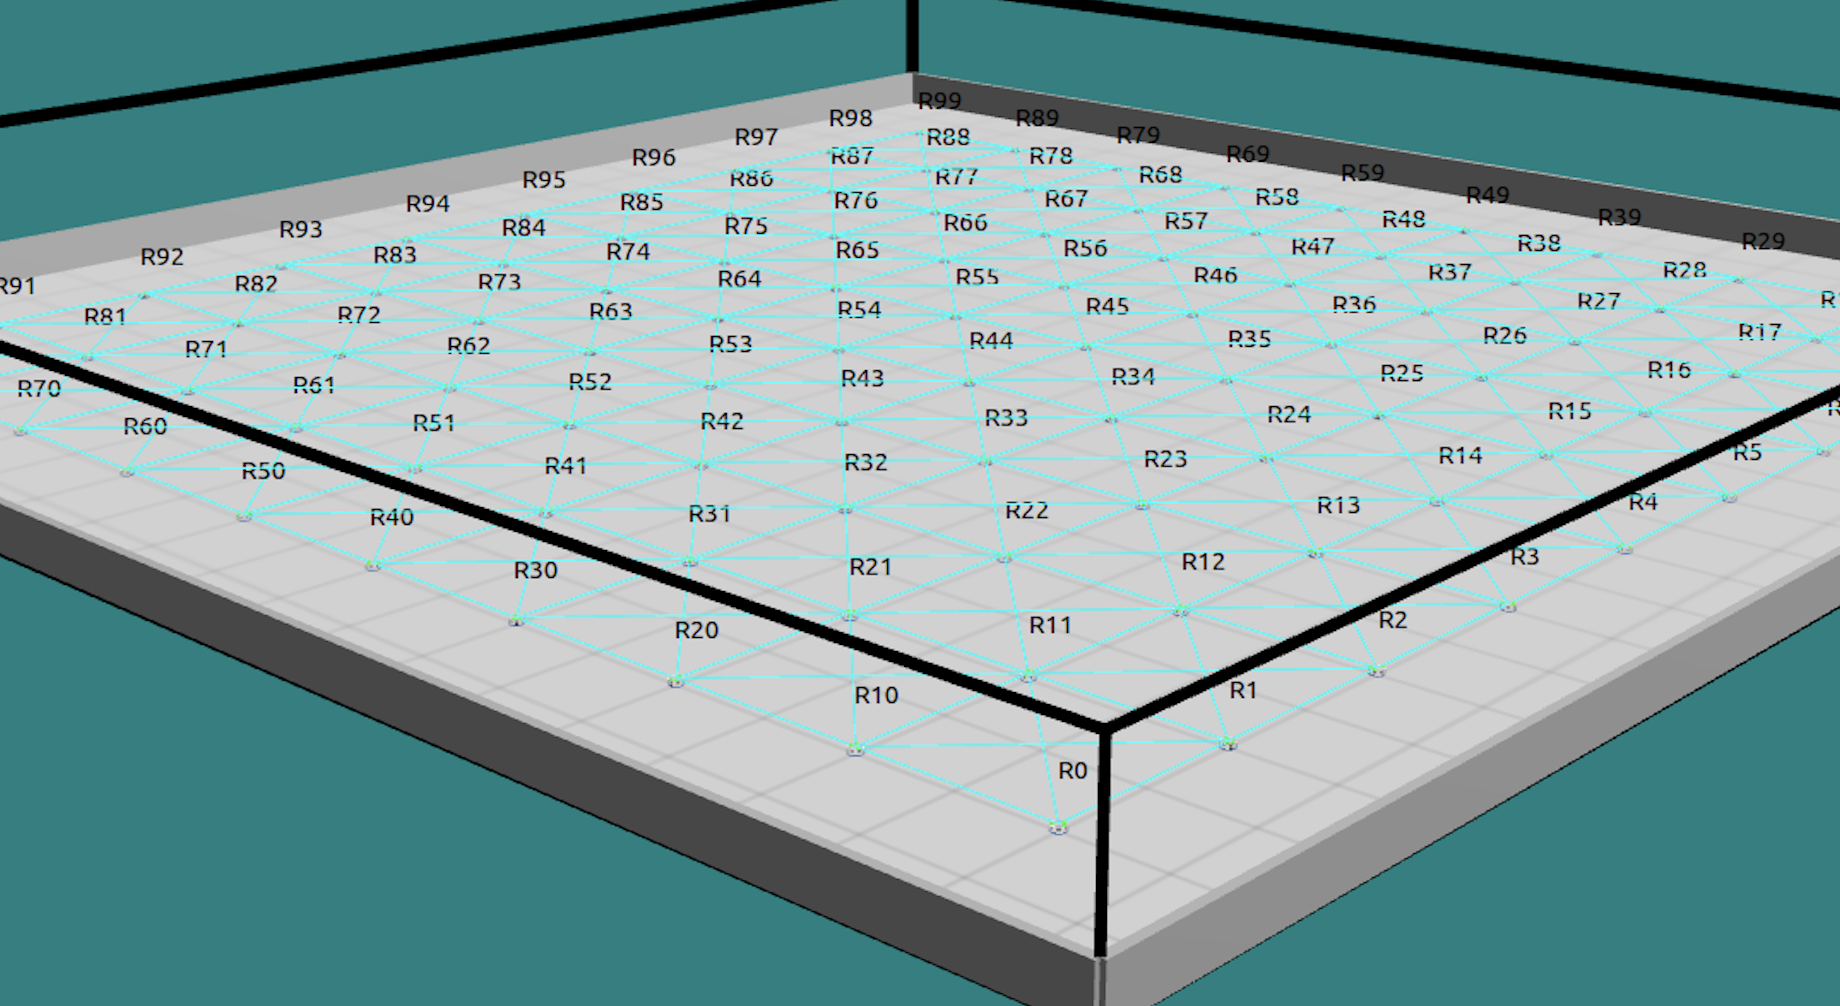
\includegraphics[width=\columnwidth]{figures/dora_mesh/argos_grid_link.png}
    \caption[Grid formation in ARGoS]{$400 \text{m}^2$ environment in the ARGoS simulator with 100 KheperaIV robots distributed in a grid-like pattern.}
    \label{argos:grid}
\end{figure}

\begin{figure}[htbp]
	\centering
    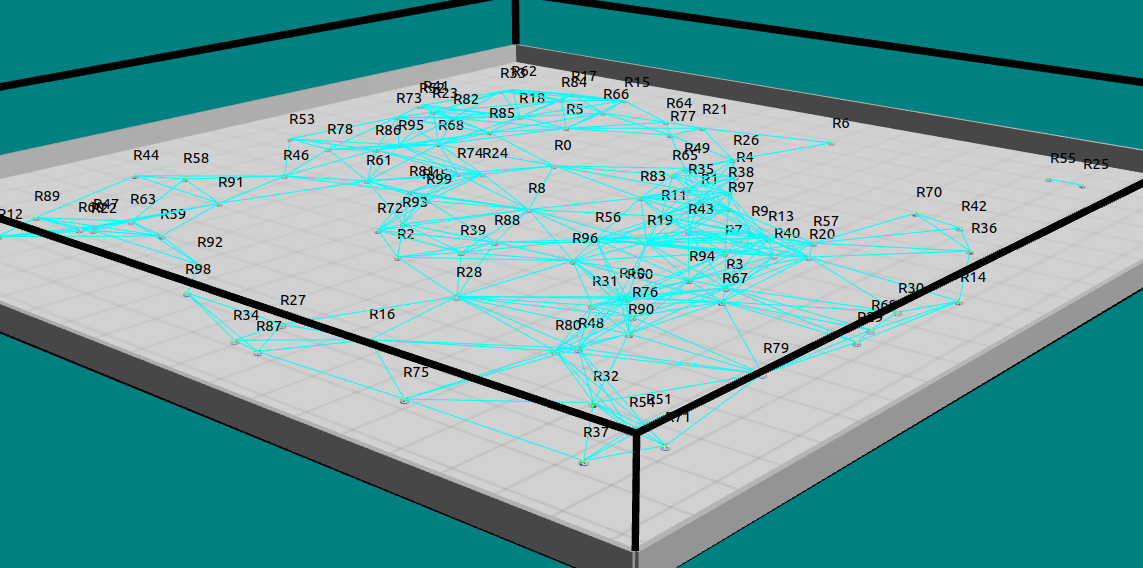
\includegraphics[width=\columnwidth]{figures/dora_mesh/argos_scale_free.png}
    \caption[Scale-free formation in ARGoS]{$400 \text{m}^2$ environment in the ARGoS simulator with 100 KheperaIV robots distributed in a scale-free pattern.}
    \label{argos:scale-free}
\end{figure}

\begin{figure}[htbp]
	\centering
    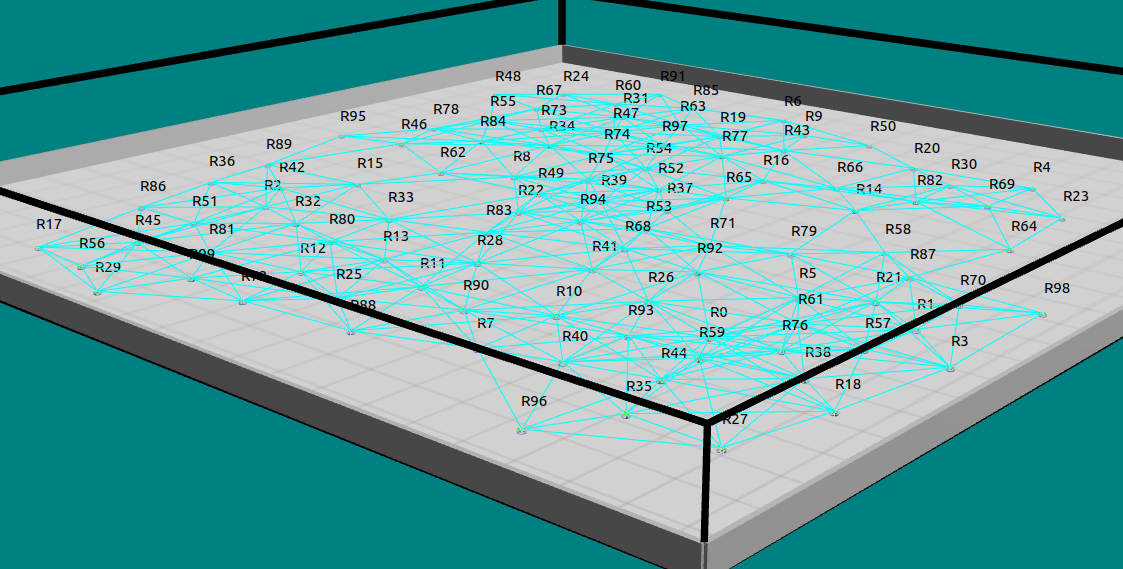
\includegraphics[width=\columnwidth]{figures/dora_mesh/argos_lennard.png}
    \caption[Lennard-Jones potential formation in ARGoS]{$400 \text{m}^2$ environment in the ARGoS simulator with 100 KheperaIV robots in a formation obtained through Lennard-Jones potential interactions.}
    \label{argos:lennard-jones}
\end{figure}

\begin{figure}[htbp]
	\centering
    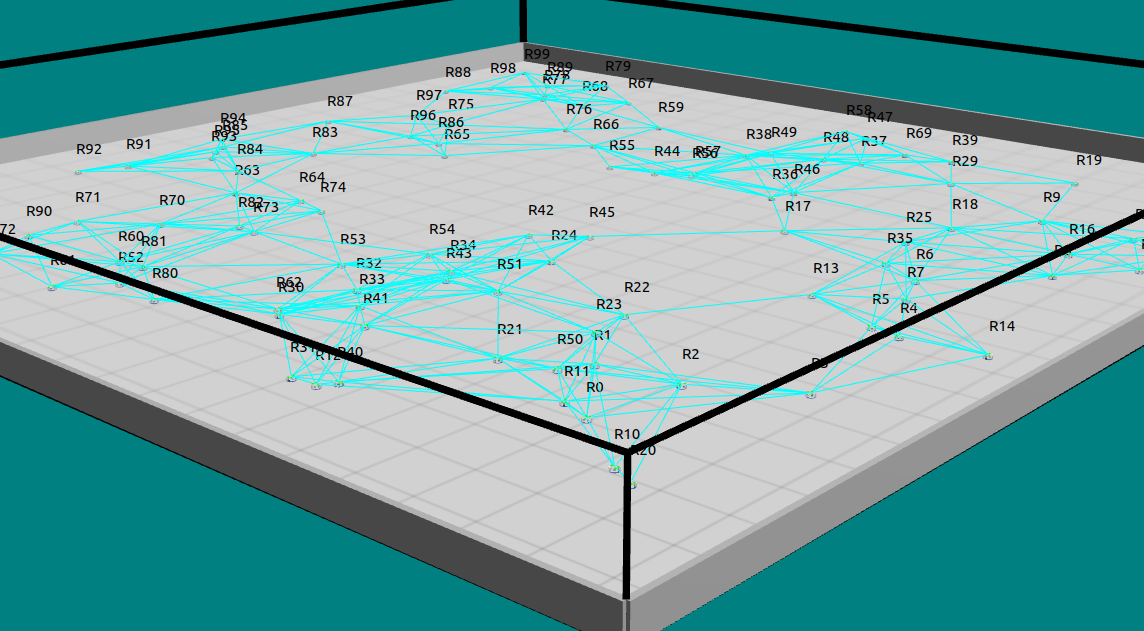
\includegraphics[width=\columnwidth]{figures/dora_mesh/argos_random.png}
    \caption[Random formation in ARGoS]{$400 \text{m}^2$ environment in the ARGoS simulator with 100 KheperaIV robots in a formation obtained through random walk motions.}
    \label{argos:random-walk}
\end{figure}

In order to replicate realistic operation scenarios, we chose to artificially introduce bandwidth limitations. In all experiments, robots can only exchange up to 10 data items at every time step. For the same reason, our simulated robots have a limited storage capacity of 50 data items of at most 50 bytes each, as the data are simple items such as small tables or floating-point numbers. This gives a total storage capacity of 2500kb per robot. Because the robots can only exchange up to 20\% of their stored data at a given time step, it amounts to a bandwidth of 0.5kb/s. Data are generated by each robot at fixed out of phase intervals. 

To evaluate the performance of our system in different scenarios, we tested it with static topologies: a grid-like formation, and a scale-free network; as well as with dynamic topologies: a formation obtained through Lennard-Jones potential interactions and a formation evolving from random walk motions. Testing with static topologies allows us to verify applicability with fixed wireless sensor networks relevant to IoT applications, while experiments with dynamic topologies are more relevant for mobile robotics applications.

To setup \ac{RASS}, we used values of $\alpha = 10$ and $beta = 1$ in Eq. \ref{equation:fitness} because risk measurement values are normalized between 0 and 1 while hop-count values are typically upper-bounded to 10 (for 100 robots). Our first benchmark algorithm is to use a fitness policy based purely on hop count, i.e. if required, data is sent only to neighbours closer to the base station. Our second comparison baseline is to store data in a virtual stigmergy (a \ac{CRDT}) \cite{pinciroliTuple2016}. Using the virtual stigmergy practically ensures that no data can be lost due to corruption because it is fully replicated across the system. The first metric we used in our performance evaluation is the reliability $R$, expressed as:

\begin{equation}
    R = \frac{n_g - n_l}{n_g}
    \label{equation:reliability}
\end{equation}

where $n_g$ and $n_l$ are respectively the amount of data generated and lost at every time step. The second metric is the average data transfer speed, measured as the delay between the creation of a given datum and its arrival by percolation to the base station. We excluded results of this metric for the virtual stigmergy, as the stigmergy cannot include the concept of a base station (since all nodes are peers), and stigmergy propagation speeds are detailed in \cite{pinciroliTuple2016}. The third metric is the evolution of the system's total storage capacity over time, i.e. the amount of data stored by the agents and the base station combined.


\subsection{Results}

The results obtained in the 30 simulation runs for the static topologies (grid-like and scale-free) as well as for the dynamic topologies (Lennard-Jones potential and random walk) are presented by metric in Figs. \ref{results:rass_reliability}, \ref{results:rass_speed} and \ref{results:rass_storage}.

\begin{figure}
    \centering
    \begin{subfigure}{0.45\textwidth}
        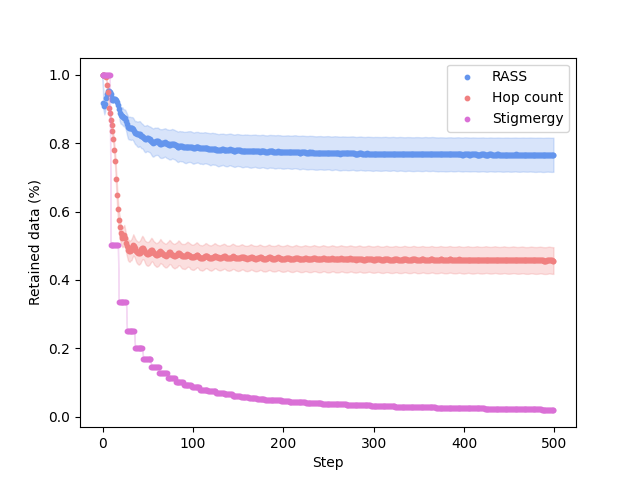
\includegraphics[width=\textwidth]{figures/dora_mesh/grid_reliability.png}
        \caption{Grid topology}
        \label{results:grid_100_reliability}
    \end{subfigure}
    \begin{subfigure}{0.45\textwidth}
        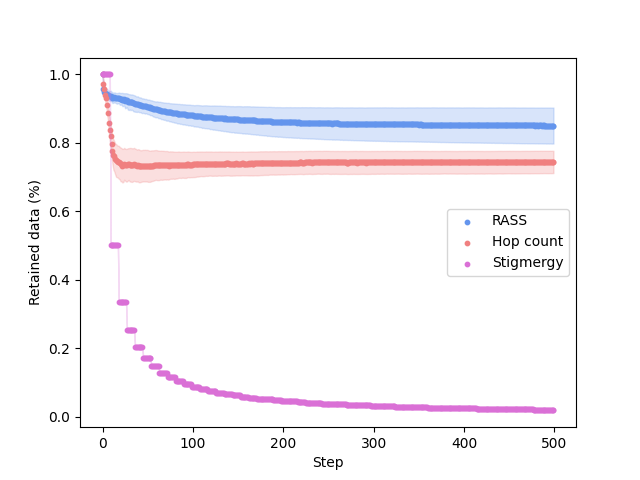
\includegraphics[width=\textwidth]{figures/dora_mesh/scale_reliability.png}
        \caption{Scale-free topology}
        \label{results:scale_100_reliability}
    \end{subfigure}
    \begin{subfigure}{0.45\textwidth}
        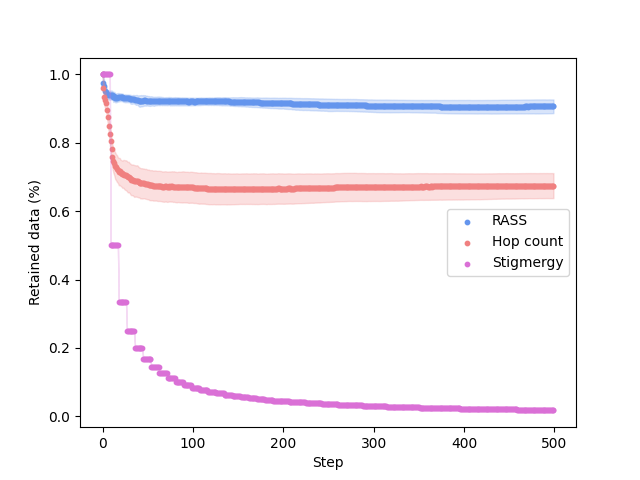
\includegraphics[width=\textwidth]{figures/dora_mesh/lennard_reliability.png}
        \caption{Lennard-Jones topology}
        \label{results:lennard_100_reliability}
    \end{subfigure}
    \begin{subfigure}{0.45\textwidth}
        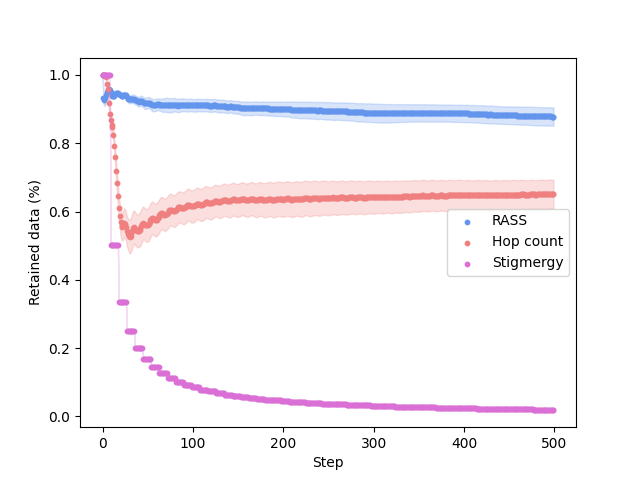
\includegraphics[width=\textwidth]{figures/dora_mesh/random_reliability.png}
        \caption{Random topology}
        \label{results:random_100_reliability}
    \end{subfigure}
    \caption[RASS reliability]{Reliability comparison of \ac{RASS}, hop count and stigmergy in different topologies.}
    \label{results:rass_reliability}
\end{figure}

\begin{figure}
    \centering
    \begin{subfigure}{0.45\textwidth}
        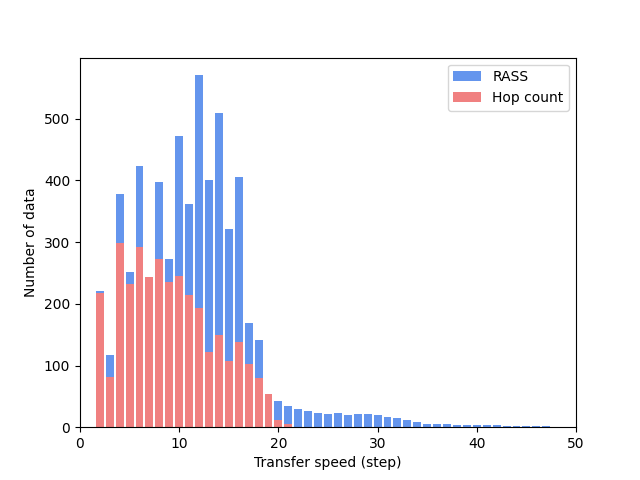
\includegraphics[width=\textwidth]{figures/dora_mesh/grid_speed.png}
        \caption{Grid topology}
        \label{results:grid_100_speed}
    \end{subfigure}
    \begin{subfigure}{0.45\textwidth}
        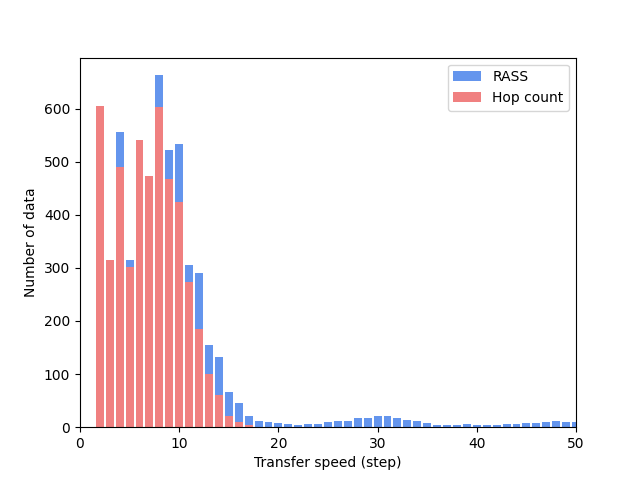
\includegraphics[width=\textwidth]{figures/dora_mesh/scale_speed.png}
        \caption{Scale-free topology}
        \label{results:scale_100_speed}
    \end{subfigure}
    \begin{subfigure}{0.45\textwidth}
        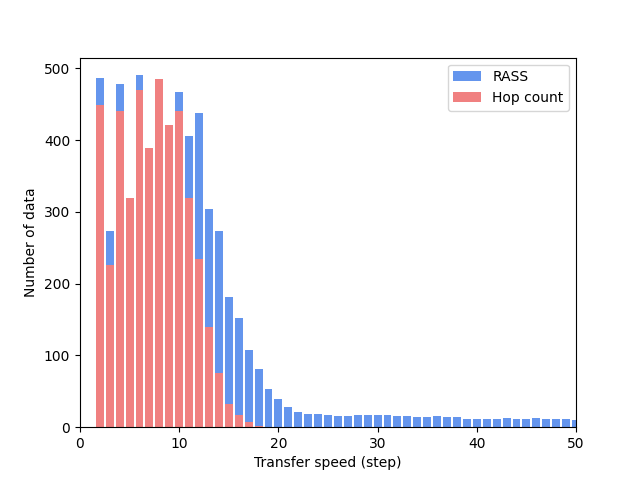
\includegraphics[width=\textwidth]{figures/dora_mesh/lennard_speed.png}
        \caption{Lennard-Jones topology}
        \label{results:lennard_100_speed}
    \end{subfigure}
    \begin{subfigure}{0.45\textwidth}
        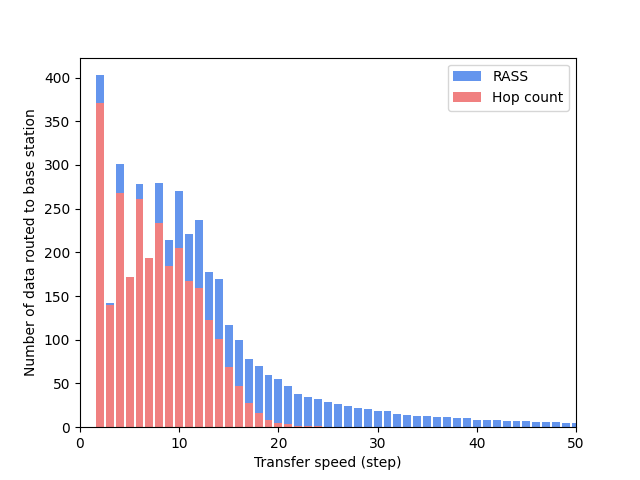
\includegraphics[width=\textwidth]{figures/dora_mesh/random_speed.png}
        \caption{Random topology}
        \label{results:random_100_speed}
    \end{subfigure}
    \caption[RASS transfer speeds]{Speed comparison of \ac{RASS}, hop count and stigmergy in different topologies.}
    \label{results:rass_speed}
\end{figure}

\begin{figure}
    \centering
    \begin{subfigure}{0.45\textwidth}
        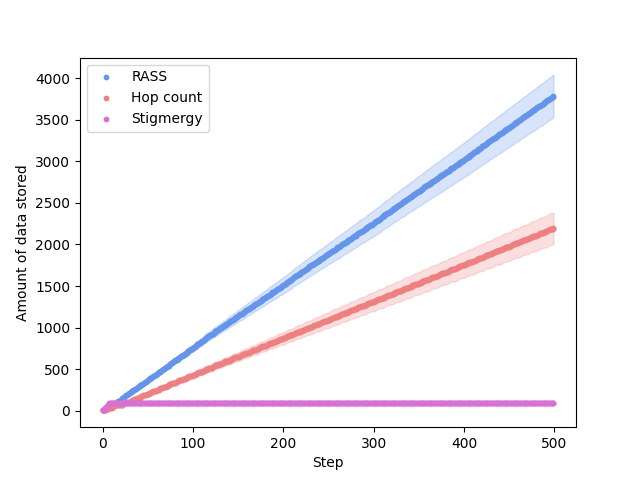
\includegraphics[width=\textwidth]{figures/dora_mesh/grid_storage.png}
        \caption{Grid topology}
        \label{results:grid_100_storage}
    \end{subfigure}
    \begin{subfigure}{0.45\textwidth}
        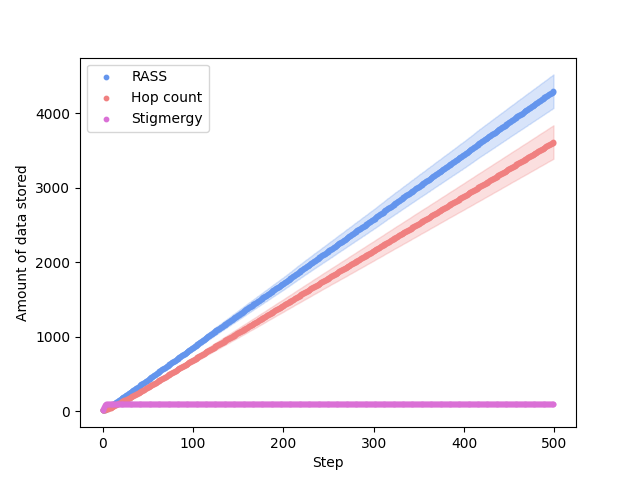
\includegraphics[width=\textwidth]{figures/dora_mesh/scale_storage.png}
        \caption{Scale-free topology}
        \label{results:scale_100_storage}
    \end{subfigure}
    \begin{subfigure}{0.45\textwidth}
        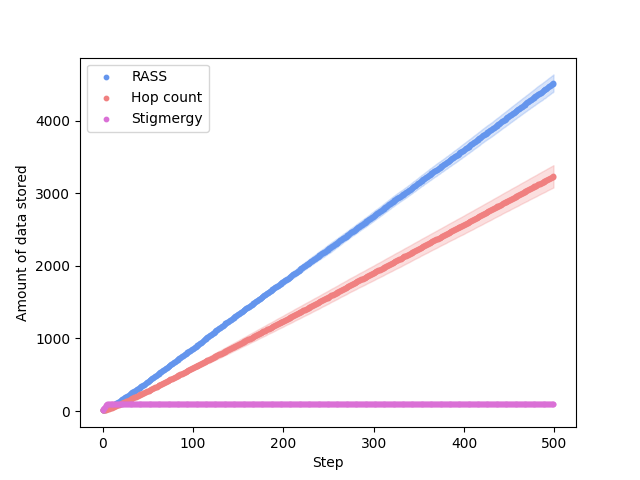
\includegraphics[width=\textwidth]{figures/dora_mesh/lennard_storage.png}
        \caption{Lennard-Jones topology}
        \label{results:lennard_100_storage}
    \end{subfigure}
    \begin{subfigure}{0.45\textwidth}
        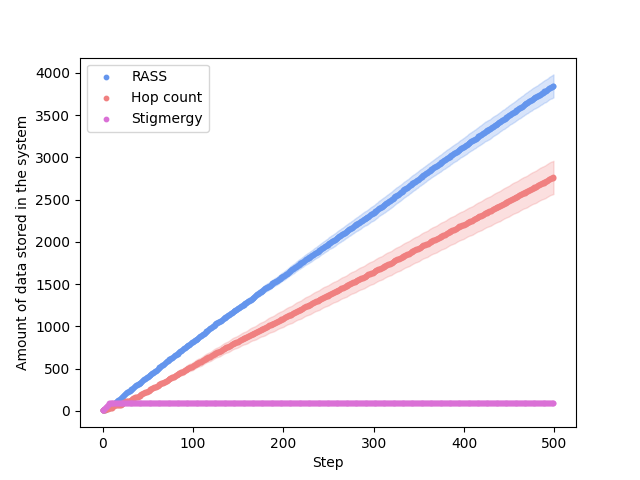
\includegraphics[width=\textwidth]{figures/dora_mesh/random_storage.png}
        \caption{Random topology}
        \label{results:random_100_storage}
    \end{subfigure}
    \caption[RASS total storage]{Total storage capacity comparison of \ac{RASS}, hop count and stigmergy in different topologies.}
    \label{results:rass_storage}
\end{figure}

Results show that \ac{RASS} outperforms the hop-count algorithm in terms of reliability. Because 
of the risk awareness component included in its fitness policy as detailed in Eq. 
\ref{equation:fitness}, robots do not always route the data through the shortest path to 
the base station. \ac{RASS} avoids the dangerous storage nodes of the system when routing data 
which explains the higher reliability levels displayed in Fig. 
\ref{results:grid_100_reliability}, Fig. \ref{results:scale_100_reliability}, Fig. 
\ref{results:lennard_100_reliability} and Fig. \ref{results:random_100_reliability} . This 
is why, on average, \ac{RASS} takes 54.89\% more time to route the data to the base station when 
compared to the hop-count algorithm. The shortest path might not always be the safest one; 
\ac{RASS} will take an alternate route if the risk associated with the shortest one is too high. 
On the other hand, the hop-count algorithm always takes the shortest path towards the base 
station regardless of the risk associated with it. This leads to a higher number of data 
losses due to corruption and an overall lower reliability.
However, hop count can yield faster transfer speeds as shown in Fig. \ref{results:grid_100_speed}, Fig. \ref{results:scale_100_speed}, Fig. \ref{results:lennard_100_speed}, Fig. \ref{results:random_100_speed} and table \ref{table:speed}.

\begin{table}[htbp]
\centering
\caption[RASS performance summary for different topologies]{Average transfer speed and average individual memory usage with different topologies.}

\begin{tabular}{|l|l|c|c|}
\hline\rowcolor[gray]{0.8}\color{black}
\textit{Topology} & \textit{Algorithm} & \textit{Transfer speed (hops)} & \textit{Memory used  (\%)} \\ \hline
\multirow{3}{*}{Grid-like}            & \ac{RASS}                                   & 11.45                                                                     & 1.35                                                                 \\
                                      & Hop-Count                              & 9.11                                                                      & 0.61                                                                 \\
                                      & Stigmergy                              & N.A.                                                                      & 100.00                                                               \\ \hline
\multirow{3}{*}{Scale Free}           & \ac{RASS}                                   & 11.44                                                                     & 1.95                                                                 \\
                                      & Hop-Count                              & 6.85                                                                      & 0.50                                                                 \\
                                      & Stigmergy                              & N.A.                                                                      & 100.00                                                               \\ \hline
\multirow{3}{*}{Lennard-Jones}        & \ac{RASS}                                   & 12.51                                                                     & 1.69                                                                 \\
                                      & Hop-Count                              & 7.32                                                                      & 0.51                                                                 \\
                                      & Stigmergy                              & N.A.                                                                      & 100.00                                                               \\ \hline
\multirow{3}{*}{Random search}        & \ac{RASS}                                   & 12.68                                                                     & 1.67                                                                 \\
                                      & Hop-Count                              & 7.76                                                                      & 0.57                                                                 \\
                                      & Stigmergy                              & N.A.                                                                      & 100.00                                                               \\
\hline
\end{tabular}
\label{table:speed}
\end{table}

For the virtual stigmergy, most of the data losses can be attributed to the storage having reached its maximum capacity. Indeed, because of the fully replicated nature of the stigmergy, the memory of the agents is quickly saturated. Table \ref{table:speed} shows that on average, across the 500 steps of the simulations runs, the virtual stigmergy has 100\% of every individual robot memory used. This means that the nodes of the system are simply full and cannot store data anymore. In comparison, \ac{RASS} uses between 1\% and 2\% of the local memories of the nodes, and hop-count is even lower at values around 0.5\%. This full redundancy prevents losing data from corruptions. However, it entails a very inefficient use of the memory of the robots and ultimately leads to data losses due to insufficient memory capacity. The result is an unchanging storage capacity over time and poor reliability as shown in Fig. \ref{results:grid_100_reliability} for the virtual stigmergy strategy.

The low values of local memory usage shown in Table \ref{table:speed} for \ac{RASS} and hop-count were obtained because the topologies used to test the algorithms were usually well connected in accordance with the connected graph assumption we made in \ref{section:routingTable}. For the most part, multiple routes were connecting the nodes to the base station and as a result, the collected data was routed towards the base station instead of being kept locally. Such a result implies that the system, by maintaining a low individual storage occupancy, allows the robot to adapt to situations in which they would be temporarily stranded: if their storage were to be mostly full, they would not be able to generate new data without promptly losing it. This storage buffer thus allows them to continue their data collection while they are temporarily disconnected from the rest of the swarm.

\section{Physical experiments}
\label{Physical experiments}

\subsection{Experimental setup}
We evaluated \ac{RASS}' performance with the same
metrics on physical robots to confirm the real-world applicability of our system. We used 5 small drones in a controlled indoor environment. These drones use standard Raspberry Pi Zeros as their main computer, meaning they have relatively low capabilities, and are therefore well suited to verify our algorithm. We designed a static topology with one drone acting as a base station and 4 others acting as agents. The radiation source (red cone) in Fig. \ref{cogniflyExperiment} is positioned to make one of the paths more dangerous, allowing us to verify if data is routed in the longer but safer path. The communication range is set to 1.5m. The topology is illustrated in Fig. \ref{cogniflyExperiment}. To assess \ac{RASS}' performance, we compared it with a hop-count algorithm over 3 runs.

\begin{figure}[htbp]
	\centering
    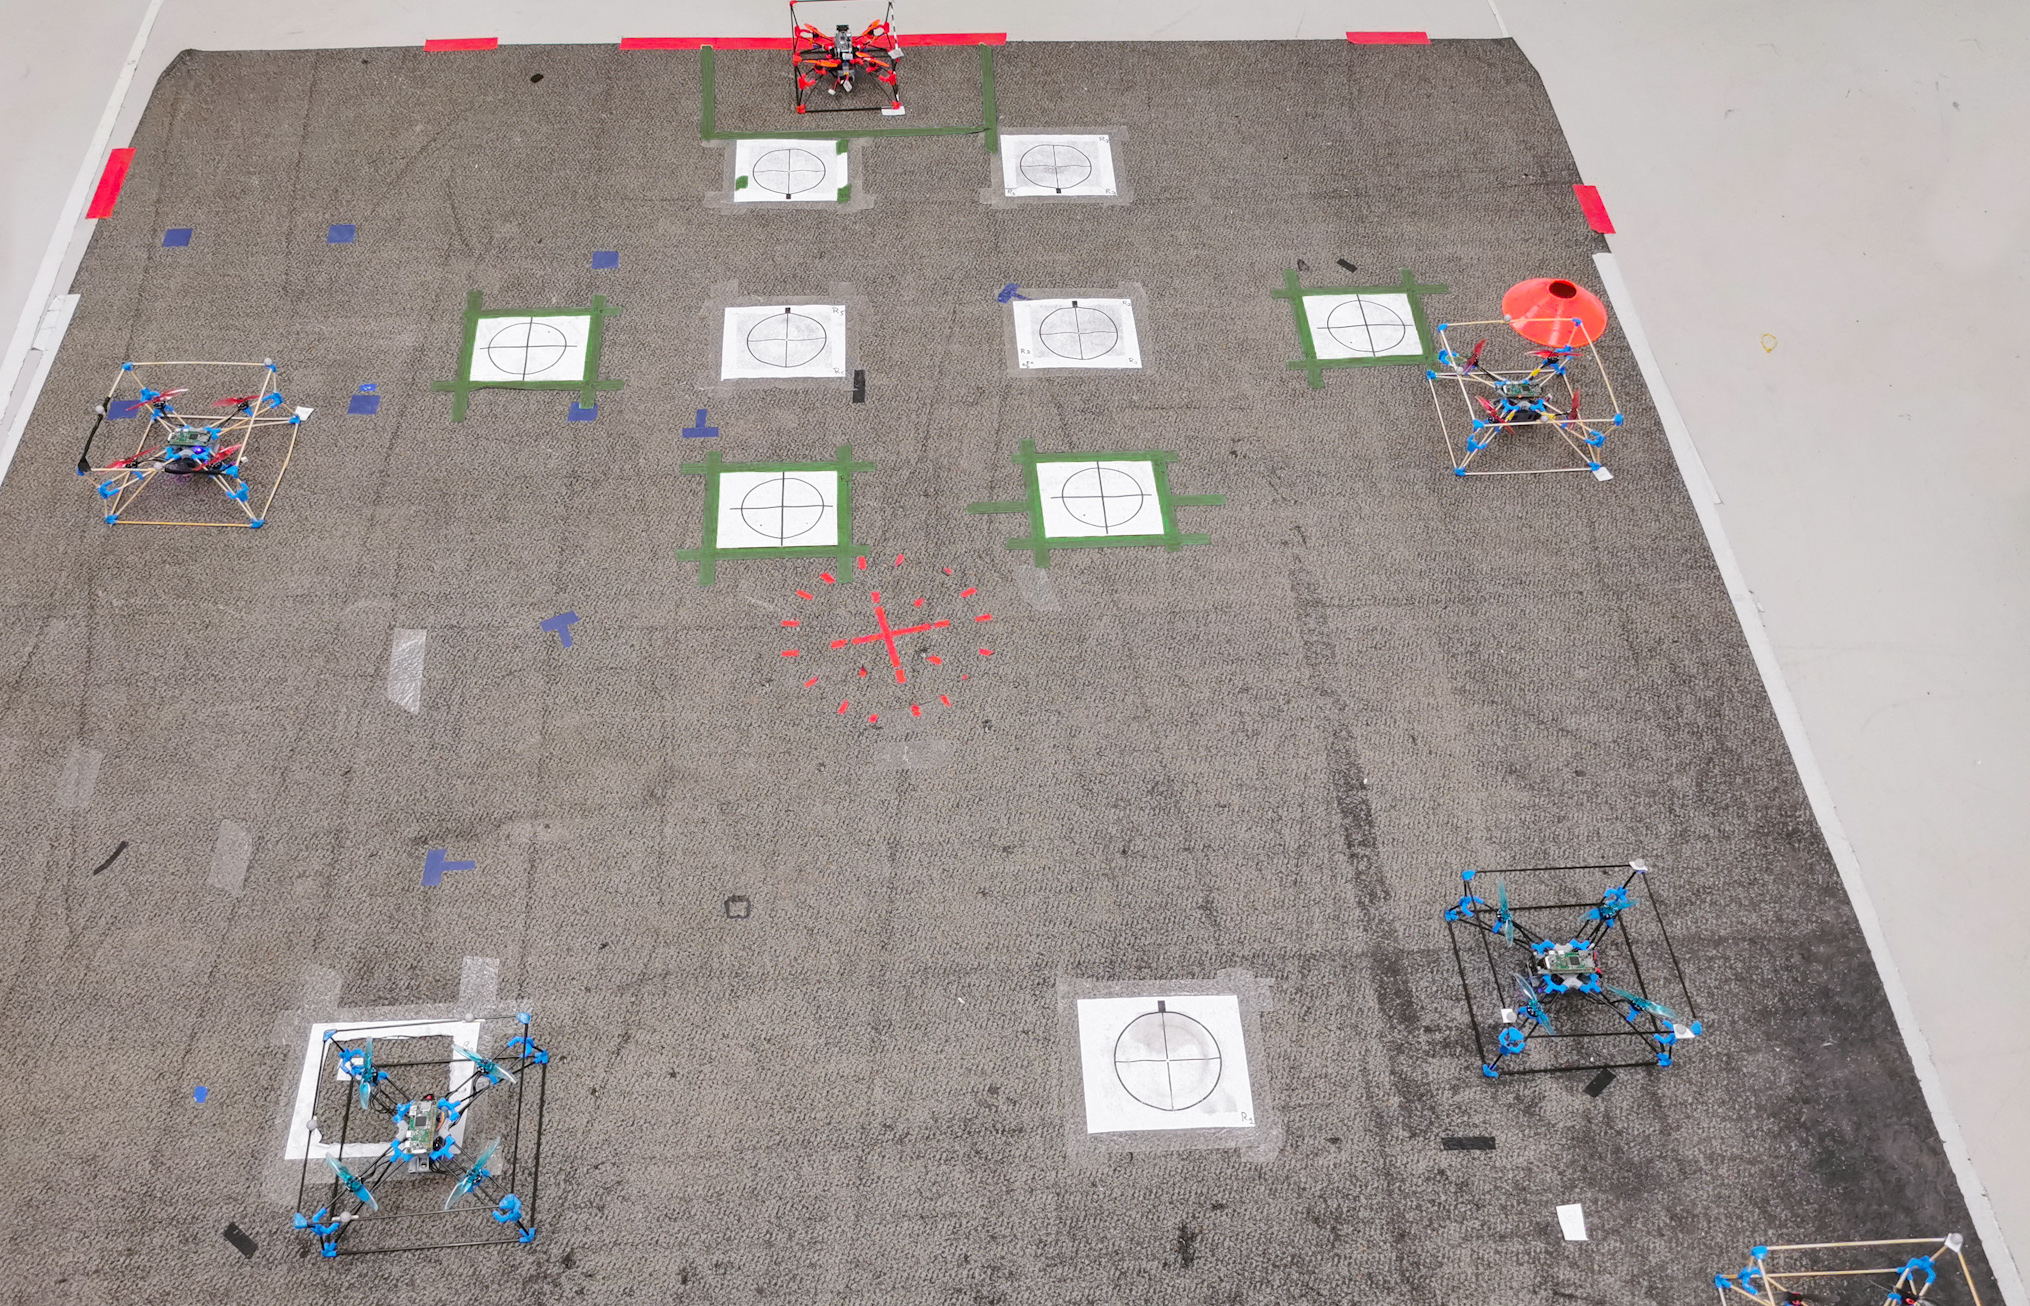
\includegraphics[width=\columnwidth]{figures/dora_mesh/cognifly.jpg}
    \caption[RASS physical experiment setup]{3x3m environment with 5 drones and a radiation source (red cone).}
    \label{cogniflyExperiment}
\end{figure}

\subsection{Results}
The reliability results of the physical experiments conducted on the drones are presented in Fig. \ref{results:physicalRelaibility}. They show that \ac{RASS} outperforms the hop-count algorithm in terms of reliability which lead to overall greater swarm storage. Even if the topology used to assess the performance of our algorithm was simple and the number of agents in the system was limited, the physical experiments confirm the real-world applicability of \ac{RASS}. Using only local interactions, it was able to choose safer paths for the data to be routed through which resulted in fewer data corruptions.

\begin{figure}[htbp]
	\centering
    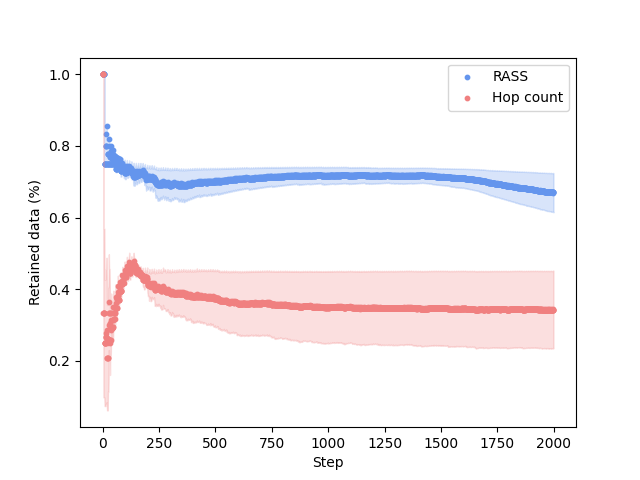
\includegraphics[width=\columnwidth]{figures/dora_mesh/reliability.png}
    \caption[RASS physical reliability]{Evolution of reliability over time on the the physical experiments}
    \label{results:physicalRelaibility}
\end{figure}

\section{Conclusions}
\label{conclusion}

We presented \ac{RASS}, a Risk-Aware Swarm Storage system in which a swarm of robots can collectively store data on strategically chosen members. This choice is made without central coordination and is purely based on local information shared between the robots. This information is simply composed of risk measurements and topological distance from a robot to a base station, and a used to determine a robot's fitness to store data as well as to establish the most reliable and fast route towards the base station.

We show in our experiments that \ac{RASS} largely outperforms a hop-count-based solution as well as a virtual stigmergy in terms of reliability and total swarm storage capacity, while only being slightly slower in terms of percolation speed compared to the hop-count-based algorithm. \ac{RASS} showed good scalability in physics-based experiments as it repeatedly performed well with a large number of robots. It also performed well in experiments on physical robots.

 A possible improvement for the system could be to use a Kalman Filter \cite{kalman1960new} to eliminate outliers in radiation measurement which can arise due to sensor imprecision. More generally, an interesting direction for future work could be to conduct experiments in more diverse scenarios, for example in search and rescue applications where image storage and processing is required, therefore increasing the system's workload.
             % Premier thème (Doctorat) ou "Détails de la Solution" (Maîtrise).
\Chapter{Risk Aware Exploration}\label{sec:Theme2}

In this chapter, I describe my contribution to an article on which I worked, \ac{DORA} \cite{vielfaure2021dora}, which is closely related to the theme of risk awareness in swarm robotics. Figures in this chapter are taken from the article with permission from the authors.

Because exploration of unknown environments is an important challenge in the
field of robotics, we wanted to show the benefits of taking risk awareness into account when developing solutions for this kind of challenge. We based our exploration strategy on distributed belief maps. This way, swarm efficiency is leveraged because robots collaborate by sharing useful information. The key idea behind \ac{DORA} is to minimize risk exposure while maximizing exploration coverage, leading to more efficient exploration because of fewer risk-related failures. 


\section{Introduction}
Unknown environment exploration by robots has applications in numerous fields. For example, search-and-rescue missions \cite{matos2016multiple} and space missions \cite{fong2005interaction} can both benefit from using robots, as they often operate in environments inaccessible to humans. This inaccessibility can stem from multiple causes, such as the remote nature of these places (space, other planets, oceanic depths), the impossibility for humans to reach them (grottoes with too small openings) or their dangerous nature (radioactive zones, forest fires, flooded areas). For all of these, there is necessarily an associated risk factor, which means that robots sent to explore them will necessarily be exposed to some danger increasing the risk of failures. Robot swarms mitigate the effects of individual failures ~\cite{ramachandran2019resilience,wehbe2021probabilistic,winfield2006safety} and improve overall terrain coverage performance \cite{burgard2005coordinated}. However, even in robot teams, failures have negative effects on overall performance, which is why we sought to reduce them as much as possible through \ac{DORA}.

The motivation for creating a purely decentralized algorithm is to avoid the pitfalls related to centralized systems, such as bottlenecks and single points of failures. The first can be related to low capacity robots, or to noisy environments affecting communication efficiency or causing memory corruption. The second is particularly important in the risky scenarios where individual malfunctions are more likely and could cause system-wide failures. Consequently, relying on locally shared information and onboard computation is necessary.

As we found no existing decentralized risk-aware exploration algorithm, we sought to create one.


% \section{Related Work and Background}
% Distributed information sharing is not trivial, especially considering
% the challenges of consistency and partial connectivity among the
% robotic teams~\cite{amigoni2017multirobot}. The virtual stigmergy
% presented in \cite{pinciroliTuple2016} and implemented in the Buzz
% programming language \cite{pinciroliBuzz2016} achieves consensus among
% a group of robots using \ac{CRDT}s,
% represented as key-value pairs. This sort of shared data structure is
% particularly relevant for belief maps, since it is easy to assign a
% unique key to each cell based on its location.  In the virtual
% stigmergy, data is shared on writing and reading the \ac{CRDT}, with the
% additional updates on read improving the robustness to temporary
% disconnections and message drops. This solution differs from
% distributed hash tables, which require a complete view of the system
% at every point in time. Other distributed data storage approaches such
% as SwarmMesh \cite{majcherczykSwarmmesh2020} store data in different
% locations based on a fitness function instead of replicating them on
% all robots. This allows the storage of more data with less
% communication, but robots are less likely to have access to the latest
% values.

% Belief maps are a simple yet powerful tool for robotic exploration
% because they can represent an environment with a 2D cell grid. They
% are a generalization of occupancy maps: instead of storing only one
% bit per cell to indicate the presence of an obstacle/danger, they
% store obstacle/danger likelihoods and offer significant improvements
% for exploration \cite{stachnissMappingExplorationMobile2003}. In the
% field of multi-robot exploration, early techniques leveraging belief
% maps date back as far as twenty years
% \cite{kobayashiSharingExploringInformation2002,kobayashiDeterminationExplorationTarget2003},
% but they rely on a fixed grid size and are tested only with two
% robots. More recent works also leverage belief maps for multi-robot
% exploration. For example,
% in~\cite{indelmanCooperativeMultirobotBelief2018}, the robots consider
% both the current beliefs and the expected beliefs from future
% observations to coordinate their exploration. Grid maps and belief
% maps are also widely used to train deep reinforcement learning
% exploration policies
% \cite{hanGridWiseControlMultiAgent,panovGridPathPlanning2018}. Such
% techniques generally achieve the best performance in simulated
% environments, but are usually brittle in more realistic and noisy
% scenarios.

% Several path planners based on Markov Decision Processes
% \cite{undurti2010online,thiebaux2016rao,xiao2020robot} take into
% account risk and have useful definitions of it. However, they assume a
% knowledge of the global state of the environment, which is unavailable
% when exploring unknown environments. Furthermore, they are so far only
% applied to single-robot systems.

% Many distributed exploration strategies that maximize the amount of
% covered terrain have been proposed. The first approaches to stand out
% in this regard are Voronoi-based coverage control
% techniques~\cite{luo2019voronoi,santos2019decentralized}. A second
% method covers time-varying domains, in which points of interest in the
% covered region can become more or less interesting to explore,
% therefore prompting a change in the coverage function
% \cite{santos2019decentralized,xu2019multi}. Another method to optimize
% coverage is \ac{FBE}
% \cite{yamauchi1998frontier} of which many variations have been
% developed, such as those based on Particle Swarm Optimization
% \cite{wang2011frontier} or the Wavefront Frontier Detector
% \cite{topiwala2018frontier}. However, none of these strategies take
% risk into account, which is inherent to exploration.  Therefore, the
% exploration strategy implemented in this paper takes inspiration of
% the multi-robot control algorithm presented in
% \cite{dames2012decentralized,schwagerMultirobotControlPolicy2017}
% which maximizes the information gain during exploration in the
% presence of unknown hazards. However, this optimal algorithm has a
% very high computational complexity. In \ac{DORA}-Explorer, we introduce
% approximations to lower the computation load onboard the robots which
% makes it is well suited for real deployment on resource constrained
% robotic platforms.

% We build on those approaches and address some their shortcomings by
% implementing a risk-aware exploration algorithm leveraging a \ac{DBM} of
% the environment which is not constrained to a fixed size.

\section{System Model}
\label{dora_system_model}

The motivation for including risk awareness in a distributed exploration algorithm can be seen in Fig. \ref{risk_unaware}, where failures lead to decreasing performance over time. Conversely, in Fig. \ref{risk_aware}, avoiding dangerous areas reduces failures and maintains exploration efficiency. In order to design our system, we modelled the environment as a 2D grid ($E \subset \mathbb{Z}^2$) in which agents $a_i \in A$ carry out their task. Several design considerations shaped \ac{DORA}. They are summarized here, and more details can be found in the referenced paper.

\FloatBarrier

First, risk and failure probability had to be formally modelled. We chose to represent risk as point radiation sources $s_j \in S$ with an exponentially decaying intensity $I_j$, but any other type of danger could have been used with our system. The equations representing the radiation perceived by a robot $a_i$ failing due to radiation in cell $\bm{x}_i$ can be combined as:

\begin{equation}
    r(\bm{x}_i) = b + \sum_{\bm{s}_j \in S} \frac{I_j}{1 + \lambda\rho_j^2}
    \label{eq:radiation_dora}
\end{equation}

Where $\rho_j$ is the distance between $a_i$ and $s_j$, $\lambda$ is a decay constant and $b$ is Gaussian noise. The probability of failure necessarily increases where $r(\bm{x}_i)$ is higher.

Second, we defined the objective of exploration as gaining information by visiting cells from $E$. Logically, recently visited cells are unlikely to yield any information gain. Therefore, priority is given to unvisited and less recently visited cells. Doing so requires saving the last time of exploration of $\bm{x}_i$ in a scalar field $\epsilon(\bm{x}_i) = t_\epsilon$. The probability of finding useful information decreases exponentially for values of $\epsilon(\bm{x}_i)$ which are closer to the current time step $t$.

Third, as way of storing these values, we use a \ac{CRDT}: the virtual stigmergy from \cite{pinciroliTuple2016}. This allows robots to exchange information whenever possible (thereby achieving a loose eventual consistency) without relying on a central communication hub. Both $r(\bm{x}_i)$ and $\epsilon(\bm{x}_i)$ are stored in distributed belief maps. These are updated at every time step.

Fourth, we describe a position-based control law for the robots which minimize risk and maximize information gain. These optimizations are described by local gradients of each scalar field in a Moore neighborhood (see Fig. \ref{neighborhood}) around $a_i$.

\begin{figure}[htbp]
	\centering
    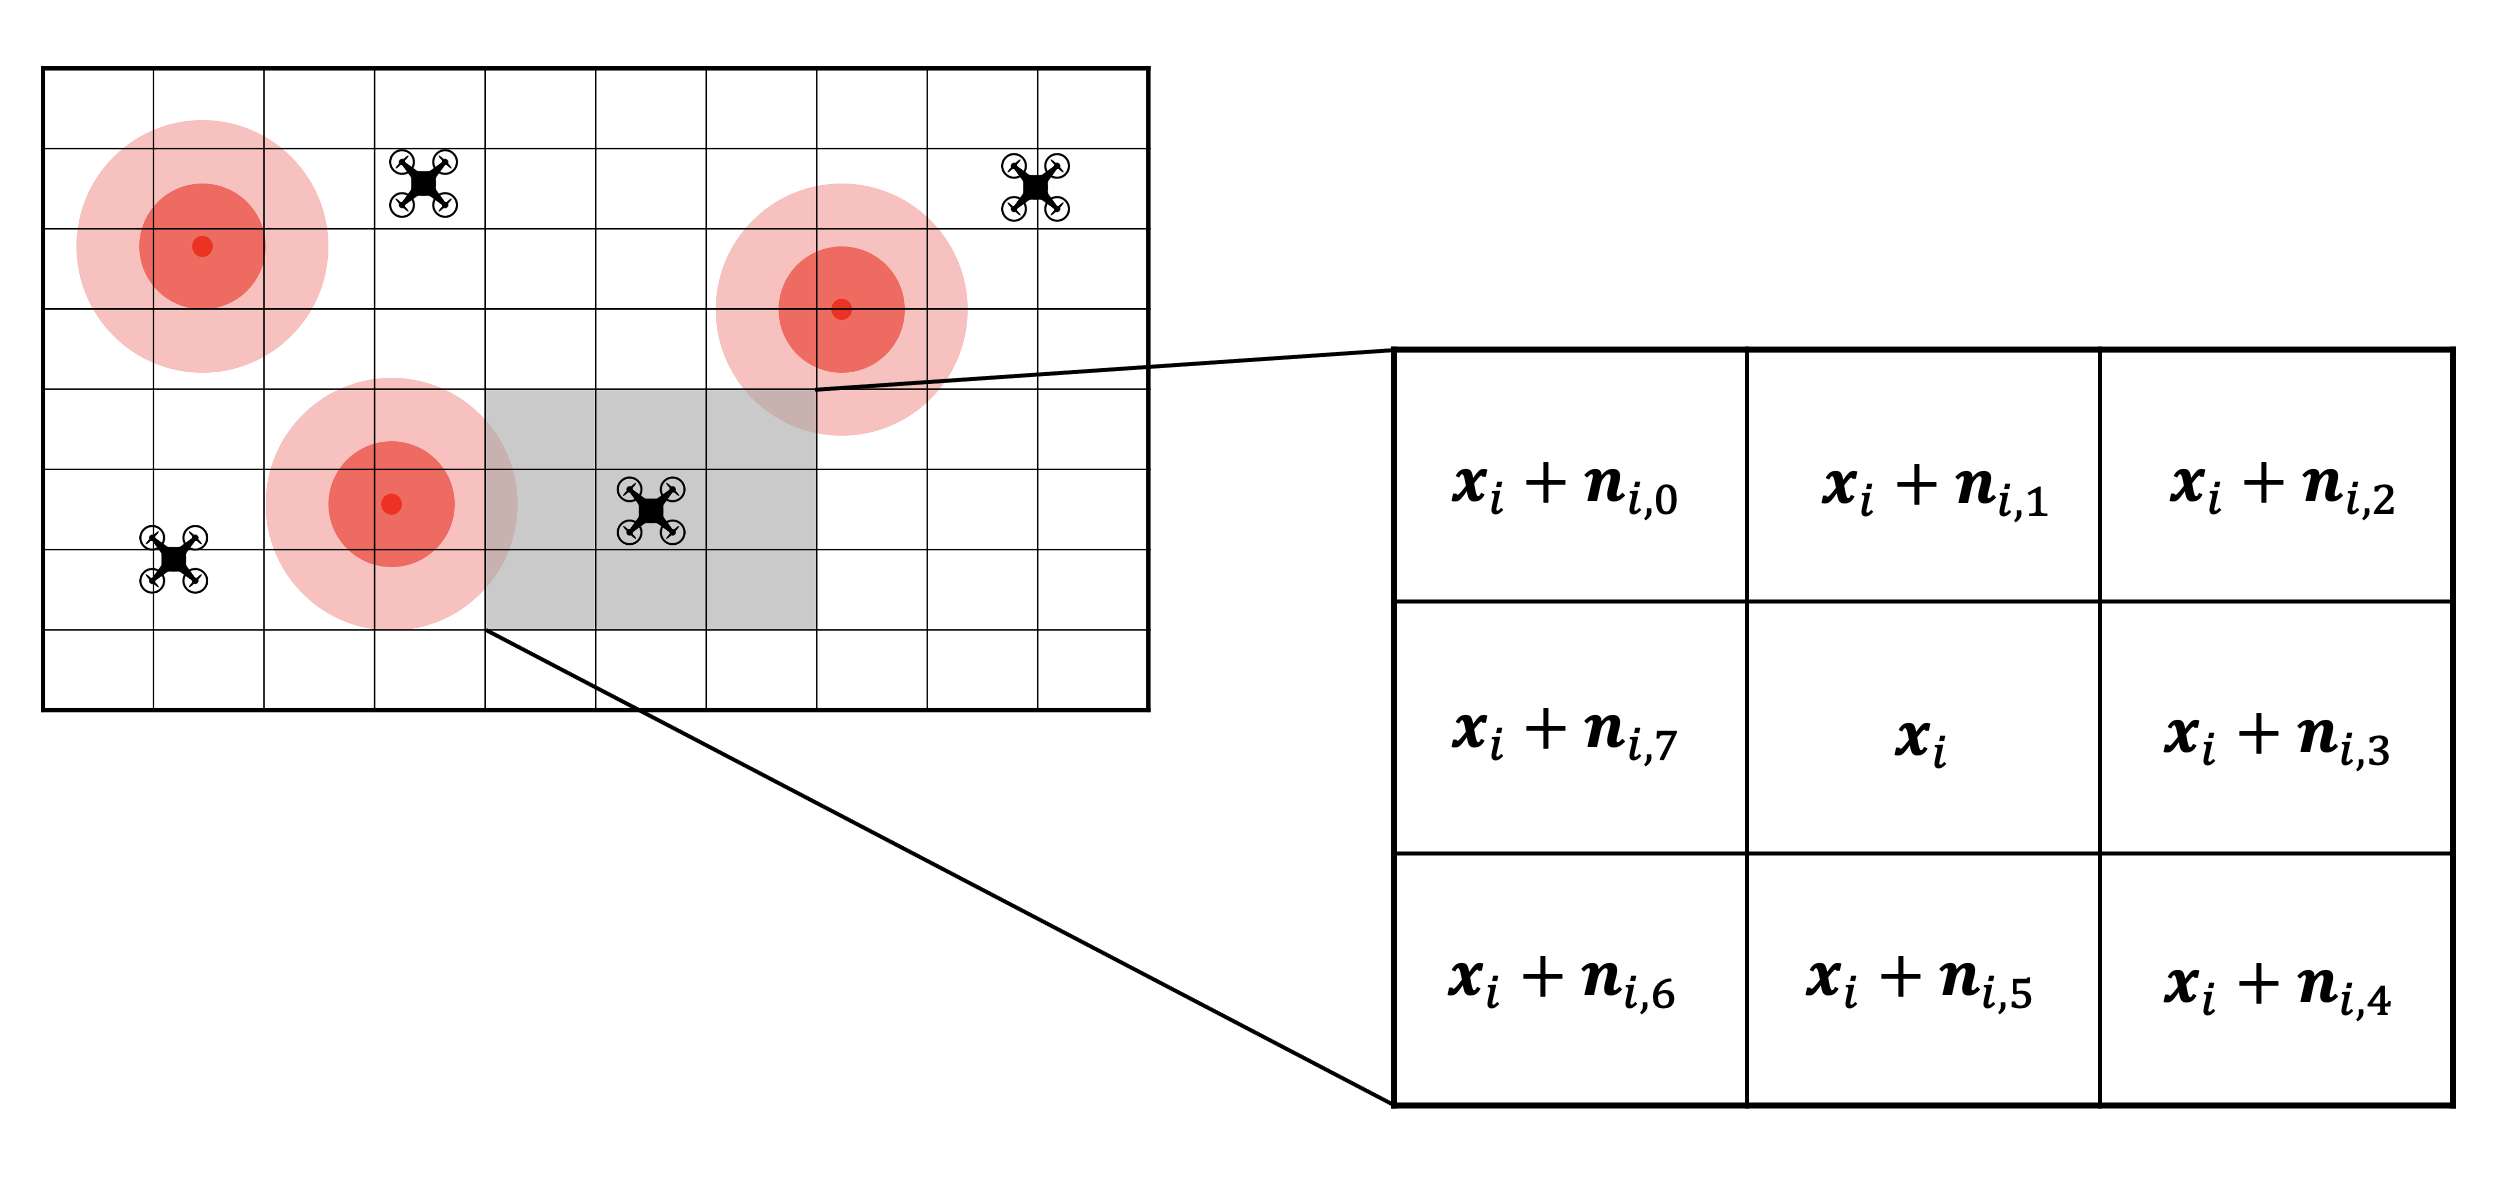
\includegraphics[width=0.95\columnwidth]{figures/dora_explorer/Moore.png}
    \caption[Moore neighborhood]{$\bm{x}_i$'s neighborhood. $\bm{n}_{i,0} = (-1, 1)$ is neighbor 0's offset from $\bm{x}_i$.}
    \label{neighborhood}
\end{figure}

The risk gradient $\bm{\nabla}_{r;i}$ is given by:

\begin{equation}
    \bm{\nabla}_{r;i} = \sum_{\bm{n}_j \in \nu}\bm{\hat{n}}_{i,j} \cdot (r(\bm{x}_i) - r(\bm{n}_{i,j}))
    \label{eq:gradient}
\end{equation}

where $\bm{\hat{n}}$ is the unit form of $\bm{n}$. The exploration gradient $\bm{\nabla}_{\epsilon;i}$ is calculated in the same manner. We combine these to obtain the control law:

\begin{equation}
    \bm{x}_i^{t+1} = \bm{x}_i^t + (\alpha\bm{\nabla}_{r;i} + \beta\bm{\nabla}_{\epsilon;i} + \gamma\bm{o}_i)
    \label{eq:control_law}
\end{equation}

where $\alpha, \beta, \gamma$ are parameters related to risk avoidance, exploration gain and obstacle avoidance control. The latter is added from robustness and inspired from \cite{shahriari2018lightweight}.

\begin{figure*}
     \centering
     \begin{subfigure}{0.45\textwidth}
         \centering
         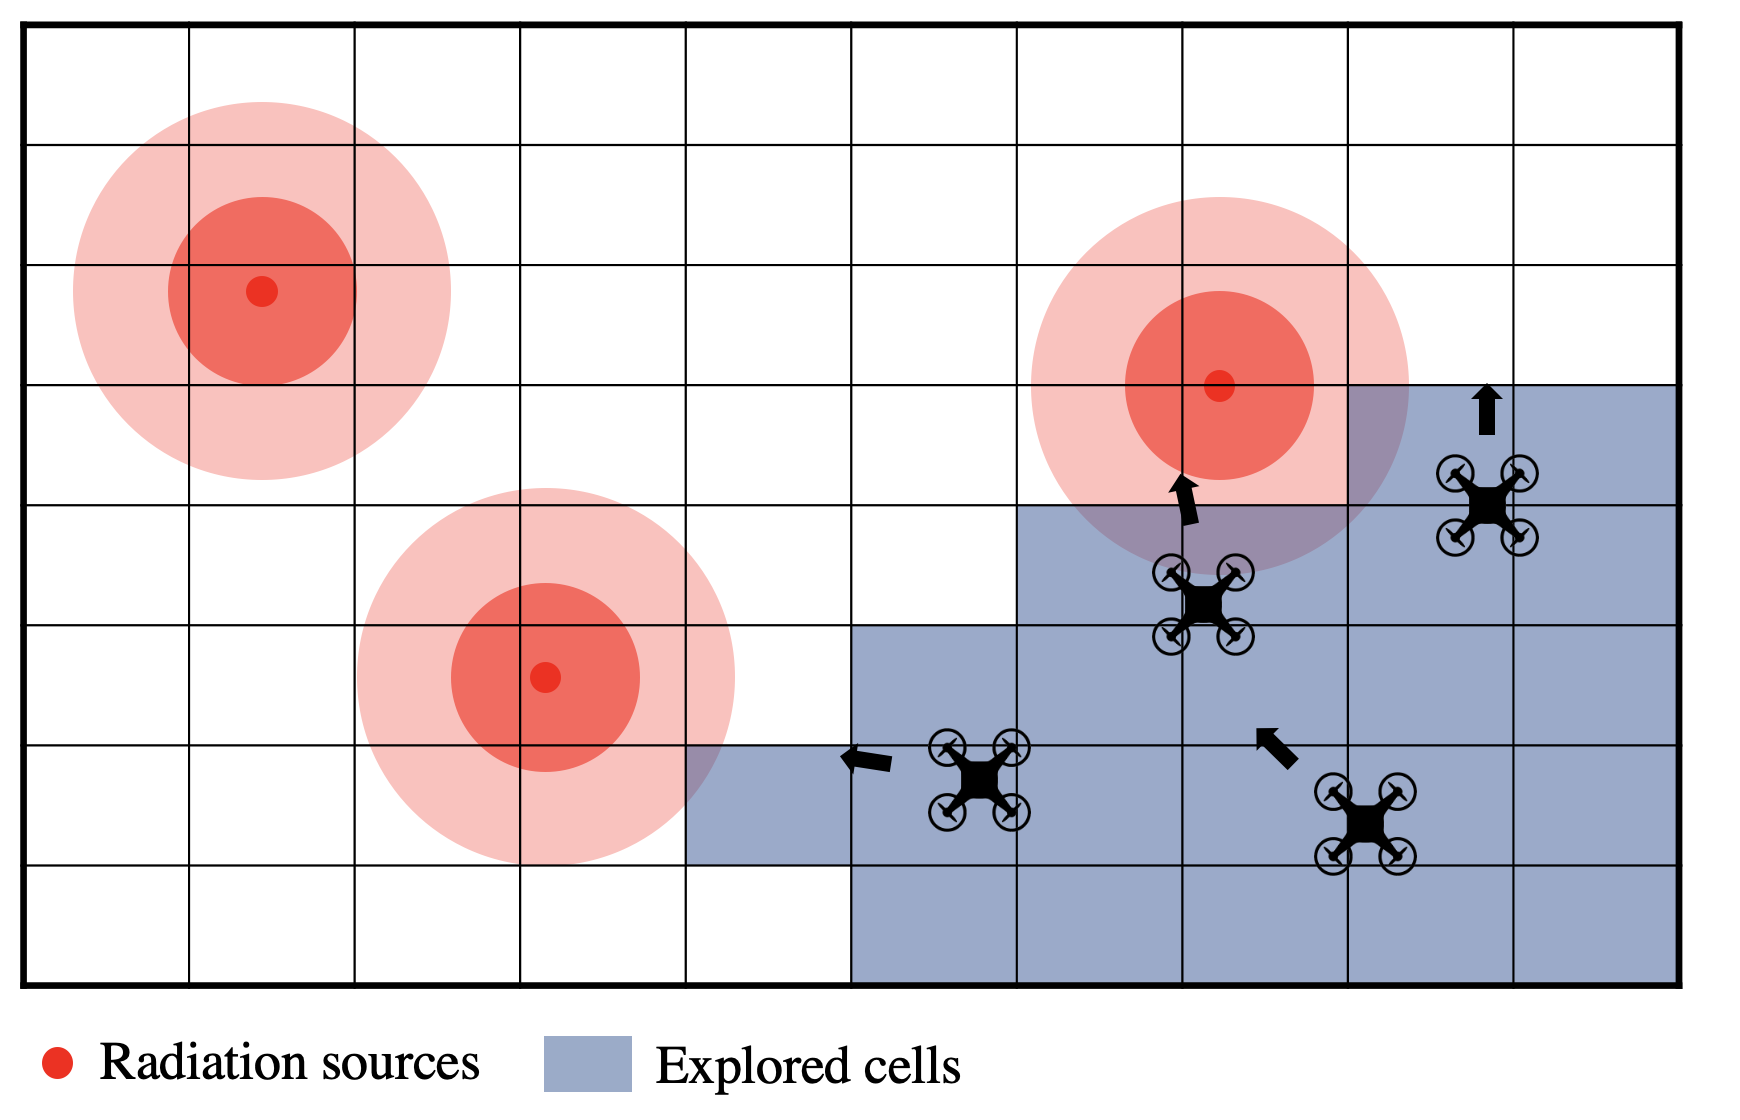
\includegraphics[width=\textwidth]{figures/dora_explorer/risk_aware_b.png}
         \caption{}
         \label{risk_unaware_a}
     \end{subfigure}
     \begin{subfigure}{0.45\textwidth}
         \centering
         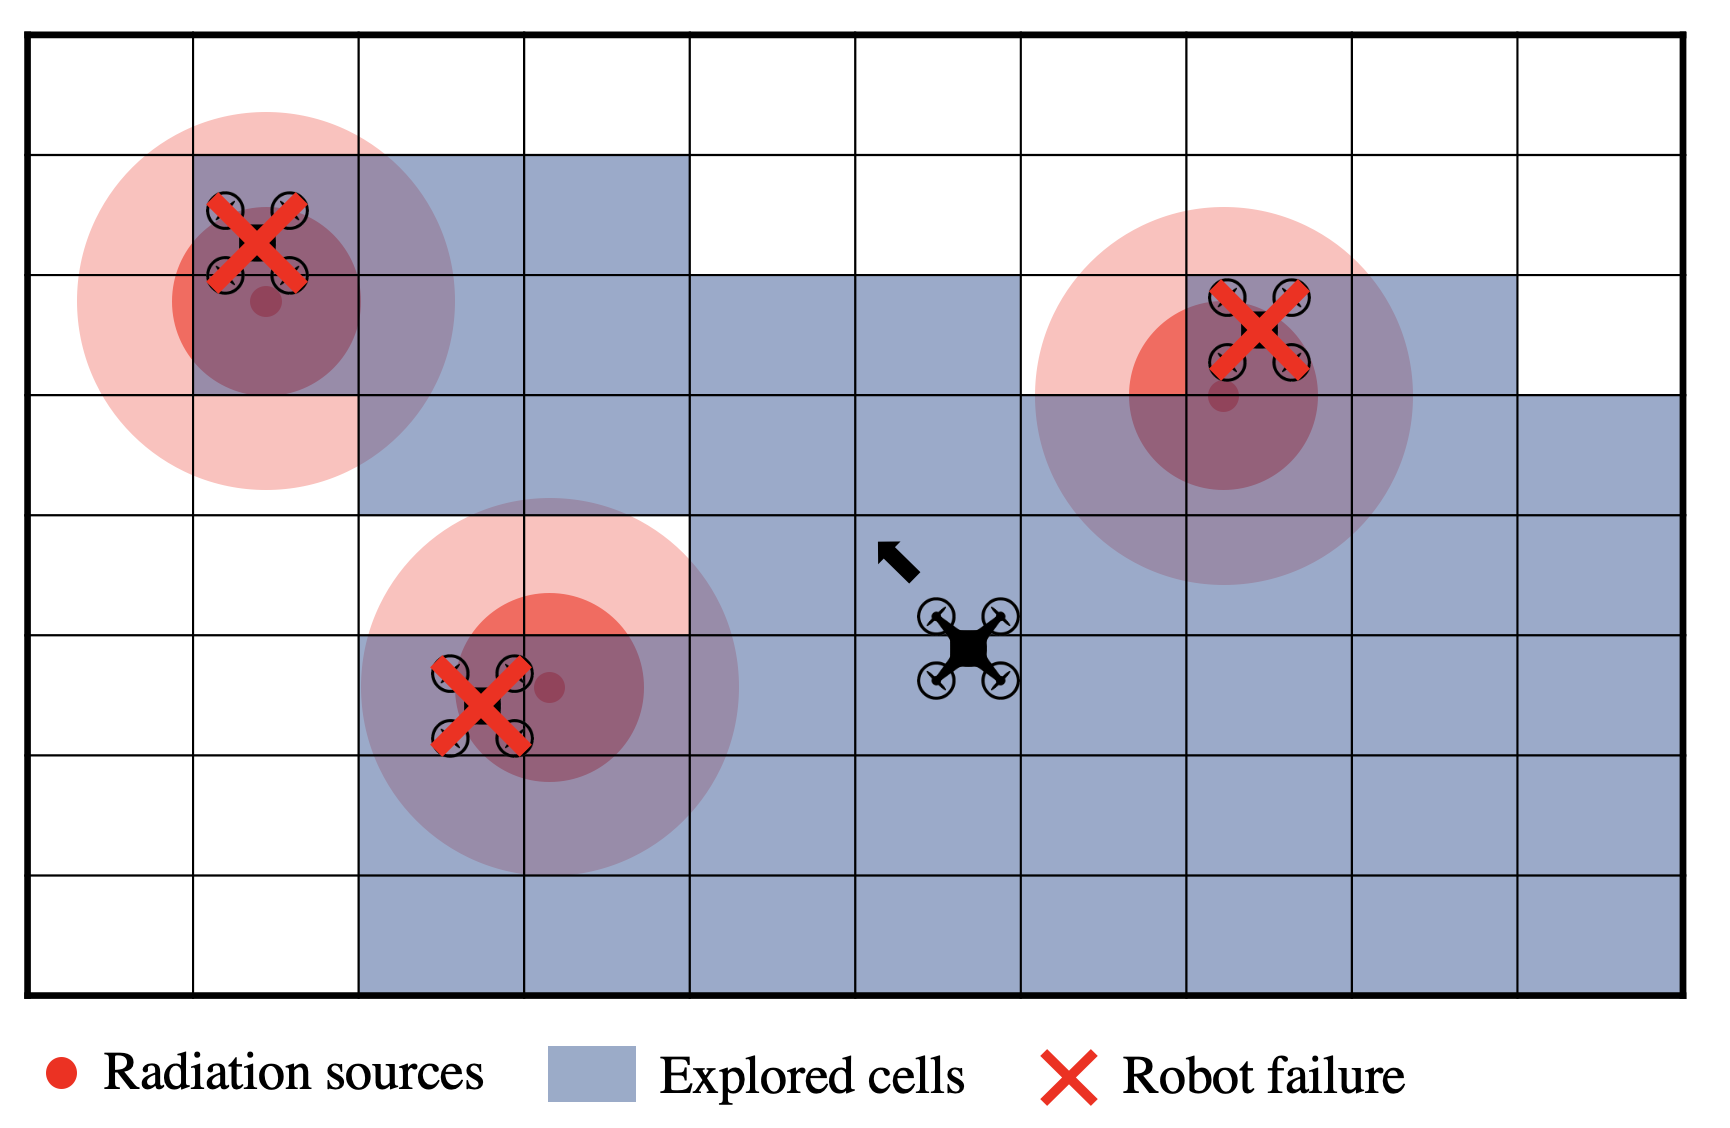
\includegraphics[width=\textwidth]{figures/dora_explorer/risk_unaware_a.png}
         \caption{}
         \label{risk_unaware_b}
     \end{subfigure}
        \caption[Risk-unaware exploration intuition]{Exploration without risk awareness. Fig. \ref{risk_unaware_a}: Robots start exploring but are unable to sense environmental radiation. The only driving force of the algorithm is exploring new cells. Fig. \ref{risk_unaware_b}: Robots fail because they do not discriminate between safe and dangerous cells. Exploration is carried out fewer robots. Exploration efficiency drastically decreases and large areas of the environment remain uncovered.}
        \label{risk_unaware}
\end{figure*}

\begin{figure*}[htbp]
    \centering
    \begin{subfigure}{0.45\textwidth}
         \centering
         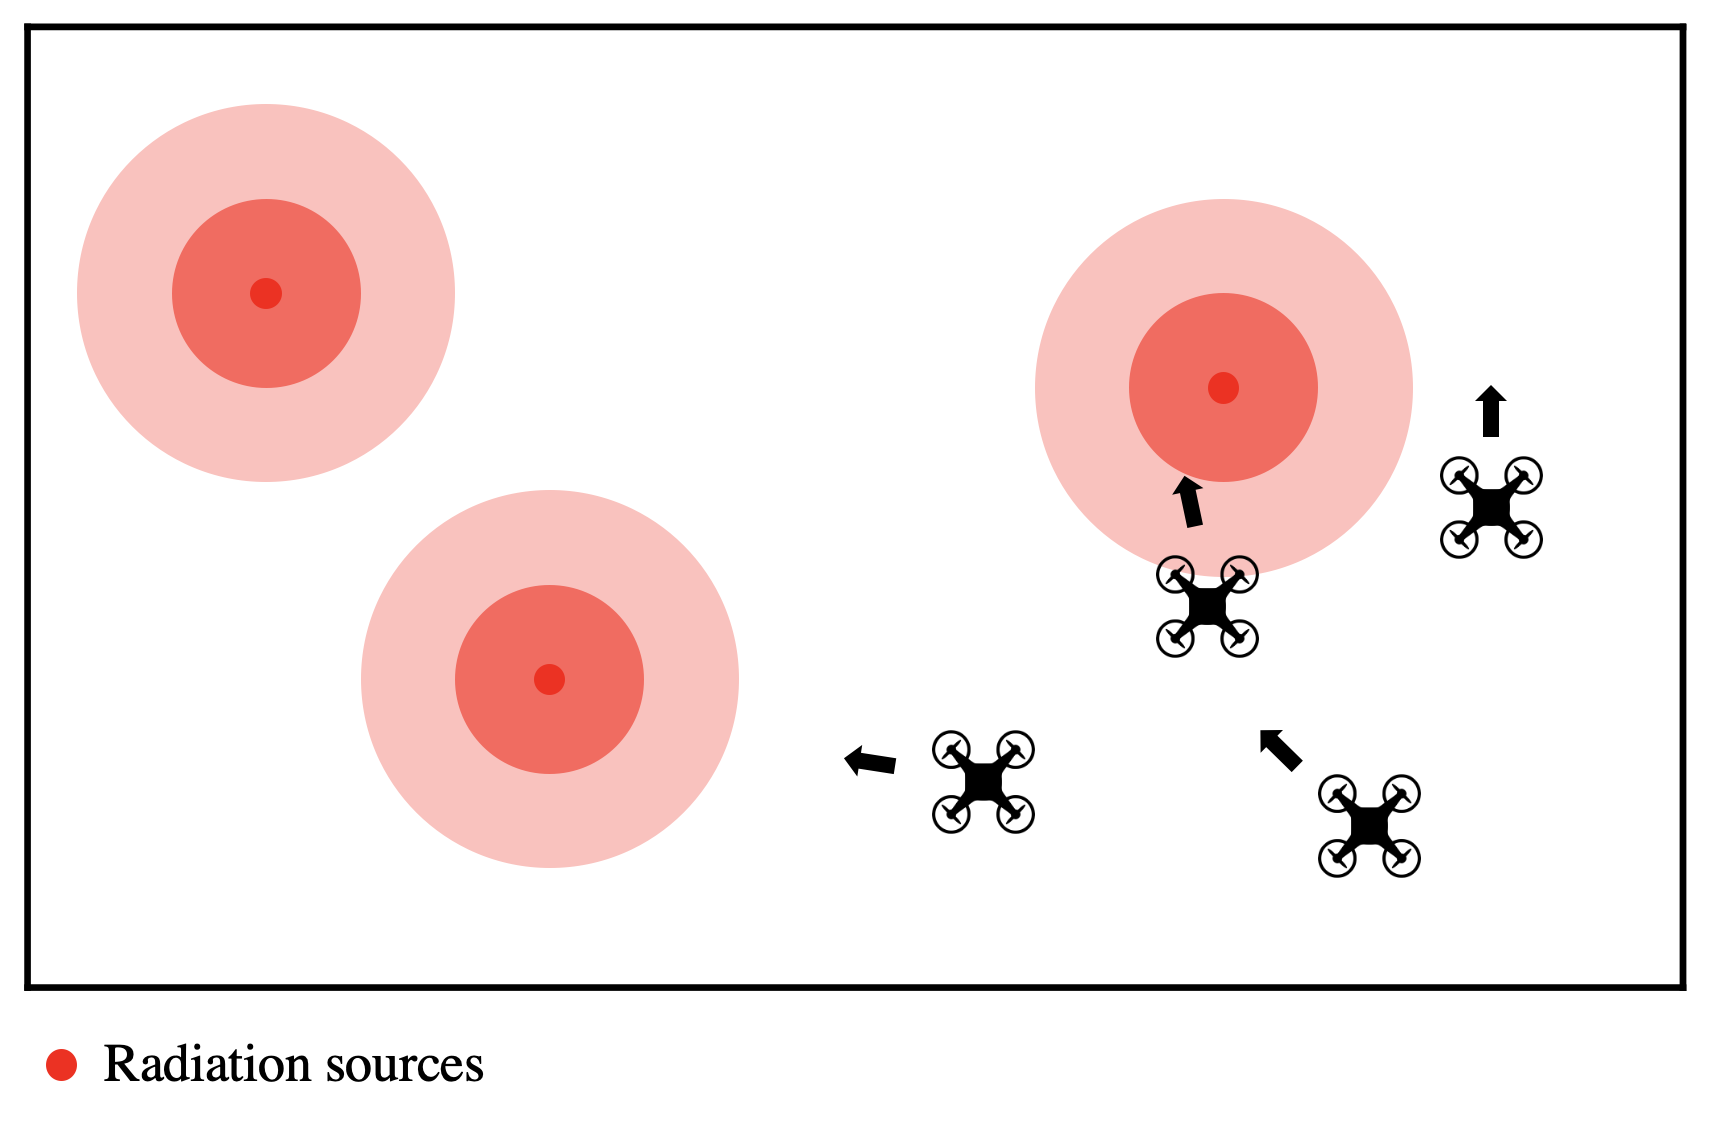
\includegraphics[width=\textwidth]{figures/dora_explorer/risk_aware_a.png}
         \caption{}
         \label{risk_aware_a}
    \end{subfigure}
    \begin{subfigure}{0.45\textwidth}
         \centering
         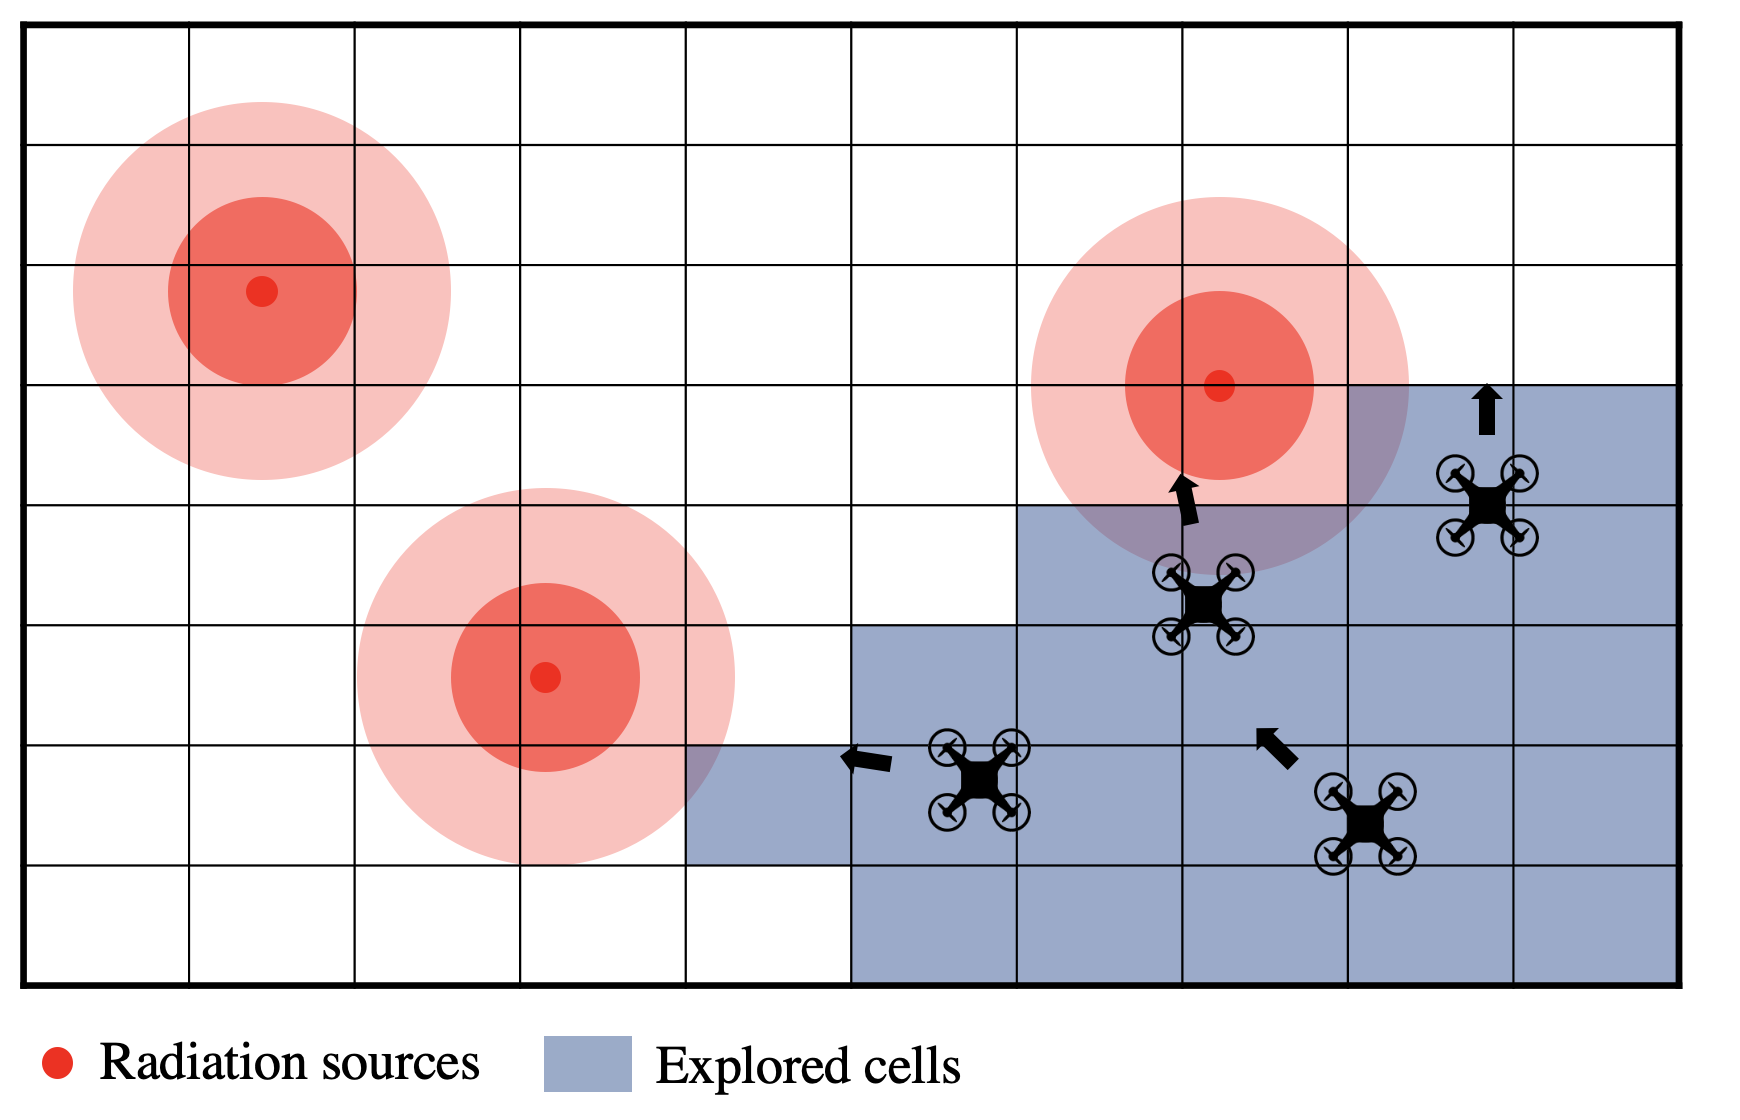
\includegraphics[width=\textwidth]{figures/dora_explorer/risk_aware_b.png}
         \caption{}
         \label{risk_aware_b}
    \end{subfigure}
    \begin{subfigure}{0.45\textwidth}
         \centering
         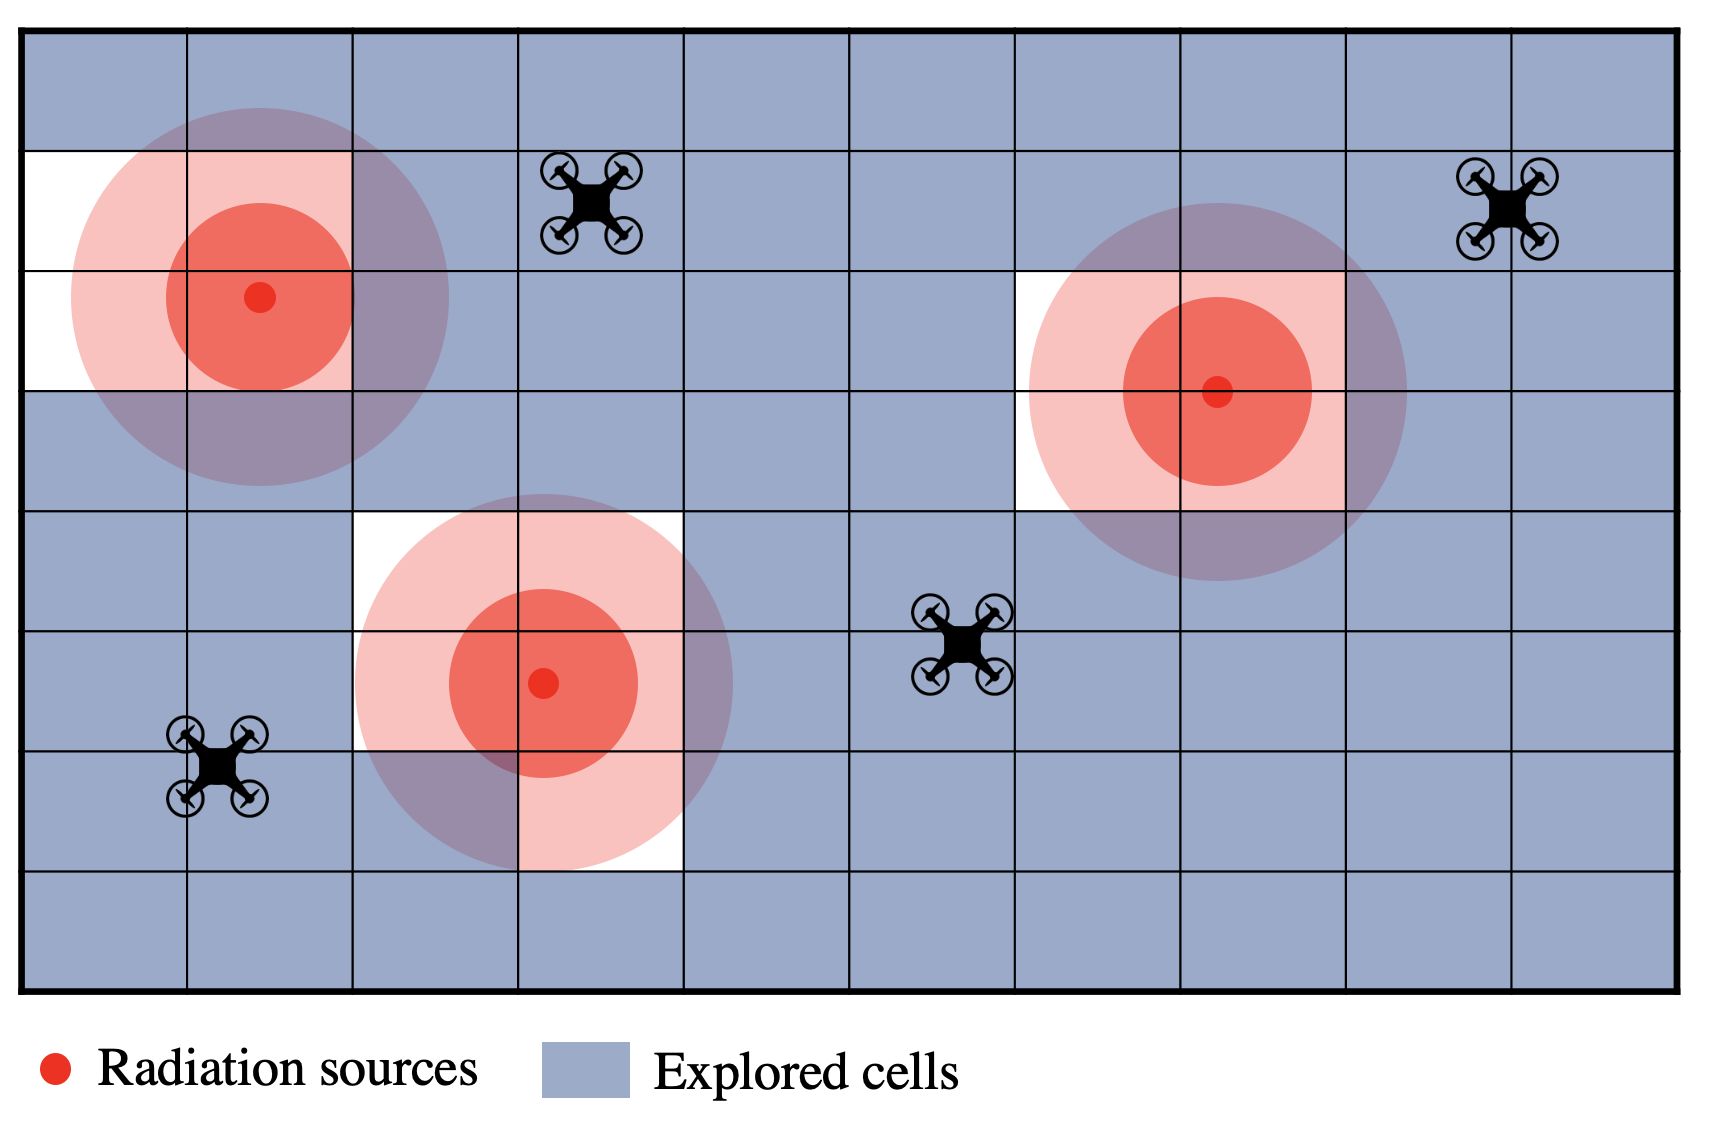
\includegraphics[width=\textwidth]{figures/dora_explorer/risk_aware_c.png}
         \caption{}
         \label{risk_aware_c}
    \end{subfigure}
    \begin{subfigure}{0.45\textwidth}
         \centering
         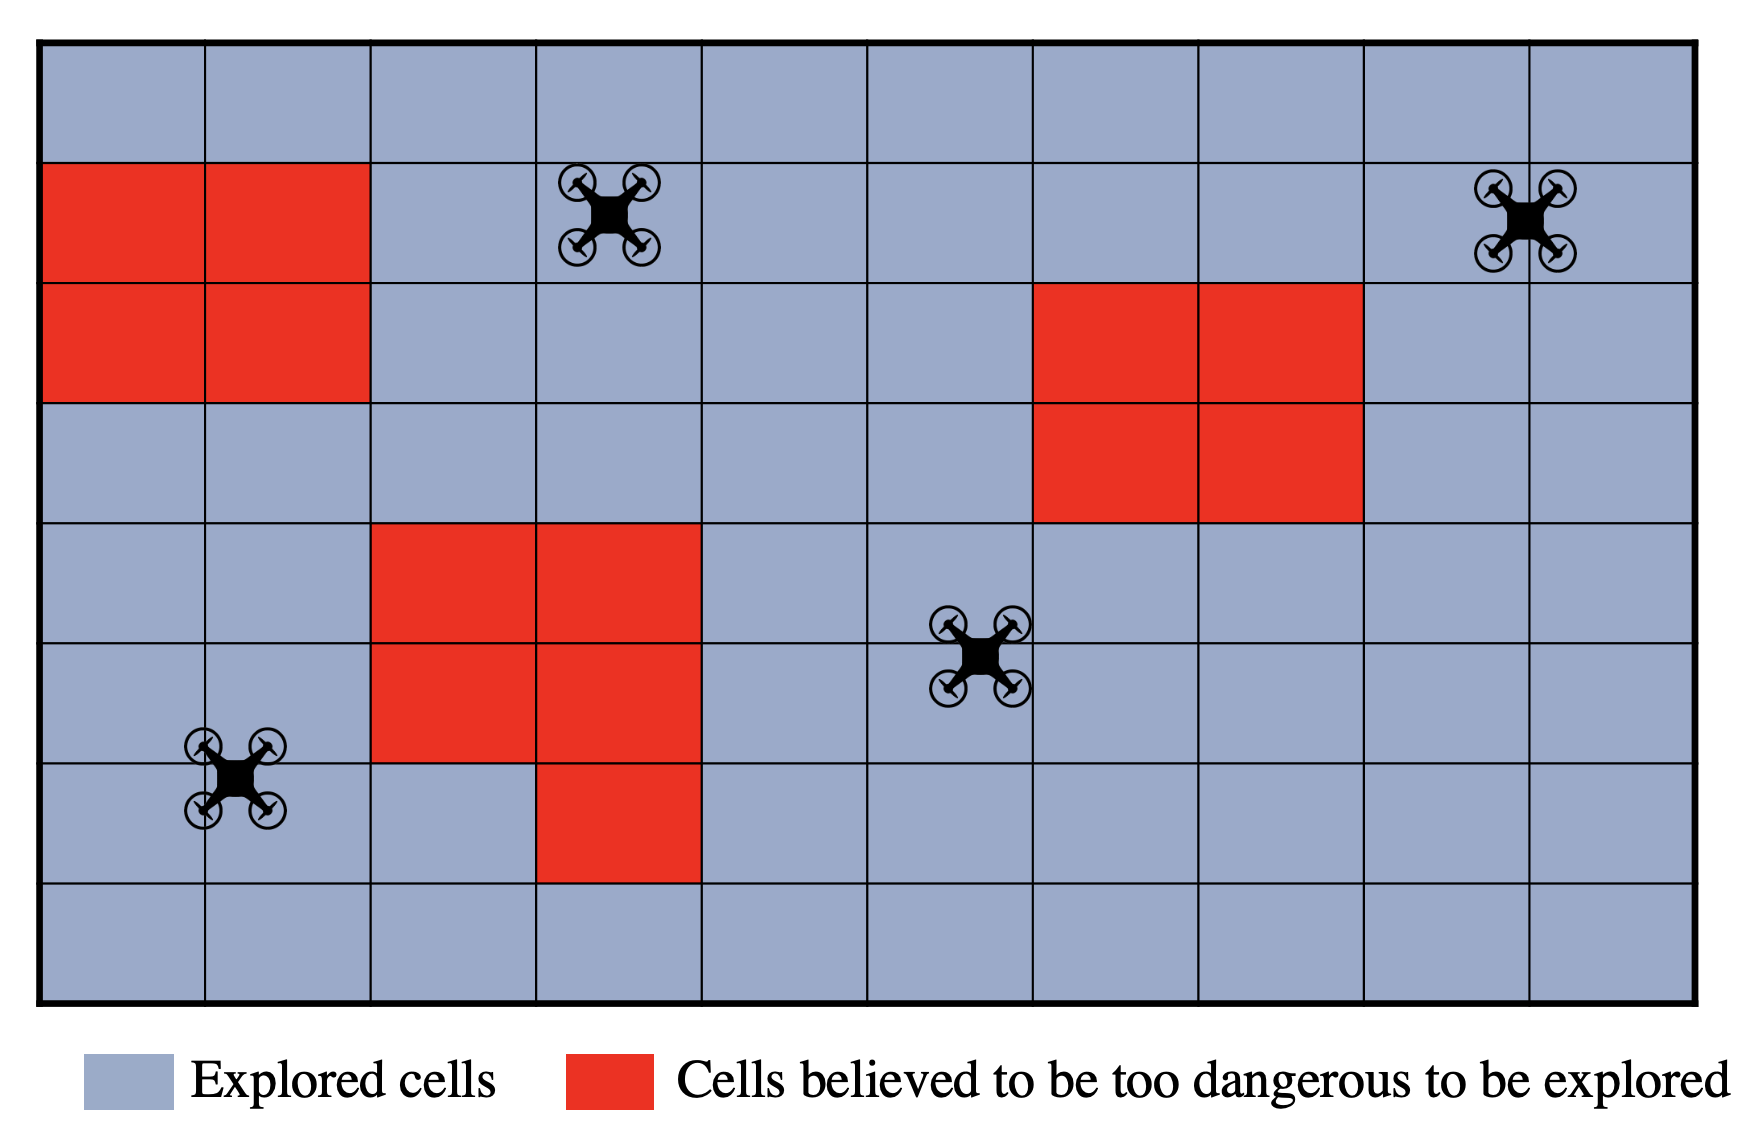
\includegraphics[width=\textwidth]{figures/dora_explorer/risk_aware_d.png}
         \caption{}
         \label{risk_aware_d}
    \end{subfigure}
        \caption[Risk-aware exploration intuition]{Risk aware exploration intuition. Fig. \ref{risk_aware_a}: Robots start exploring hazardous environment. Fig. \ref{risk_aware_b}: A grid is formed. When a new cell from this grid is explored, the sensed radiation is used to update the \ac{DBM}. Fig. \ref{risk_aware_c}: The cells have been mostly covered by the robots. Fig. \ref{risk_aware_d}: Only cells believed to be too dangerous remain unexplored.}
    \label{risk_aware}
\end{figure*}

Finally, to ensure scalability, we made sure \ac{DORA}'s computational and communication costs remained low. They are represented by $C(A, \nu, E)$ and $D(A, \nu, E)$ where $\nu$ is the neighborhood and they are both bounded by $\Theta(|\nu|)$ because of the nature of the algorithm and of the virtual stigmergy.

\section{Experiments}
We performed experiments both in simulations and on physical robots. In both cases, for consistency, we used KheperaIV \cite{kteam2021kheperaiv} robots, which are relatively small and equipped with infrared sensors required for obstacle avoidance. It should be noted that they are capable of wireless networking through the 802.11b/g WiFi protocol, making swarm communication possible. We compared our algorithm with two baselines: \ac{FBE} and a random walk algorithm. The metrics we used to evaluate our system's performance were the number of active (not failed) robots over time, the total number of cells explored over time, and the bandwidth usage. Failures were triggered randomly based on (emulated) perceived radiation from \eqref{eq:radiation_dora}. Detailed motivation for parameter and metric choices can be found in the article.

The first step was to test \ac{DORA} by doing simulations in ARGoS. To verify the effect of swarm size on scalability, we ran our virtual experiments with varying swarm sizes ($N =\{10, 15, 20\}$) deployed randomly in a 20x20m environment with randomly positioned radiation sources and obstacles. To be thorough, we performed 50 simulation runs with 300 time steps each for each algorithm. 

The second step was the physical experiments. We ran them on 5 robots with fewer time steps (200) because of equipment and time constraints respectively. Robot positioning was obtained through motion tracking performed with OptiTrack Motive \cite{optitrack2021motive}. The environment consisted of a 2x2m arena split into a 10x10 cell grid.

\FloatBarrier

\section{Results}
The following shows the average results obtained in the simulation runs as well as those from physical experiment runs.

Fig. \ref{results:dora_explored} shows that \ac{DORA} attains similar terrain coverage to \ac{FBE}. Moreover, the performance gap between the two reduces as $N$ increases, showing good scalability from \ac{DORA}. Both algorithms outperform the random walk one by far. Interestingly, \ac{DORA} covered more cells than \ac{FBE} in physical experiments. This is probably because the small size of the arena presented a pathological case for \ac{FBE}. 

\begin{figure*}
    \centering
    \begin{subfigure}{0.45\textwidth}
        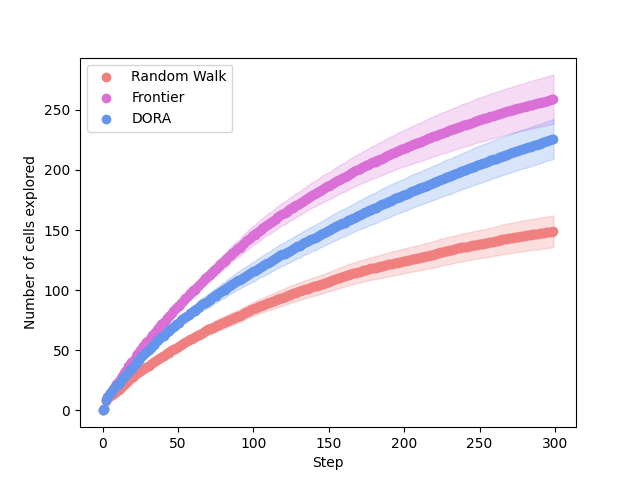
\includegraphics[width=\textwidth]{figures/dora_explorer/explored_10.png}
        \caption{N=10 robots}
        \label{results:explored10}
    \end{subfigure}
    \begin{subfigure}{0.45\textwidth}
        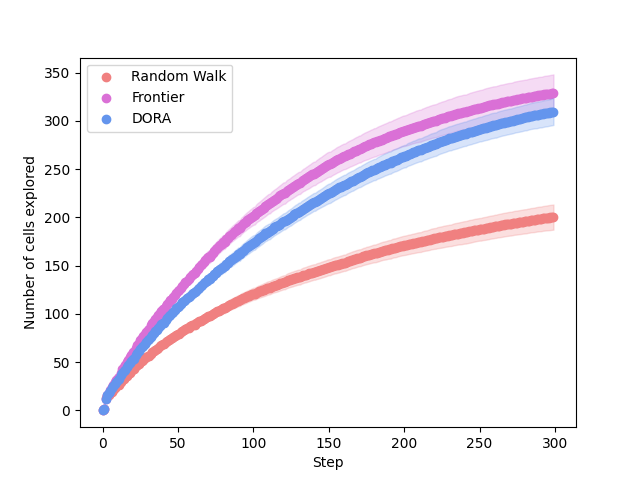
\includegraphics[width=\textwidth]{figures/dora_explorer/explored_15.png}
        \caption{N=15 robots}
        \label{results:explored15}
    \end{subfigure}
    \begin{subfigure}{0.45\textwidth}
        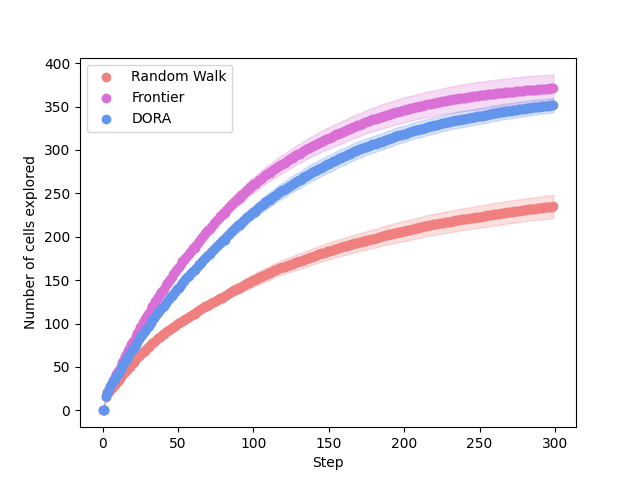
\includegraphics[width=\textwidth]{figures/dora_explorer/explored_20.png}
        \caption{N=20 robots}
        \label{results:explored20}
    \end{subfigure}
    \begin{subfigure}{0.45\textwidth}
        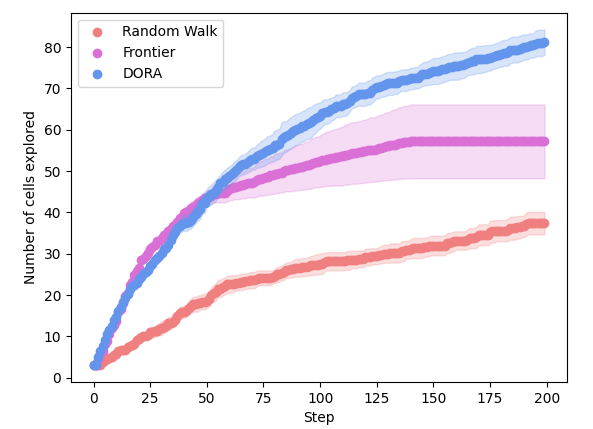
\includegraphics[width=\textwidth]{figures/dora_explorer/explored_real.png}
        \caption{N=5 physical robots}
        \label{results:cells_explored_physical}
    \end{subfigure}
    \caption[DORA cell exploration performance]{Performance comparison of \ac{DORA}, \ac{FBE} and random walk for number of explored cells over time.  Fig. \ref{results:explored10}, \ref{results:explored15}, \ref{results:explored20} are for simulations; Fig. \ref{results:cells_explored_physical} is for physical experiments.}
    \label{results:dora_explored}
\end{figure*}

Where \ac{DORA} truly shows its worth is in Fig. \ref{results:dora_active}, in which the number of active robots over time is presented. Indeed, in every experiment scenario, \ac{DORA} experienced far fewer robot failures than both benchmark algorithms. As for terrain coverage, \ac{DORA}'s performance improves with respect to the other algorithms as the number of robots involved increases. This further shows our algorithm's scalability.

\begin{figure*}
    \centering
    \begin{subfigure}{0.45\textwidth}
        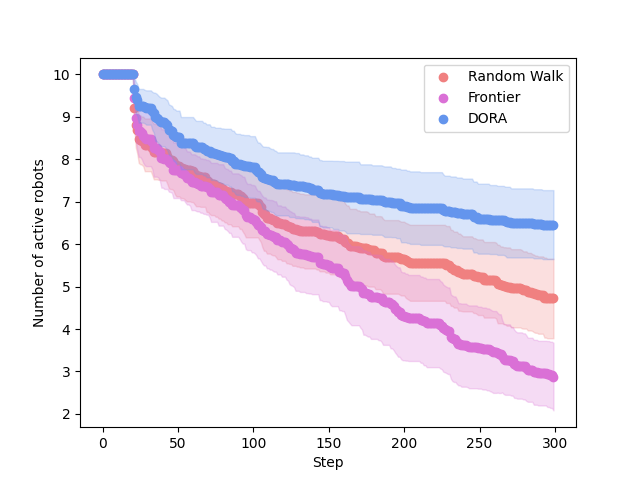
\includegraphics[width=\textwidth]{figures/dora_explorer/activerobots_10.png}
        \caption{N=10 robots}
        \label{results:failures10}
    \end{subfigure}
    \begin{subfigure}{0.45\textwidth}
        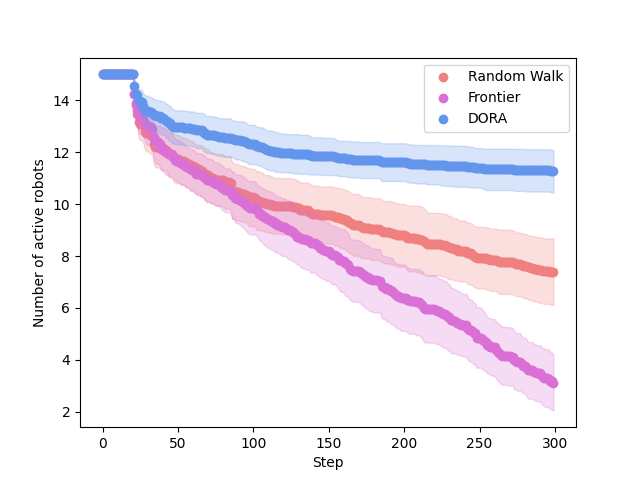
\includegraphics[width=\textwidth]{figures/dora_explorer/activerobots_15.png}
        \caption{N=15 robots}
        \label{results:failures15}
    \end{subfigure}
    \begin{subfigure}{0.45\textwidth}
        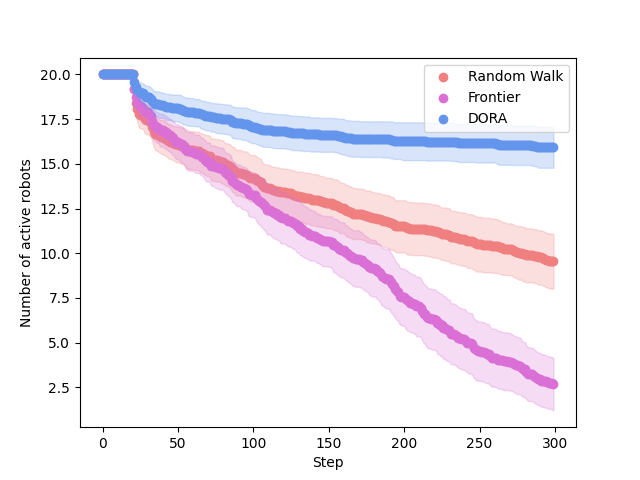
\includegraphics[width=\textwidth]{figures/dora_explorer/activerobots_20.png}
        \caption{N=20 robots}
        \label{results:failures20}
    \end{subfigure}
    \begin{subfigure}{0.45\textwidth}
        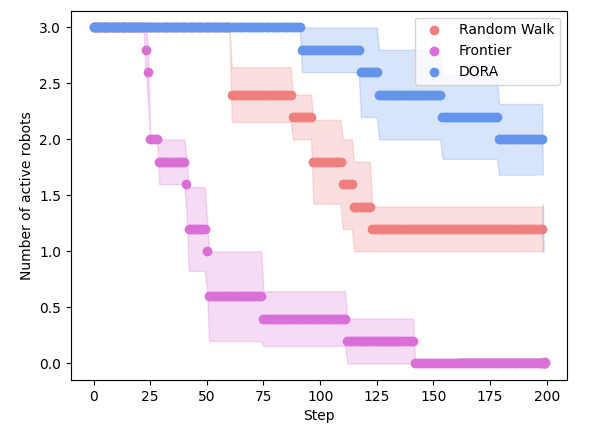
\includegraphics[width=\textwidth]{figures/dora_explorer/activerobots_real.png}
        \caption{N=5 physical robots}
        \label{results:active_robots_physical}
    \end{subfigure}
    \caption[DORA survival performance]{Performance comparison of \ac{DORA}, \ac{FBE} and random walk for number of active robots over time. Fig. \ref{results:failures10}, \ref{results:failures15}, \ref{results:failures20} are for simulations; Fig. \ref{results:active_robots_physical} is for physical experiments.} 
    \label{results:dora_active}
\end{figure*}

Intuition for how \ac{DORA} results from Fig.\ref{results:dora_explored} and Fig. \ref{results:dora_active} are related can be gained by observing Fig. \ref{results:belief}. Whereas \ac{FBE} visited the areas around the radiation sources (as can be seen by the cells with a high radiation level), \ac{DORA} avoided them. This results in a slightly lower exploration coverage, but in a much lower failure rate.

\begin{figure*}
    \centering
    % \begin{subfigure}{0.45\textwidth}
    %     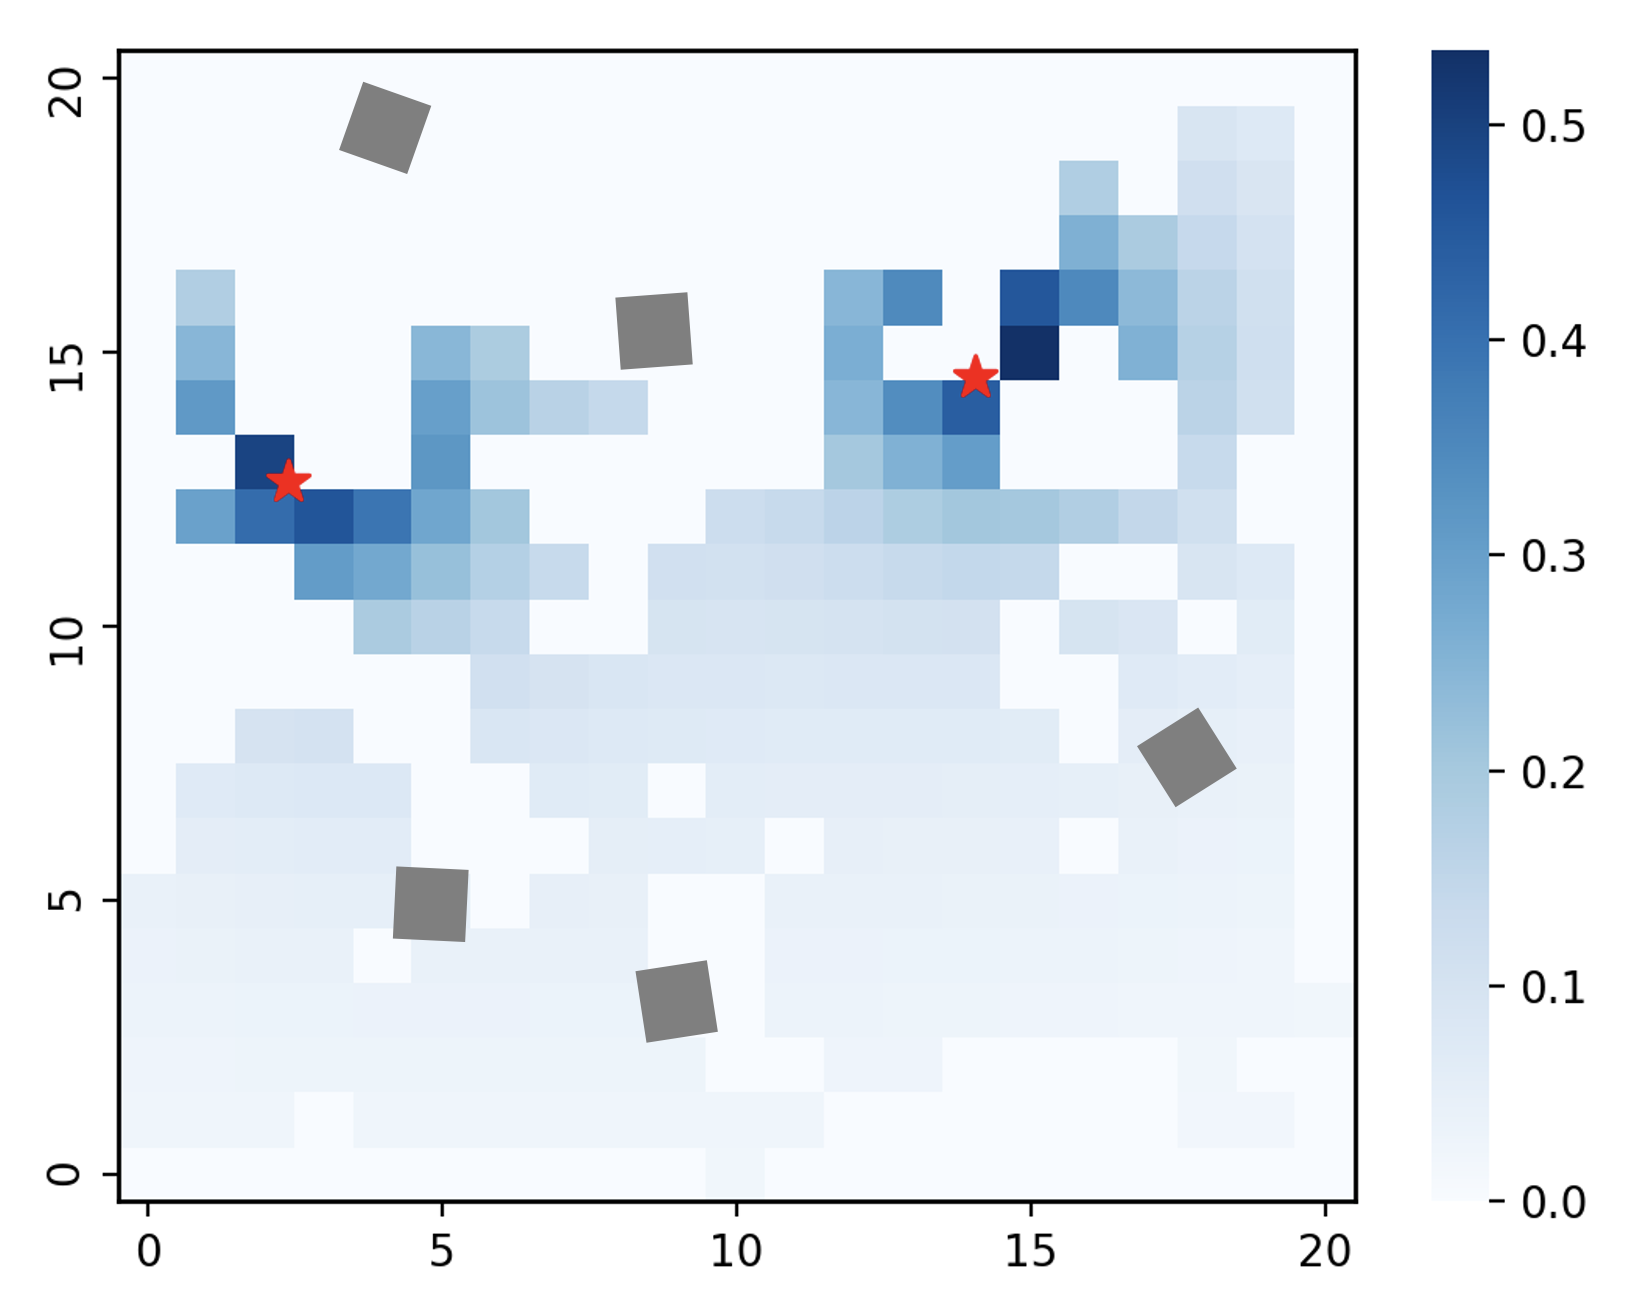
\includegraphics[width=\textwidth]{figures/dora_explorer/heatmap_random.png}
    %     \caption{Random walk}
    %     \label{results:beliefrandom}
    % \end{subfigure}
    \begin{subfigure}{0.45\textwidth}
        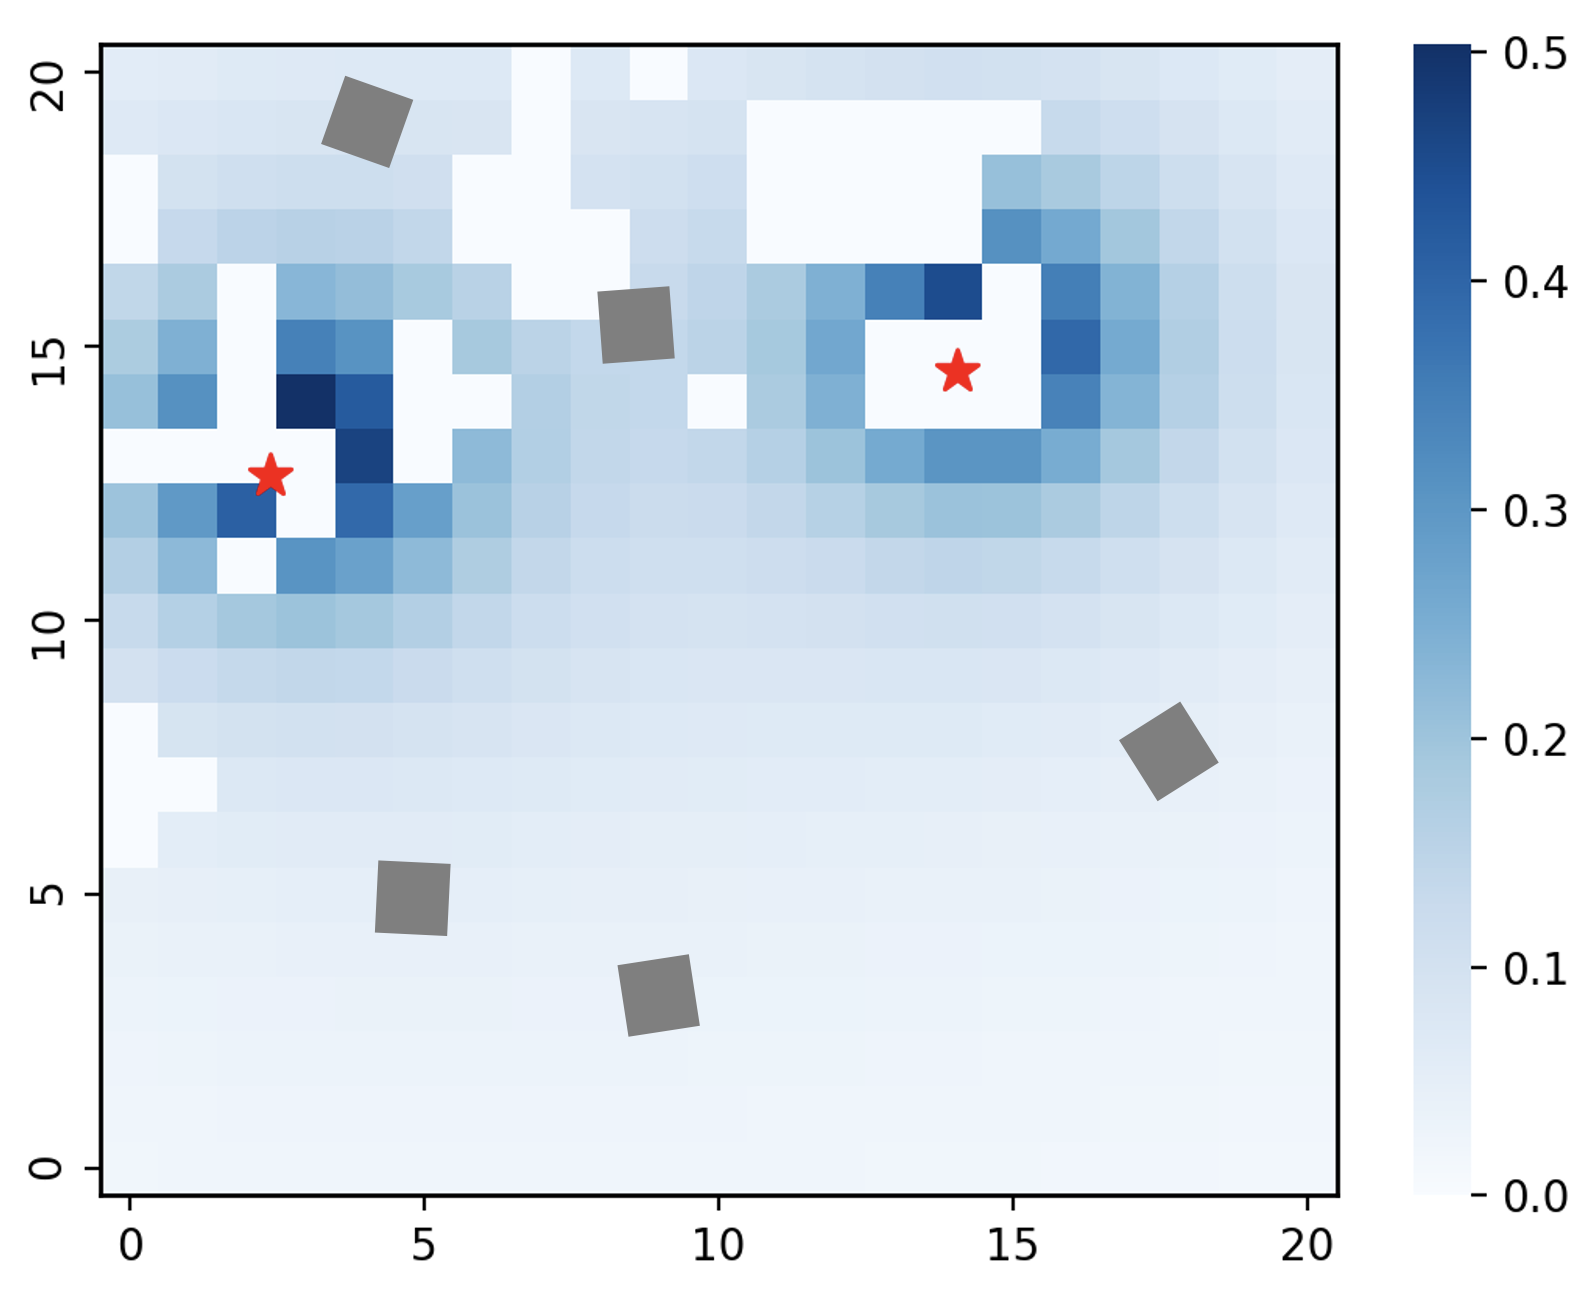
\includegraphics[width=\textwidth]{figures/dora_explorer/heatmap_frontier.png}
        \caption{\ac{FBE}}
        \label{results:belieffrontier}
    \end{subfigure}
    \begin{subfigure}{0.45\textwidth}
        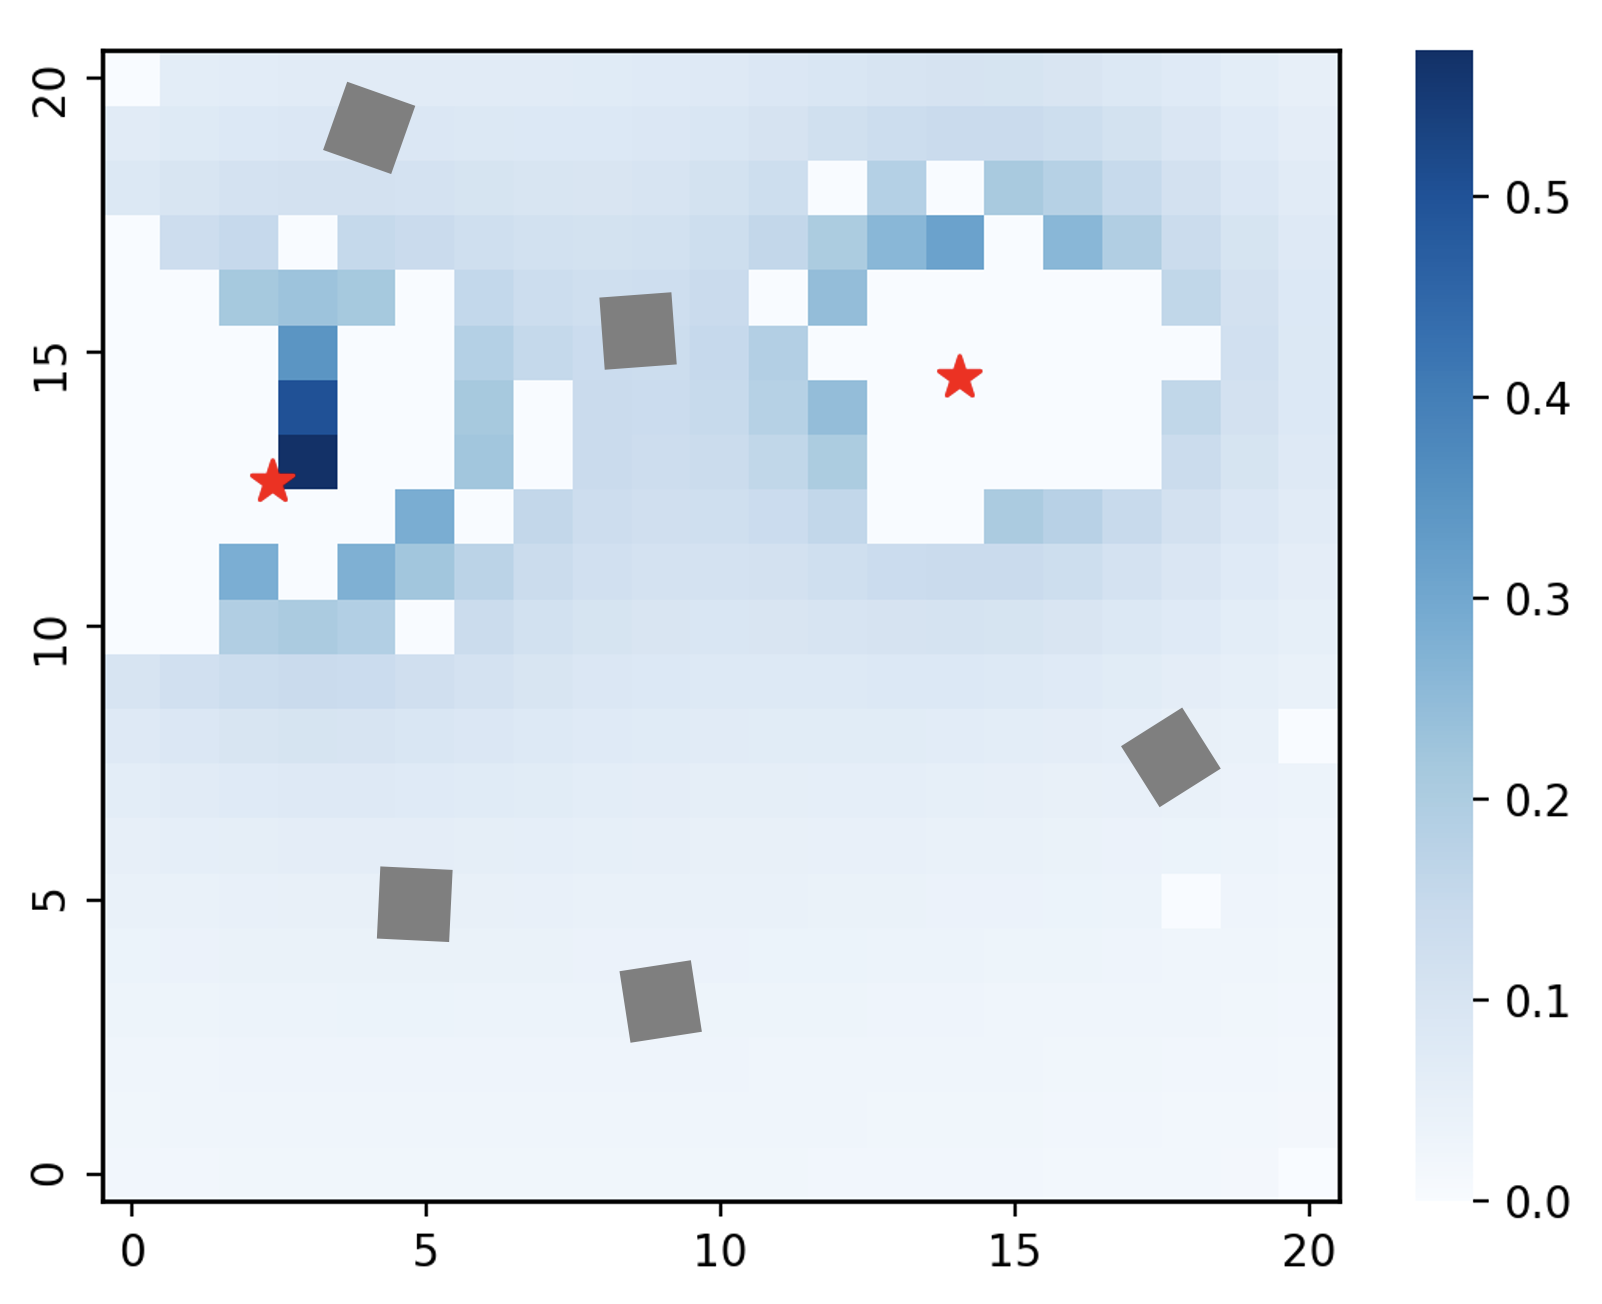
\includegraphics[width=\textwidth]{figures/dora_explorer/heatmap_dora.png}
        \caption{\ac{DORA}}
        \label{results:beliefdora}
    \end{subfigure}
    \caption[DORA radiation belief maps]{Radiation belief maps of the 20x20m environment for each exploration algorithm of one specific simulation. Blank cells are unvisited areas, red stars are the point radiation sources and grey squares are the randomly generated obstacles.}
    \label{results:belief}
\end{figure*}

In Fig. \ref{results:communicationCosts}, we can see the amount of data exchanged by robots in the simulations conducted with \ac{DORA} and \ac{FBE}. The takeaway is that \ac{DORA} outperforms \ac{FBE} by a significant margin for this metric, and that communication costs are aligned with the theoretical values from \ref{dora_system_model}. This metric was not calculated for the random walk algorithm as it does not require any coordination nor communication. It was not measured in physical experiments.

\begin{figure}[htbp]
    \centering
    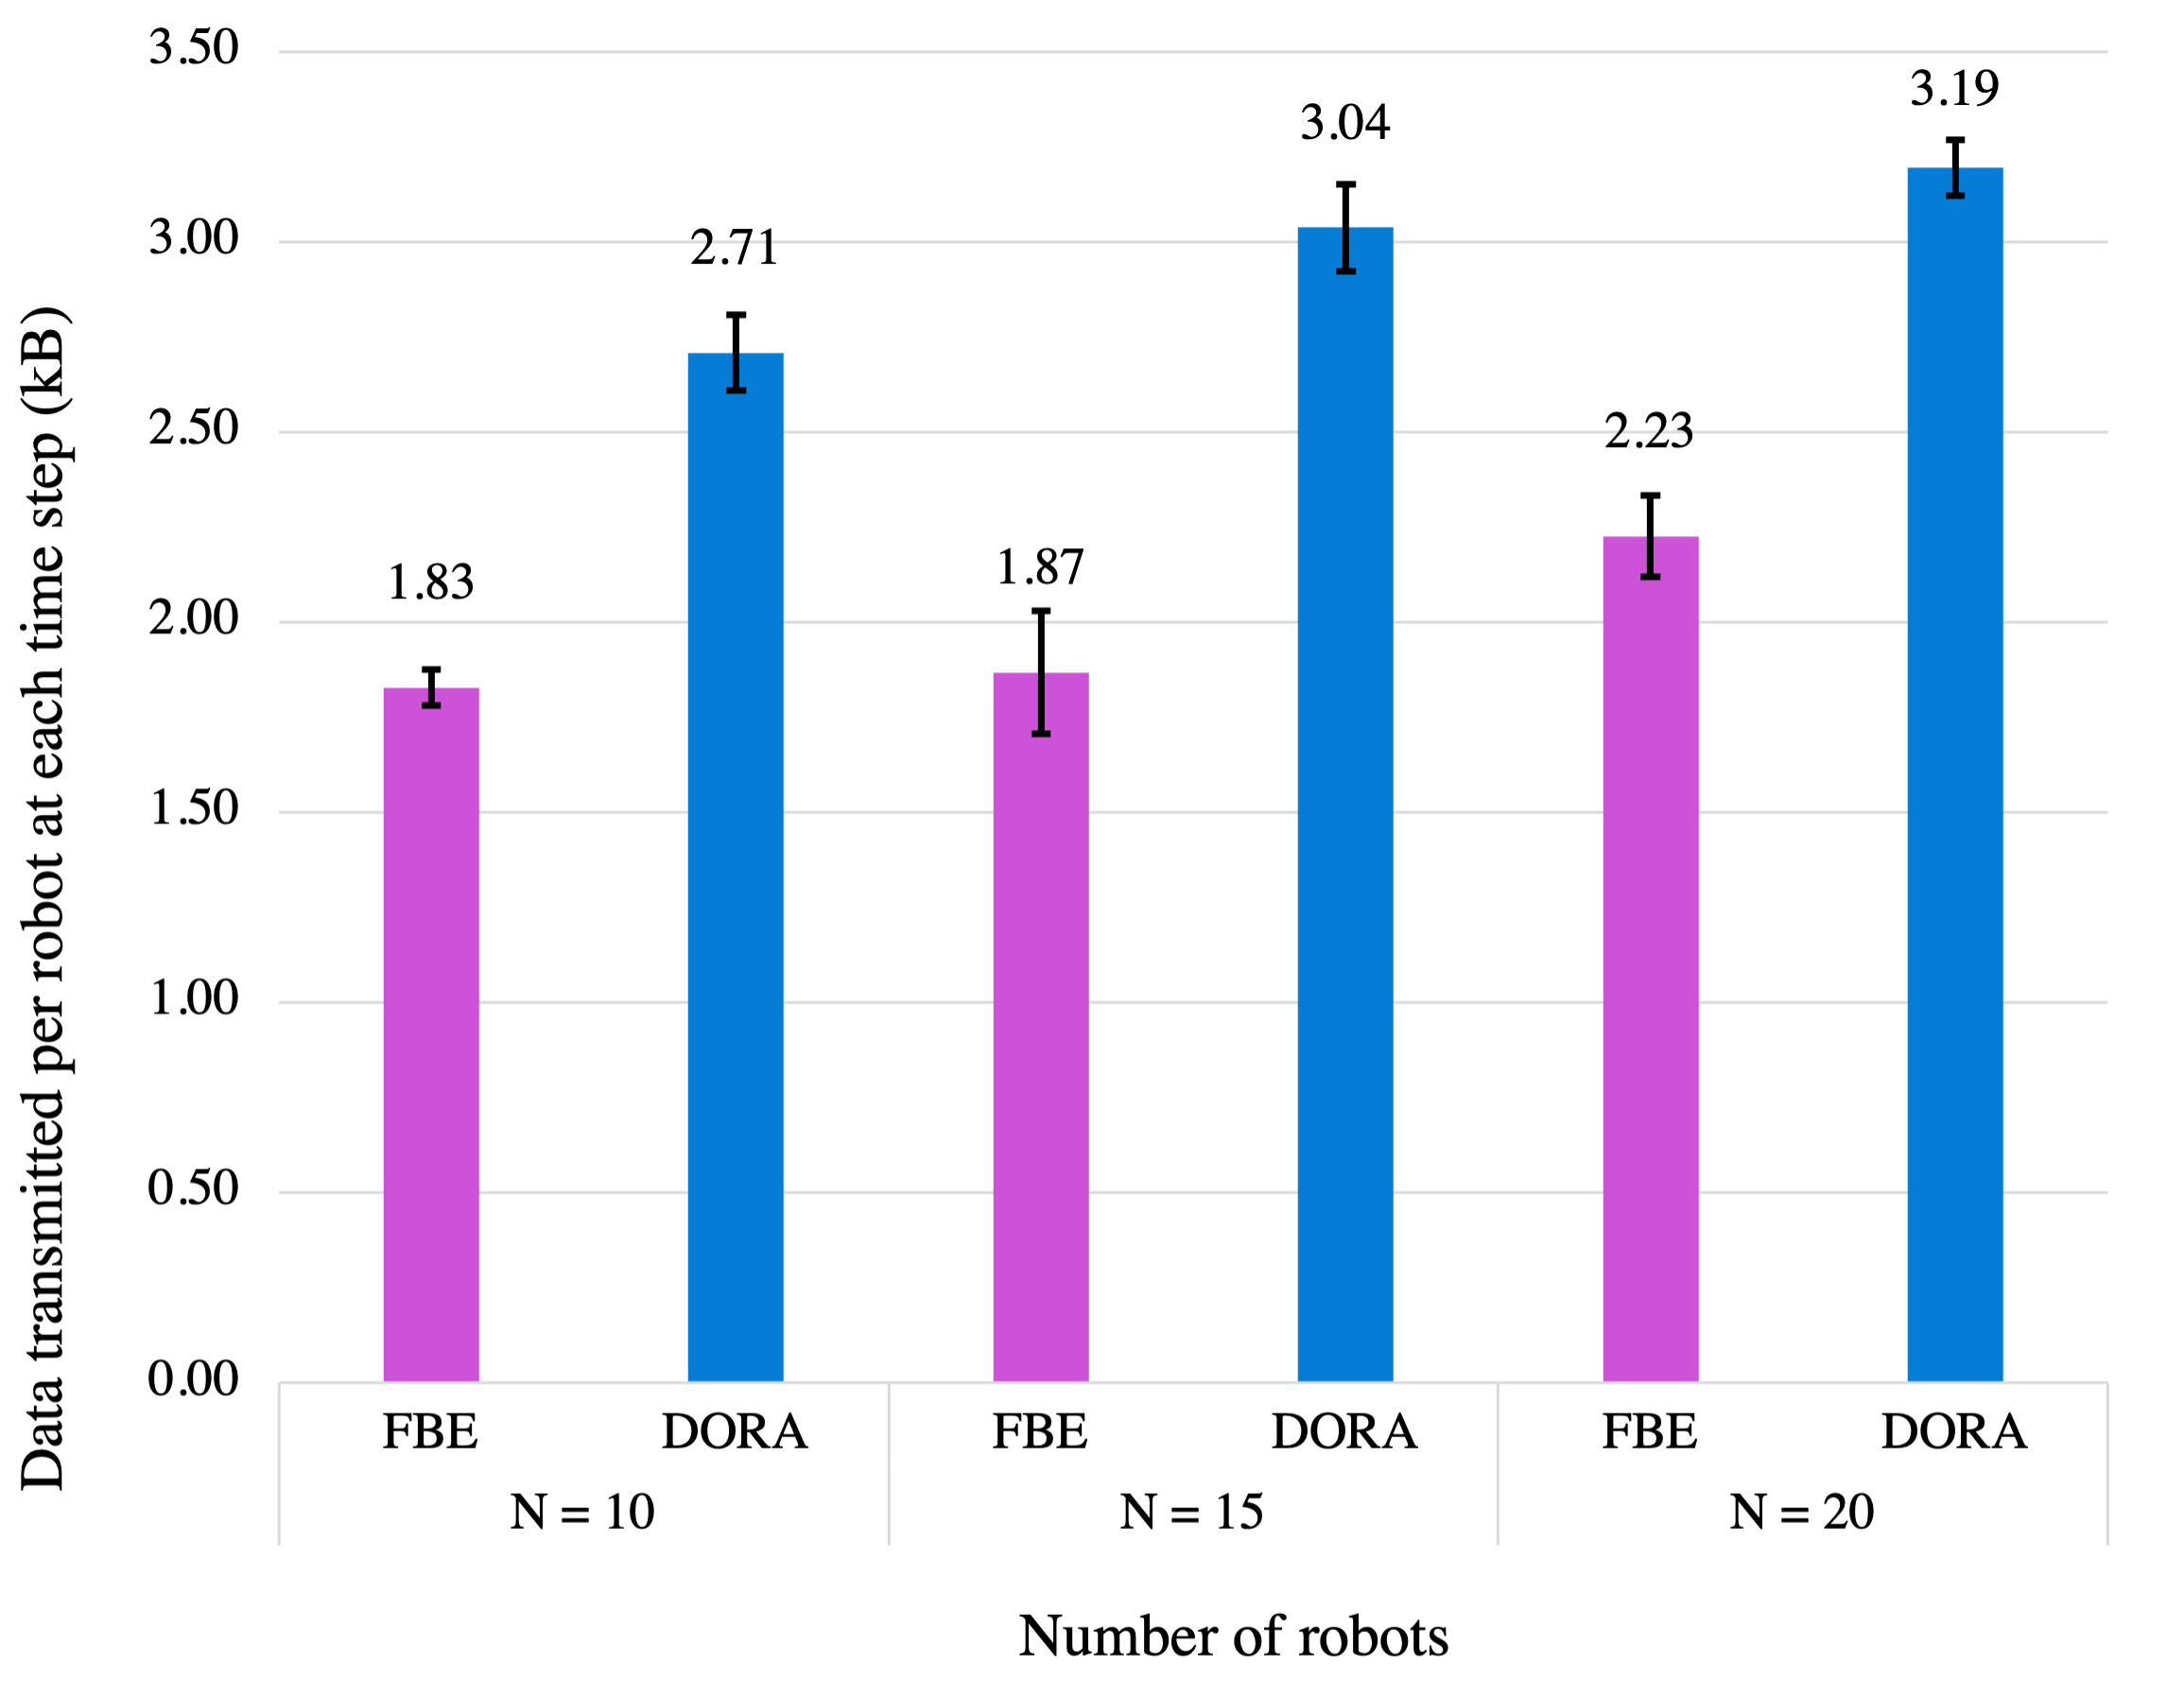
\includegraphics[width=0.95\textwidth]{figures/dora_explorer/communication.png}
    \caption[DORA communication costs]{Communication costs for \ac{DORA} and \ac{FBE}}
    \label{results:communicationCosts}
\end{figure}

\FloatBarrier

\section{Conclusion}
We presented \ac{DORA} Explorer, a novel lightweight risk-aware exploration
algorithm that minimizes the risk to which robots expose themselves in
order to maximize the amount of ground they will be able to cover
without failing. We expected that our exploration algorithm, which
leverages \ac{DBM}s, would greatly outperform non-coordinated solutions,
and this has been the case. Indeed, it succeeded in reducing
considerably the likeliness of robot failures while keeping similar
ground coverage performance compared to other solutions proposed in
the literature. \ac{DORA} also showed good scalability thanks to its low
communication costs. It also showed applicability to real world
scenarios through experiments with physical robots.

In future work, it could be interesting to allow \ac{DORA} to become more
or less risk-avoiding depending on the changing needs of the
situation. For example, in a search-and-rescue scenario, an increasing
urgency to rescue victims could motivate the willingness to take more
risks as time progresses. Also, more experiments could be conducted by
testing \ac{DORA} Explorer on a larger team of physical robots exploring
larger outdoor environments. Further applications of \ac{DORA} could
include using the generated risk belief map to determine robots'
fitness to store data in distributed storage systems like SwarmMesh
\cite{majcherczykSwarmmesh2020}, with robots assigned to tasks in
dangerous regions being discouraged from storing sensitive
information. Additionally, in this work we considered that the risk
associated with the environment can be sensed by the robots. However,
in some scenarios, the risk cannot be directly perceived by any
sensors. In these cases, the belief map could be constructed using the
previous failures of the agents by assigning risk to areas where
failures have been detected in the past.
             % Second thème (Doctorat) ou "Résultats théoriques et expérimentaux" (Maîtrise).
\Chapter{CONCLUSION}\label{sec:Conclusion}
The objective of the research conducted for this thesis was to design risk-aware algorithms to improve the resiliency of swarm robotics systems. RASS and DORA are both meant to be used as part of other other systems, and thus to be stepping stones towards trustworthy industrial applications.

%%
%%  SYNTHESE DES TRAVAUX / SUMMARY OF WORKS
%%
\section{Summary of Works}
Texte / Text.

%%
%%  LIMITATIONS
%%
\section{Limitations}\label{sec:Limitations}
Robot-simulation gap would require further experiments.

Physical scalability, in both RASS and DORA, has not been extensively tested. This is due to a limited number of robots available for each experiment. In RASS's case, we could only use 5 CogniFlies \cite{de2021flexible}, and for DORA, we only had access to 5 KheperaIV robots.

%%
%%  AMELIORATIONS FUTURES *-/ FUTURE RESEARCH
%%
\section{Future Research}
Adapting solutions to heterogeneous swarms with different resistance to risk could prove an interesting challenge and would show the adaptability of both RASS and DORA to more diverse scenarios in which swarms can retain their group performance advantage derived from heterogeneity \cite{ferrante2015evolution}. Testing in more challenging environments (rugged terrain, terrains with hidden lines of sights, dynamic risk conditions, etc.). Further improvements could be integrated to the system, such as improvements to security by using techniques like sinkhole detection proposed by \cite{abdullah2015detecting}.         % Conclusion.
%\backmatter
\ifthenelse{\equal{\Langue}{english}}{
	\renewcommand\bibname{REFERENCES}
	\bibliography{Document}
	\bibliographystyle{IEEEtran}			% Bibliography style. 
}{
	\renewcommand\bibname{RÉFÉRENCES}
	\bibliography{Document}
	\bibliographystyle{IEEEtran-francais}    % Style de la bibliographie. 
}

%%% ANNEXES
% \ifthenelse{\equal{\AnnexesPresentes}{O}}{
% 	\appendix%
% 	\newcommand{\Annexe}[1]{\annexe{#1}\setcounter{figure}{0}\setcounter{table}{0}\setcounter{footnote}{0}}%
% 	%%
%%  Annexes
%%
%%  Note: Ne pas modifier la ligne ci-dessous. / Do not modify the following line.
\ifthenelse{\equal{\Langue}{english}}{
	\addcontentsline{toc}{compteur}{APPENDICES}
}{
	\addcontentsline{toc}{compteur}{ANNEXES}
}
%%
%%
%%  Toutes les annexes doivent être inclues dans ce document
%%  les unes à la suite des autres.
%%  All annexes must be included in this document one after the other.
\Annexe{Démo}
Texte de l'annexe A\@. Remarquez que la phrase précédente se termine
par une lettre majuscule suivie d'un point. On indique explicitement
cette situation à \LaTeX{} afin que ce dernier ajuste correctement
l'espacement entre le point final de la phrase et le début de la
phrase suivante.


\begin{landscape}
\Annexe{Encore une annexe / Another Appendix}
Texte de l'annexe B\@ en mode «landscape».
\end{landscape}

\Annexe{Une dernière annexe / The Last Appendix}
Texte de l'annexe C\@.
}
% {}
\end{document}
